% arara: xelatex
%% arara: biber
% arara: xelatex



\documentclass[12pt]{article} % размер шрифта


\usepackage{tikz} % картинки в tikz
\usepackage{microtype} % свешивание пунктуации

\usepackage{comment} % для комментариев

\usepackage{array} % для столбцов фиксированной ширины

\usepackage{url} % для вставки ссылок \url{...}

\usepackage{indentfirst} % отступ в первом параграфе

\usepackage{sectsty} % для центрирования названий частей
\allsectionsfont{\centering} % приказываем центрировать все sections

\usepackage{amsthm} % теоремы и доказательства

\theoremstyle{definition} % прямой шрифт в условии теорем
\newtheorem{theorem}{Теорема}[section]


\usepackage[colorlinks, hyperindex, unicode, breaklinks]{hyperref} % гиперссылки в pdf


\usepackage{amsmath, amssymb} % куча стандартных математических плюшек

\usepackage[top=2cm, left=1.5cm, right=1.5cm, bottom=2cm]{geometry} % размер текста на странице

\usepackage{lastpage} % чтобы узнать номер последней страницы

\usepackage{enumitem} % дополнительные плюшки для списков
%  например \begin{enumerate}[resume] позволяет продолжить нумерацию в новом списке
\usepackage{caption} % подписи к картинкам без плавающего окружения figure


\usepackage{titleps}
% по поводу заголовков разделов в колонтитулах
% https://tex.stackexchange.com/questions/236705
% поэтому выбрали titleps вместо fancyhdr

\newpagestyle{mypage}{%
  \headrule
  \sethead{\sectiontitle}{}{\thepage / \pageref{LastPage}}
  \setfoot{}{}{}
}
\settitlemarks{section,subsection} % !!!!!!no space after comma!!!!!!
\pagestyle{mypage}




\usepackage{todonotes} % для вставки в документ заметок о том, что осталось сделать
% \todo{Здесь надо коэффициенты исправить}
% \missingfigure{Здесь будет картина Последний день Помпеи}
% команда \listoftodos — печатает все поставленные \todo'шки

\usepackage{booktabs} % красивые таблицы
% заповеди из документации:
% 1. Не используйте вертикальные линии
% 2. Не используйте двойные линии
% 3. Единицы измерения помещайте в шапку таблицы
% 4. Не сокращайте .1 вместо 0.1
% 5. Повторяющееся значение повторяйте, а не говорите "то же"

\usepackage{fontspec} % поддержка разных шрифтов
\usepackage{polyglossia} % поддержка разных языков

\setmainlanguage{english}
\setotherlanguages{russian}

\setmainfont{Linux Libertine O} % выбираем шрифт
% если Linux Libertine не установлен, то
% можно также попробовать Helvetica, Arial, Cambria и т.Д.

% чтобы использовать шрифт Linux Libertine на личном компе,
% его надо предварительно скачать по ссылке
% http://www.linuxlibertine.org/index.php?id=91&L=1

% на сервисах типа sharelatex.com этот шрифт есть :)

\newfontfamily{\cyrillicfonttt}{Linux Libertine O}
% пояснение зачем нужно шаманство с \newfontfamily
% http://tex.stackexchange.com/questions/91507/

\AddEnumerateCounter{\asbuk}{\russian@alph}{щ} % для списков с русскими буквами
%\setlist[enumerate, 2]{label=\asbuk\cdot),ref=\asbuk\cdot} % списки уровня 2 будут буквами а) б) ...

%% эконометрические и вероятностные сокращения
\DeclareMathOperator{\Cov}{Cov}
\DeclareMathOperator{\Corr}{Corr}
\DeclareMathOperator{\Var}{Var}
\DeclareMathOperator{\E}{E}
\DeclareMathOperator{\grad}{grad}
\def \hb{\hat{\beta}}
\def \hs{\hat{\sigma}}
\def \htheta{\hat{\theta}}
\def \s{\sigma}
\def \hy{\hat{y}}
\def \hY{\hat{Y}}
\def \v1{\vec{1}}
\def \e{\varepsilon}
\def \he{\hat{\e}}
\def \z{z}
\def \hVar{\widehat{\Var}}
\def \hCorr{\widehat{\Corr}}
\def \hCov{\widehat{\Cov}}
\def \cN{\mathcal{N}}
\def \RR{\mathbb{R}}




\title{Exams collection. Growing. Mathematics for economists (MFE), Methods of optimal solution (MOS) }

\providecommand{\grad}{\mathrm{grad}\,}
\usepackage{commath} % for derivatives etc







\begin{document}
%\maketitle
\parindent=0 pt % no indent

\maketitle

\tableofcontents{}

\section{2008-2009}

\subsection{MFE, mock, ??.11.08}

Calculators are not allowed. \\

Candidates should attempt:\\
- all questions from Part A \\
- two of three questions from Part B. \\


Part A. \\

Problem 1. $[10]$ \\
Find and sketch on the plane the sets:\\
a)	$([1;3)\times[-1;4))\cap ((2;5]\times(2;5])$\\
b)	$([1;3)\times[-1;4))\cup ((2;5]\times(2;5])$\\
c)	$([1;3)\times[-1;4))\backslash ((2;5]\times(2;5])$\\

Problem 2. $[10]$ \\
Calculate the directional derivative of the function $f(x,y)=2x^3+2y^2$ at the point $A(1;2)$ in the following directions:\\
a)	$\vec{l}=(1;3)$ \\
b)	$\vec{l}$ which is orthogonal to the curve given by the equation $x^2+y^2=5$\\
c)	Direction of the fastest growth of $f(x,y)$\\

Problem 3. $[10]$ \\
Consider the following system of equation:\\
$\left\{\begin{array}{l}
xyzw+2x^3y^3z^3+4w^3=7\\
x+y+z^3+w^3+w^2z^2=5\\
\end{array}\right.$\\
a)	Does this system define functions $z(x,y)$ and $w(x,y)$ at a point $x=1$, $y=1$, $z=1$, $w=1$?\\
b)	If it's possible find $\frac{\partial z}{\partial x}$ and $\frac{\partial w}{\partial y}$ at that point\\

Problem 4. $[10]$ \\
Find the Hesse matrix of the function $f(x,y)=(2+cos(x))^{sin(y)+5}$\\
Comment: clearly state Young theorem if you use it \\

Problem 5. $[10]$ \\
Find the total differential for the function $f(x,y)=x^2y^2+xy^2+2x+4y$\\
Using the total differential find approximately $f(1.001,1.999)$ \\

Problem 6. $[10]$ \\
Using the chain rule find all the first derivatives of  $p(a,b)$ where $p(a,b)=f(x(a,b),y(a,b))$, $x(a,b)=a^2+ab$ and $y(a,b)=b^3+ab$ \\


Part B. \\

Problem 7. $[20]$ \\
Find the critical points of the function $f(x,y,z)=x^3-y^3+9xy-z^2e^{-z^2}$\\
Classify them using the Hesse matrix. \\

Problem 8. $[20]$ \\
The individual lives for two periods.  He has a utility function $U(c_{1},c_{2})=u(c_{1})+\beta u(c_{2})$. In each period his wage is equal to $w$. His budget constraint requires that his period 1 consumption be his wage $w$ minus any savings, $c_{1}=w-s$. The government taxes savings at the rate $q$ per dollar saved. So his second period consumption will be $c_{2}= w + (1+ r)s(1-q)$.  The individual takes $q$, $r$, $w$ as given. The individual seeks to maximise his utility $U$.\\
a)	Find the first order condition for the optimal savings amount\\
b)	Using the implicit function theorem find $\frac{\partial s}{\partial q}$\\
c)	Find $\frac{\partial s}{\partial q}$ explicitly if $u(c)=ln(c)$\\

Problem 9. $[20]$ \\
A firm sells its output into a perfectly competitive market and faces a fixed price $p$. It hires labor in a competitive labor market at a wage $w$, and rents capital in a competitive capital market at rental rate $r$. The production function is $f(L, K)$. The firm seeks to maximize its profits. Both factors are used in positive amounts in the optimal point. \\
a)	Express the profit $\pi$ as a function of $L$ and $K$\\
b)	Find necessary first order conditions for a profit-maximizing point $(L^{*},K^{*})$\\
c)	Find the second order conditions sufficient for maximum (two inequalities)\\
d)	Using the implicit function theorem find $\frac{\partial K^{*}}{\partial w}$.  Is it positive or negative if you additionally know that $\frac{\partial^{2}\pi}{\partial L\partial K}>0$?\\



\subsection{MFE, fall semester exam, 21.01.2009}

Lecturer: K.A. Bukin, Classteachers: B.B. Demeshev, I.O. Kachkovski


SECTION A. Answer all FOUR questions from this section (60 marks in total)

\begin{enumerate}
\item Find the gradient of $f(x,y) =\frac{x^2y}{\sqrt{x^2+y^2}}$
at the point $M(1,3)$. Compute the derivative of $f$ at $M$ in direction of the vector $\{-1, 1\}$.

\item Calculate all partial derivatives of the first and second order of $u$ with respect to $x$ and $y$ if $u=f (\xi, \eta)$ and $\xi=x+xy$, $\eta=x/y$.

\item Consider the system of equations
\[
\left\{
\begin{array}{l}
x_1^2+x_1 y_1+x_2 y_2  = 3 \\
x_2^2+x_1 y_2 -x_2 y_1 =1
\end{array}
\right.
\]
Are implicit functions $y = y(x)$ and $x = x(y)$ defined around the point $M(1, 1, 1, 1)$?
Here $y$ denotes the vector with components $y_1$ and $y_2$ and the same notation holds for $x$.
If your answer is affirmative, find $\partial y_1/\partial x_1$ and $\partial x_2/\partial y_2$ at the point $M$.

\item Find all stationary points of $f(x,y) = x^4 + y^4-4xy + 1$. Classify them as local minimum, maximum or saddle point.
\end{enumerate}


SECTION B
Answer TWO of the three questions from this section (20 marks each)
\begin{enumerate}[resume]
\item Consider a problem of identifying Pareto–optimal allocations in the two goods
economy with the two agents having identical utility functions $U_1(x_1 , y_1)= x_1 y_1$ and
$U_2(x_2, y_2) = x_2 y_2$, where $x_i$ and $y_i$ denote respectively the amounts of goods $x$ and $y$ that are allocated to agent $i = 1, 2$. Given a weight $\alpha \in (0, 1)$, the solution of that problem can be found by maximizing the weighted utility function $\alpha U_1 + (1 - \alpha)U_2$ with respect to all the variables subject to the resource constraints $x_1 + x_2 = w_1$, $y_1 + y_2 = w_2$. In this economy $w_1$, $w_2$ are positive endowments.
\begin{enumerate}
\item Using the Lagrangean derive the necessary conditions for extremum and solve the
system of equations.
\item Without applying the second–order conditions explain why the solution
$(x_1^* , x_2^* , y_1^* , y_2^* )$
is the maximum of the problem stated above.
\item Calculate the value of the weighted utility function at the Pareto-optimal allocation and compare it with the case when all the endowment in $x$ and $y$ is given to a single
agent. How would you explain a difficulty you may find here?
\end{enumerate}

\item A firm’s inventory $I(t)$ is depleted at a constant rate per unit time, i.e. $I(t) = x-\delta t$, where $x$ is an amount of good reordered by the firm whenever the level of inventory is
zero. The order is fulfilled immediately. The annual requirement for the commodity is
$200$ units and the firm orders the commodity $n$ times a year where $200 = nx$. The firm
incurs two types of inventory costs: a holding cost and an ordering cost. Since the average
stock of inventory is $x/2$, the holding cost equals $C_h x/2$, the cost of placing one order is
$C_o$, and with $n$ orders a year the annual ordering cost equals $C_o n$.
\begin{enumerate}
\item Minimize the cost of inventory $C = C_h x/2 + C_o n$ by choice of $x$ and $n$ subject to
the constraint $nx = 200$ by the Lagrange multiplier method.
\item Use the envelope theorem to approximate the change in the minimal cost if the
requirement for the commodity rises to $204$ units.
\end{enumerate}


\item Use the Lagrange multiplier method to prove that the triangle with maximum area
that has a given perimeter $2p$ is equilateral. Be sure to justify that the extreme you find
is indeed maximum.


\textit{Hint 1:} Use Heron’s formula for the area:
\[
A=\sqrt{p(p - x)(p - y)(p - z)}
\]
where $x$, $y$ and $z$ are the lengths of the sides.


\textit{Hint 2:} You may find that maximizing $A^2$ instead of just $A$ will require somewhat more
pleasant calculations while giving the same answer.
\end{enumerate}

\section{2009-2010}

\subsection{MFE, fall semester exam, 19.01.2010}

Lecturer: K. A. Bukin, Classteachers: A. Arlashin, I. Kachkovski, M. Martinovic


Marks will be deducted for insufficient explanation within your answers. Total duration
of the exam is 120 min.


Variant I


SECTION A. Answer all six questions from this section (10 marks each)

\begin{enumerate}

\item Consider the function $f(x,y)=(1+x)/y^2$. On the $(x,y)$-plane, sketch several level curves of $f$. Calculate and sketch unit length vectors indicating directions of the most rapid growth of $f$ at points $(1, 1)$ and $(3, -1)$.

\item Use the first-order differential to approximate
$\sqrt[3]{4\cdot 0.9^2+2.2^2}$.

\item Find the equation of the tangent plane to the surface given by $x^3+z^3-3xz=y-1$ at the point $(1, 4, 2)$.

\item Find $\partial^2 u / \partial x \partial y$ and $\partial^3 u / \partial x \partial z^2$ if $u=f(s,t)$ and $s=x/y$, $t=y/z$. Assume that $f$ has continuous third-order partial derivatives.

\item Given the system
\[
\begin{cases}
xe^{u+v}+2uv=1 \\
ye^{u-v}-\frac{u}{1+v}=2x
\end{cases}
\]
find $du$ and $dv$ at $x_0 = 1$, $y_0 = 2$, $u_0 = 0$, $v_0 = 0$.

\item Use Lagrange multipliers to find the dimension of a rectangular box with the least
possible surface area among those with a volume of 27 m$^3$. Make sure you check the second
order condition for minimisation.
\end{enumerate}

SECTION B. Answer both questions from this section (20 marks each)

\begin{enumerate}[resume]
\item Dr. Cooper is a two-period consumer and his utility is $u(c_0 , c_1) = \ln c_0 + 0.8 \ln c_1$, with $c_0$ the initial period consumption and $c_1$ the second period consumption. He gets income of $Y_0$ and $Y_1$ in these two periods respectively, and can borrow and lend money at the same interest rate of $r$.


That means, if Dr. Cooper consumes less than $Y_0$ in the initial period, then the difference is saved and results in the second period additional income, equal to $(Y_0 - c_0)(1 + r)$, of course. If he decides to consume more than $Y_0$ in the initial period, he has to borrow and repay the borrowed amount together with interest payments in the second period, thus lowering his second-period consumption (to what amount?).
\begin{enumerate}
\item Show that irrespective of whether Dr. Cooper goes borrowing or lending, his budget
constraint is
\[
c_0 (1 + r) + c_1 = Y_0 (1 + r) + Y_1
\]
\item Sketch the budget constraint and several indifference curves on the $(c_0 , c_1)$-plane.
\item Suppose now that $r = 0.4$ and $Y_0 = Y_1 = 10$. Set up the utility optimisation problem with variables $c_0$ and $c_1$. Use Lagrange multipliers to solve it. Justify that the point you have found is the point of maximum.
\item Using the Envelope Theorem, approximate the change in Dr. Cooper’s maximum
utility if the interest rate rises to $0.45$ with unchanged income in both periods.
\end{enumerate}

\item Consider the Edgeworth exchange economy with two agents, Robinson and Friday,
and two goods, wheat and fish. Robinson has the utility of possessing $w$ units of wheat
and $f$ units of fish equal to $u_R(w, f) = wf$, Friday’s utility is $u_F(w, f) = w^2 f$. There is one unit of wheat and one unit of fish in the economy.
\begin{enumerate}
\item Set up (but do not solve) the problem of optimisation of Friday’s utility given the
fixed level of Robinson’s utility, say, $u_R(w, f ) = 1/3$. There should be 4 variables (the product levels, or allocations, for Robinson and Friday) and 3 equality constraints.
\item The problem above can also be set up in 2 variables with 1 constraint: maximize
$(1-w)^2(1-f)$ subject to $wf = 1/3$. Use Lagrange multipliers to solve it. Find the optimal product levels of both agents. Do not check the second-order condition.
\item In the context, explain the geometric significance of the equation
\[
\nabla u_R (w, f ) = \lambda\cdot \nabla u_F (1 - w, 1 - f )
\]
where $\lambda$ is some real number.
\item The optimal levels in (ii) are also the solution of the problem of optimising Robinson’s utility given some fixed level of Friday’s utility, $u_F(w,f) = a$. What is the value of $a$? What is the optimal value of Robinson’s utility under the given constraint?
\end{enumerate}


\end{enumerate}


\subsection{MFE, fall semester exam, solution, 19.01.2010}

\begin{enumerate}
\item
\item
\item
\item
\[
\frac{\partial u}{\partial x} = \frac{\partial f}{\partial s} \frac{1}{y}
\]

\[
\frac{\partial^2 u}{\partial x\partial y} = \left(\frac{\partial^2 f}{\partial s^2} \frac{-x}{y^2}+ \frac{\partial^2 f}{\partial s\partial t}\frac{1}{z}\right)\frac{1}{y} - \frac{1}{y^2}  \frac{\partial f}{\partial s}
\]

\[
\frac{\partial^3 u}{\partial x\partial z^2} = \frac{1}{z^4} \frac{\partial^3 f}{\partial s\partial t^2} + \frac{2}{z^3} \frac{\partial^2 f}{\partial s\partial t}
\]

\end{enumerate}


\section{2010-2011}

\subsection{MFE, fall semester exam, 18.01.2011}

Variant 4, Classteachers: A.Arlashin, G.Sharygin, S.Provornikov

Section A.
Answer all 6 questions from this section (10 marks each)

\begin{enumerate}
\item Let $\bar{n}$ be the unit normal at a point $M_0( x_0 , y_0 , z_0 )$ to the sphere represented by the equation $x^2+y^2+z^2=16$ in $R^3$. The point $M_0$ belongs to that sphere.
\begin{enumerate}
\item Find the components of $\bar{n}$ as the functions of $M_0$.
\item Find the set of points on the sphere at which the directional derivative of the function $u( x, y, z )=x-z$ in the direction of $\bar{n}$ turns to zero.
\end{enumerate}

\item Suppose $f(x,y)$ is a twice differentiable function. Let $x$ and $y$ be defined in terms of $u$, $v$ as follows: $x(u,v)=ue^{2v}$, $y(u,v)=u^2-v^2$. Let $F(u,v)=f(x(u, v), y(u, v))$.
Calculate $F_{uu}''$ and $F_{uv}''$.
\item Find the linear approximation of the function $\cos(e^x+e^y)$ in the neighborhood of the point $(\ln (\pi/4), \ln (\pi/4))$.

\item In the economy producing two goods $x$ and $y$ , the production possibilities set (PPS) is given by the system of inequalities
$ \left\{ x^2-xy+2.5y^2\leq 450, \, x\geq 0, \, y\geq 0 \right\} $
By definition the marginal rate of transformation is defined as
$ MRT=-\frac{dy}{dx}$
, where derivative (if it exists) is taken at a point on the boundary of PPS which is called Production Possibilities Frontier.
\begin{enumerate}
\item  By completing perfect squares prove that PPS is a bounded set.
\item Using the Implicit Function Theorem find MRT for that economy in terms of $x$, $y$. Consider $x>0$ and $y>0$.
\item Find point(s) at which $MRT=1$.
\end{enumerate}

\item A two goods producer is a monopolist and it faces the inverse demand functions $p_x=60-2x$ and $p_y=50-3y+x$ where $x$, $y$ are produced positive quantities. Let the total cost function be $C(x,y)=x^2+2y^2+xy$. Find production levels that maximize firm’s profit. Use second-order conditions to verify maximization.

\item In the macroeconomic linear IS-LM model for the closed economy
$Y=\bar{C}+m(Y-T)+G+\bar{I}-ar$ and $\bar{L}+bY-cr=M_s$, where $M_s$ is money supply, $r$ --- interest rate, $G$ --- government expenditures, $T$ --- lump sum tax and the constant parameters $\bar{C}>0$, $0<m<1$, $\bar{I}>0$, $a>0$, $\bar{L}>0$, $b>0$, $c>0$. Find the formulas for $dr/dT$, $dY/dT$. Assume that government expenditures and money supply are fixed exogenous variables.
\end{enumerate}


Section B
Answer both questions from this section (20 marks each)

\begin{enumerate}[resume]
\item In the economy described by the production possibilities set in question four from section A, the world prices on goods are set as follows: $p_x=5$, $p_y=4$. In order to maximize its national income the economy maximizes the objective function $5x+4y$ on the constraint set
$ \left\{ x^2-xy+2.5y^2\leq 450, \, x\geq 0, \, y\geq 0 \right\} $.
Find the produced quantities in that economy. You may not use the Kuhn-Tucker formulation here. Can the Weierstrass Theorem on attainment of the greatest and the least values be applicable in that maximization problem? Explain.

\item A consumer splits her time $\bar{L}$ hours a week between labor and leisure. Her utility function is represented by $u(c,l)=c^{\alpha}l^{1-\alpha}$, where $c$ is the amount of consumption and $l$ is leisure in hours and $0<\alpha<1$. The weekly budget constraint is written as $pc+wl=w\bar{L}$,
where $p$ is the price of consumption, $w$ is the hourly wage rate.
\begin{enumerate}
\item Find the consumer’s optimal bundle $(c^*,l^*)$. Justify your answer by checking second-order conditions or otherwise.
\item Let $\alpha=3/4$, $\bar{L}=168$, $p=16$, $w=8$. Using Envelope Theorem estimate the change in the maximum value of her utility if the wage rate has decreased by $0.5$.
\end{enumerate}
\end{enumerate}


\section{2011-2012}

\subsection{MFE, mock, 31.10.11}
Marks will be deducted for insufficient explanation within your answers. Sections A and B will make up 60\% and 40\% of the exam grade, respectively. Total duration of the exam is 120 min. \\ \\
\textbf{SECTION A}

Answer SIX of the six questions from this section.

\begin{enumerate}

\item Estimate value of $\sin^2(61^{o})\cdot\tan(31^{o})$ by linear approximation using derivatives at $60^{o}$ and $30^{o}$. Convert degrees into radians first.

\begin{enumerate}
\item Degrees to radians. 2 points.
\item Appoximation. 8 points.
\end{enumerate}


\item Let $D$ be the domain of the function $f(x,y)=\ln(x)+\sqrt{y-x}$. Find $D$, the set $D^{o}$ of internal points of $D$, the set $\partial D$ of boundary points of $D$.

\begin{enumerate}
\item The set $D$. 4 points.
\item Internal points. 3 points.
\item Boundary points. 3 points.
\end{enumerate}


\item Consider the function $f(x,y)=x^2+y^3-xy+3y$ at the point $(2;1)$. Find all the directions in which the  growth rate of the function constitutes $60\%$ of the maximal possible growth rate at that point.

\begin{enumerate}
\item Gradient and its length. 3 points.
\item Equation for direction. 3 points.
\item Solution of the equation. 4 points. One missing solution implies penalty 2 point.
\end{enumerate}



\item Find the Hesse matrix of $f(x,y)=y\ln(x^2+y)$. Clearly state Young's theorem if you use it.

\begin{enumerate}
\item First derivatives. 2 points.
\item Second derivatives without the use of Young's theorem. 8 points .
\item Second derivatives with the use of Young's theorem. 6 points for derivatives. 2 points for the statement of the theorem.
\end{enumerate}



\item Consider the function
\begin{equation}
f(x,y)=
\begin{cases}
	\frac{xy}{\sqrt{x^2+y^2}}, \mbox{if} (x,y)\neq (0,0) \\
	0, \mbox{if} (x,y)=(0,0)
\end{cases}
\end{equation}
Is this function continuous at $(0;0)$?

\begin{enumerate}
\item 10 points. Answer without proof = 0 points.
\end{enumerate}


\item The value of $y$ is determined as a function of $t$ by the equation
\begin{equation}
\int_{0}^{t}f(x,y)\, dx=1
\end{equation}
Find $dy/dt$

\begin{enumerate}
\item Mention of the formula $dy/dt=-\frac{G_t}{G_y}$. 2 points.
\item All the rest. 8 points. Answer: $-f(t,y)/\int_0^tf'_y(x,y)\, dx$.
\end{enumerate}


\end{enumerate}

PLEASE TURN OVER

\textbf{SECTION B}

Answer TWO of the two questions from this section.


\begin{enumerate}
\item Find all critical points of the function $z=z(x,y)$ implicitly defined by the equation
\begin{equation}
x^2+y^2+z^2-xz-yz+x+y+4z+1=0
\end{equation}

\item Let the production function $q=F(K,L)$ be twice continuously differentiable. Marginal rate of technical substitution is defined by the formula
\begin{equation}
MRTS=\frac{\frac{\partial F}{\partial L}}{\frac{\partial F}{\partial K}}
\end{equation}
The derivatives in the denominator and numerator are taken while the same amount of the output $q$ is fixed.
Show that under the conditions $F_L>0$, $F_K>0$, $F_{LL}<0$, $F_{KK}<0$, $F_{LK}\geq 0$, the marginal rate monotonously declines with the growth of the factor $L$. In other words $\frac{\partial MRTS}{\partial L}<0$.
\end{enumerate}

\subsection{MFE, fall semester exam, 29.12.11}

Lecturer: K. Bukin \\
Classteachers: B. Demeshev, A. Kalchenko, S. Slavnov, D. Yesaulov \\

Marks will be deducted fro insufficient explanations within your solutions. Exam lasts for 120 minutes. \\

Section A. Answer all 6 questions from this section (10 marks each) \\

\begin{enumerate}

\item The function $f(x,y)$ is given by $f(x,y)=u^2(x,y)+v^3(x,y)$. The values of $u$ and $v$ and their gradients at the point $(x,y)=(1,1)$ are also known, $u(1,1)=3$, $v(1,1)=-2$, $\grad u=(1,4)$, $\grad v=(-1,1)$. Find $\grad f$ if $u,v \in C^1$.
\item Find the Hesse matrix of the function $f(x,y)=\int_{x-3y}^{2x+y}h(t)\,\dif t$ if $h\in C^1$.

\item Determine the values of $a$ for which the quadratic form $x^2 + 2axy + 2xz + z^2$ is positive definite, negative definite, positive semidefinite, negative semidefinite, and indefinite.

\item Given the system of two equations $x^2+y^2=\frac{1}{2}z^2$ and $x+y+z=2$, find $\od{x}{z}$ and $\od{y}{z}$ in the neighborhood of the point $(1,-1,2)$.

\item Find the maxima and minima of the function $f(x,y,z)=xyz$ subject to the constraints $x+y+z=5$ and $xy+yz+xz=8$, $x>0$, $y>0$, $z>0$.

\item If the function $y$ is given by $y(x)=\frac{1}{2}(e^x+e^{-x})$, check that $\od{x}{y}=\frac{1}{\sqrt{y^2-1}} $.
\end{enumerate}

Section B. Answer both questions from this section (20 marks each) \\

\begin{enumerate}
\addtocounter{enumi}{6}
\item Consider the following maximization problem $f(x,y,a,b)=ax^2-x+by^2-y$, where $a$ and $b$ are real numbers.
\begin{enumerate}
\item Derive $(x^*,y^*)$ --- the point that satisfies the first order conditions.
\item Specify the conditions for $a$ and $b$ to ensure that the point $(x^*,y^*)$ is the maximizer.
\item Use the Hessian to specify conditions for concavity and convexity of $f$ depending on the values of parameters.
\item Solve the comparative statics problem: compute $\pd{y^*}{a}$ and $\pd{y^*}{b}$  as $a$ and $b$ marginally change.
\item Using one of the envelope theorems find the rate of change of the value function $f(x^*,y^*,a,b)$ as the result of the marginal change in $a$ and $b$.
\end{enumerate}

\item Robinson Crusoe splits his time $\bar{L}$ hours a week between labor and leisure. His utility function is represented by $u(c,l)=\alpha \ln c+(1-\alpha)\ln l$, where $c$ is the amount of food and $l$ is leisure in hours and $0<\alpha<1$. The food is produced by him in accordance with the production function $c=\sqrt{\bar{L}-l}$.
\begin{enumerate}
\item Find Robinson’s optimal bundle $(c^*,l^*)$ that provides him with the maximum utility (welfare) possible. Justify your answer by checking second-order conditions or otherwise.
\item Let $\alpha=1/4$, $\bar{L}=168$. Using the envelope theorem, estimate the change in the maximum value of his welfare if his utility function has slightly changed to become $u(c,l)=\frac{1}{5} \ln c+\frac{4}{5}\ln l$.
\end{enumerate}

\end{enumerate}

\subsection{MFE, fall semester sols}

\begin{enumerate}
\item[2]
$f_{xx}=4h'(2x+y)-h'(x-3y)$,
$f_{xy}=2h'(2x+y)+3h'(x-3y)$,
$f_{yy}=h'(2x+y)-9h'(x-3y)$,


\item[7]
\begin{enumerate}
\item $x^*=1/2a$, $y^*=1/2b$
\item SOC for maximum: $a<0$, $b<0$
\item Convex if $a\geq 0$, $b\geq 0$, concave if $a \leq 0$, $b \leq 0$.
\item $\partial x^*/\partial b=0$, $\partial x^*/\partial a=-1/2a^2$,
\item  $\partial f^*/\partial a= x^{*2}=1/4a^2$
\end{enumerate}
\end{enumerate}

\subsection{MFE, fall semester retake, 25.01.12 }

Lecturer: K. Bukin. Classteachers: B. Demeshev, A. Kalchenko, S. Slavnov, D. Yesaulov \\

Section A. Answer all 6 questions from this section (10 marks each)

\begin{enumerate}

\item For the function $f(x,y)=2xy+3$ find the level curves and the equations for their tangents at the points $(1,2)$ and $(2, 2)$.

\item The population of a certain country grows exponentially, $N_t= N_{1990}\cdot \exp (r(t-1990))$. The population was 70 million in 1990 and 80 million in 2000,
what will be the population in 2013?

\item Use the chain rule to find $f'(x)$ and $f''(x)$ for $f(x)=u(a,b,x)$ where $a=\cos(x)$ and $b=x^3$.

\item The system of equations defines $x(z)$ and $y(z)$:
\begin{equation}
\begin{cases}
x^2+zxy+y^2+6z+y^3=10 \\
y^3x^2+3x+2y+z=7 \nonumber
\end{cases}
\end{equation}
Find $x'(z)$ and $y'(z)$ at the point $x=1$ and $y=1$.

\item Consider the function $f(x,y)=x^2+y^3-xy+3y$ at the point $(2;1)$. Find all the directions in which the  growth rate of the function constitutes $60\%$ of the maximal possible growth rate at that point.

\item Consider the objective function $f(x,y)=4kx^3+k^2xy+3ky^4-13x-13y$. The point $(x,y)=(1,1)$ is the maximum of the function.
\begin{enumerate}
\item Find the value of $k$
\item Find the approximate increase of the maximum value if $k$ will change by $\Delta k=0.01$
\end{enumerate}


\end{enumerate}

Section B. Answer both questions from this section (20 marks each)

\begin{enumerate}
\addtocounter{enumi}{6}

\item We wish to build a picnic zone for the travellers along a highway. The picnic zone should be rectangular with an area of 1000 m$^2$ and should have a fence on the three sides not adjacent to the highway. The price of one meter of fence is equal to \$ 20.
\begin{enumerate}
\item Find the dimensions of the picnic area that minimize the fencing costs.
\item Using hessian or otherwise check that you have found the costs-minimizing solution.
\item Using the Envelope theorem estimate the change in the costs if we increase the area of the picnic zone by 1 m$^2$.
\end{enumerate}

\item A monopolistic firm with the cost function $TC(Q)=30+15Q+Q^2$ sells a single product in two separate markets. The demand functions for these markets are given by $Q_1=25-P_1$, $Q_2=29-P_2$.
\begin{enumerate}
\item Find the optimal quantities $Q_1$, $Q_2$ to be supplied to the respective markets in order to maximize the profit. Using hessian or otherwise check the second order condition.
\item Calculate the point elasticity of demand for each of the three markets. Is it true that the optimal price is negatively related to the absolute value of elasticity at the optimal levels of output?
\item Using the Envelope theorem estimate the change in the optimal profit if the demand on the second market changes to $Q_2=29.2-1.1P_2$.
\end{enumerate}


\end{enumerate}




\subsection{MFE, mock exam, 02.04.12}


Time allowed 120 minutes.

Students should answer all of the following eight questions. Calculators are not permitted in the exam. Marks will be deducted for insufficient explanations within your answers.

Section A: 10 points  each question.
\begin{enumerate}
\item Determine whether the function $f(x,y)=\ln(5x+y)-5(x+y)^2$ is convex (concave up), concave (concave down), strictly convex, strictly concave or neither.

%Solution. Find Hesse matrix, $\Delta_1=-25/(5x + y)^2 - 10<0$, $\Delta_2=160/(5x + y)^2>0$.

%\item It is known that the functions $f_1(x)$ and $f_2(x)$ are concave up. Is it possible that the function $h(x)=\max\{f_1(x),f_2(x)\}$ is concave down?

\item Solve the differential equation $y^{(4)}-y=\cos(x)$. The $y^{(4)}$ denotes the forth derivative of $y$.
%\item The implicit function $z(x,y)$ is given by the equation $x-z=f(y-z)$ where $f$ is some unknown differentiable function. Find $\frac{\partial z}{\partial x}+\frac{\partial z}{\partial y}$.
\item Consider the monopolist producing two distinct goods. The cost function is given by $TC(q_1,q_2)=q_1+kq_2$, where the constant $k\in (0;1)$. And the demand functions are given by $q_1(p_1,p_2)=q_2(p_1,p_2)=(p_1p_2)^{-3}$.
\begin{enumerate}
\item Find the optimal production bundle for the monopolist.
\item For which values of $k$ one of the product is priced under marginal costs? %Explain why this can happen intuitively.
\end{enumerate}
\item The density of a standard normal random variable $X$ is given by $f(x)=\frac{1}{\sqrt{2\pi}}\exp(-x^2/2)$. Taking the fact that $\int_{-\infty}^{\infty}f(x)\,dx=1$ for granted calculate $E(X^2)$, $E(X^4)$. %, $E(X^6)$.

Hint: if you don't remember, $E(X^n)=\int_{-\infty}^{+\infty}x^nf(x)\,dx$
\item The point elasticity of demand for a good is given by $\varepsilon=p^2/(p^2+4p+3)$. Find the demand function $q(p)$ given the initial condition $q(1)=1$.

%\item Expand the function $f(x)=\sqrt[3]{1+5x}\cos(x^2)$ as a power series up to $x^4$. State the range for $x$ where your expansion is correct.

\item Find the values $a$ and $b$ such that the function $f$ is homogeneous:
\[f(x,y)=2x^{b-a}y^{b+2}+y^{a+1}x^{-3b}+y^{7b}x^{-2a}\]
For the values of $a$ and $b$ you have found expand the function \[h(x)=\sqrt{1+f(x,x)}\cdot (1-\cos(f(x,x))\] as a power series up to $x^4$. State the range for $x$  where your expansion is correct.

\end{enumerate}


Section B: 20 points each question.
\begin{enumerate}
\item It is known that $x_0=0$, $x_{100}=100k$ where $k\in \mathbb{Z}$ is constant and for any $n\in\{2,3,\ldots 100\}$ the following difference equation is satisfied:
\[ x_n-2x_{n-1}+x_{n-2}=-1 \]
\begin{enumerate}
\item Find the particular solution
\item Find the maximum value of $x_n$ for $n\in\{0,\ldots,100\}$ as a function of $k$.
\end{enumerate}

\item Using the Lagrange multiplier method without reducing the number of variables by substitution find the minimum of the function \[f(x,y,z)=2x^2+4y^2+xy+8z^2+2yz\] subject to $x+y+1.5z\geq 1.2$ and $x+y+z=1$.



\begin{comment}


\item The functions $y(t)$ and $x(t)$ satisfy the following system of equations
\[
\left\{
\begin{array}{l}
x'(t)=x(t)+3y(t) \\
y'(t)=3x(t)+y(t)
\end{array}
\right.
\]
with initial conditions $x(0)=a$ and $y(0)=b$.
\begin{enumerate}
\item Find the particular solution
\item State the conditions on $a$ and $b$ that must be satisfied if it is known that $x(t)$ decreases to a finite limit and $y(t)$ increases to a finite limit. Find these limits.
\end{enumerate}


\item Simplified Solow model. The amount of labor in the economy, $L(t)$, evolves according to the equation $L'(t)=\lambda L(t)$, where $\lambda>0$ is a constant. The amount of capital in the economy, $K(t)$, evolves according to the equation $K'(t)=sY(t)$, where the proportion of output which is invested into the capital, $s$, is a constant and the output $Y(t)$ is given by the Cobb-Duglas function $Y(t)=K^{1-a}(t)L^a (t)$.
\begin{enumerate}
\item Find the function $L(t)$ in terms of $L(0)$ and the parameters of the model.
\item Find the function $K(t)$ in terms of $L(0)$, $K(0)$ and the parameters of the model.
\item Find the limit $\lim_{t\to\infty} K(t)/L(t)$
\end{enumerate}


%Consider the following dynamic supply-demand model. The producer sets the pr



\item Consider the region $R$ described by the inequalities
\begin{equation}
\left\{
\begin{array}{l}
x^2+y^2\leq 4 \\
y\geq x \\
x,y \geq 0
\end{array}
\right.
\end{equation}
For each point $(a,b)$ in the first quadrant use the Lagrange method to find the closest point to $(a,b)$ in the region $R$.

\item Let $Y_t$, $C_t$, $I_t$ denote national income, consumption, and investment in period $t$ respectively. The economy is described by the system
\begin{equation}
\begin{cases}
Y_t=C_t+I_t\\
C_t=c+mY_t\\
Y_{t+1}=Y_{t}+rI_t \\
\end{cases},
\end{equation}
where $c$, $m$ and $r$ are positive constants and $m<1$.
\begin{enumerate}
\item Find the function $Y_t$
\item Find the asymptote of $\ln(Y(t))$ as $t$ tends to infinity.
\end{enumerate}

\item The function $f(x)$ is continuous and differentiable. Solve the following continuous analog of the simple regression problem:
\begin{equation}
\min_{a,b} \int_0^1 (f(x)-(a+bx)^2)\,dx
\end{equation}
\end{comment}


\end{enumerate}

\begin{comment}

\newpage
Mock exam on Mathematics for Economists, April 2nd, 2012.

Time allowed 120 minutes.

Students should answer all of the following eight questions. Calculators are not permitted in the exam. Marks will be deducted for insufficient explanations within your answers.

Section A: 10 points  each question.
\begin{enumerate}
\item Determine whether the function $f(x,y)=\ln(6x+y)-6(x+y)^2$ is convex (concave up), concave (concave down), strictly convex, strictly concave or neither.

%Solution. Find Hesse matrix, $\Delta_1=-25/(5x + y)^2 - 10<0$, $\Delta_2=160/(5x + y)^2>0$.

%\item It is known that the functions $f_1(x)$ and $f_2(x)$ are concave up. Is it possible that the function $h(x)=\max\{f_1(x),f_2(x)\}$ is concave down?

\item Solve the differential equation $y^{(4)}-y=\sin(x)$. The $y^{(4)}$ denotes the forth derivative of $y$.
%\item The implicit function $z(x,y)$ is given by the equation $x-z=f(y-z)$ where $f$ is some unknown differentiable function. Find $\frac{\partial z}{\partial x}+\frac{\partial z}{\partial y}$.
\item Consider the monopolist producing two distinct goods. The cost function is given by $TC(q_1,q_2)=q_1+kq_2$, where the constant $k\in (0;1)$. And the demand functions are given by $q_1(p_1,p_2)=q_2(p_1,p_2)=(p_1p_2)^{-3}$.
\begin{enumerate}
\item Find the optimal production bundle for the monopolist.
\item For which values of $k$ one of the product is priced under marginal costs? %Explain why this can happen intuitively.
\end{enumerate}
\item The density of a standard normal random variable $X$ is given by $f(x)=\frac{1}{\sqrt{2\pi}}\exp(-x^2/2)$. Taking the fact that $\int_{-\infty}^{\infty}f(x)\,dx=1$ for granted calculate $E(X^2)$, $E(X^4)$. %, $E(X^6)$.

Hint: if you don't remember, $E(X^n)=\int_{-\infty}^{+\infty}x^nf(x)\,dx$
\item The point elasticity of demand for a good is given by $\varepsilon=p^2/(p^2+3p+2)$. Find the demand function $q(p)$ given the initial condition $q(1)=1$.

%\item Expand the function $f(x)=\sqrt[3]{1+5x}\cos(x^2)$ as a power series up to $x^4$. State the range for $x$ where your expansion is correct.

\item Find the values $a$ and $b$ such that the function $f$ is homogeneous:
\[f(x,y)=2x^{1+b-a}y^{b+3}+y^{a-2}x^{-3b}+y^{7b}x^{7-2a}\]
For the values of $a$ and $b$ you have found expand the function \[h(x)=\sqrt{1+f(x,x)}\cdot (\cos(f(x,x)-1)\] as a power series up to $x^4$. State the range for $x$  where your expansion is correct.

\end{enumerate}


Section B: 20 points each question.
\begin{enumerate}
\item It is known that $x_0=0$, $x_{100}=100k$ where $k\in \mathbb{Z}$ is constant and for any $n\in\{2,3,\ldots 100\}$ the following difference equation is satisfied:
\[ x_n-2x_{n-1}+x_{n-2}=-1 \]
\begin{enumerate}
\item Find the particular solution
\item Find the maximum value of $x_n$ for $n\in\{0,\ldots,100\}$ as a function of $k$.
\end{enumerate}

\item Using the Lagrange multiplier method without reducing the number of variables by substitution find the minimum of the function \[f(x,y,z)=2x^2+4y^2+xy+8z^2+2yz\] subject to $x+y+1.5z\geq 1.2$ and $x+y+z=1$.

\end{enumerate}


\newpage
Mock exam on Mathematics for Economists, April 2nd, 2012.

Time allowed 120 minutes.

Students should answer all of the following eight questions. Calculators are not permitted in the exam. Marks will be deducted for insufficient explanations within your answers.

Section A: 10 points  each question.
\begin{enumerate}
\item Determine whether the function $f(x,y)=7(x+y)^2-\ln(7x+y)$ is convex (concave up), concave (concave down), strictly convex, strictly concave or neither.

%Solution. Find Hesse matrix, $\Delta_1=-25/(5x + y)^2 - 10<0$, $\Delta_2=160/(5x + y)^2>0$.

%\item It is known that the functions $f_1(x)$ and $f_2(x)$ are concave up. Is it possible that the function $h(x)=\max\{f_1(x),f_2(x)\}$ is concave down?

\item Solve the differential equation $y^{(4)}-y=-\sin(x)$. The $y^{(4)}$ denotes the forth derivative of $y$.
%\item The implicit function $z(x,y)$ is given by the equation $x-z=f(y-z)$ where $f$ is some unknown differentiable function. Find $\frac{\partial z}{\partial x}+\frac{\partial z}{\partial y}$.
\item Consider the monopolist producing two distinct goods. The cost function is given by $TC(q_1,q_2)=q_1+kq_2$, where the constant $k\in (0;1)$. And the demand functions are given by $q_1(p_1,p_2)=q_2(p_1,p_2)=(p_1p_2)^{-3}$.
\begin{enumerate}
\item Find the optimal production bundle for the monopolist.
\item For which values of $k$ one of the product is priced under marginal costs? %Explain why this can happen intuitively.
\end{enumerate}
\item The density of a standard normal random variable $X$ is given by $f(x)=\frac{1}{\sqrt{2\pi}}\exp(-x^2/2)$. Taking the fact that $\int_{-\infty}^{\infty}f(x)\,dx=1$ for granted calculate $E(X^2)$, $E(X^4)$. %, $E(X^6)$.

Hint: if you don't remember, $E(X^n)=\int_{-\infty}^{+\infty}x^nf(x)\,dx$
\item The point elasticity of demand for a good is given by $\varepsilon=p^2/(p^2+5p+4)$. Find the demand function $q(p)$ given the initial condition $q(1)=1$.

%\item Expand the function $f(x)=\sqrt[3]{1+5x}\cos(x^2)$ as a power series up to $x^4$. State the range for $x$ where your expansion is correct.

\item Find the values $a$ and $b$ such that the function $f$ is homogeneous:
\[f(x,y)=5x^{2+b}y^{b-a}+y^{a}x^{1-3b}+y^{7b-a-1}x^{1-a}\]
For the values of $a$ and $b$ you have found expand the function \[h(x)=\sqrt{1+f(x,x)}\cdot (\cos(f(x,x)-1)\] as a power series up to $x^4$. State the range for $x$  where your expansion is correct.

\end{enumerate}


Section B: 20 points each question.
\begin{enumerate}
\item It is known that $x_0=0$, $x_{100}=100k$ where $k\in \mathbb{Z}$ is constant and for any $n\in\{2,3,\ldots 100\}$ the following difference equation is satisfied:
\[ x_n-2x_{n-1}+x_{n-2}=-1 \]
\begin{enumerate}
\item Find the particular solution
\item Find the maximum value of $x_n$ for $n\in\{0,\ldots,100\}$ as a function of $k$.
\end{enumerate}

\item Using the Lagrange multiplier method without reducing the number of variables by substitution find the minimum of the function \[f(x,y,z)=2x^2+4y^2+xy+8z^2+2yz\] subject to $x+y+1.5z\geq 1.2$ and $x+y+z=1$.

\end{enumerate}



\newpage
Mock exam on Mathematics for Economists, April 2nd, 2012.

Time allowed 120 minutes.

Students should answer all of the following eight questions. Calculators are not permitted in the exam. Marks will be deducted for insufficient explanations within your answers.

Section A: 10 points  each question.
\begin{enumerate}
\item Determine whether the function $f(x,y)=8(x+y)^2-\ln(8x+y)$ is convex (concave up), concave (concave down), strictly convex, strictly concave or neither.

%Solution. Find Hesse matrix, $\Delta_1=-25/(5x + y)^2 - 10<0$, $\Delta_2=160/(5x + y)^2>0$.

%\item It is known that the functions $f_1(x)$ and $f_2(x)$ are concave up. Is it possible that the function $h(x)=\max\{f_1(x),f_2(x)\}$ is concave down?

\item Solve the differential equation $y^{(4)}-y=-\cos(x)$. The $y^{(4)}$ denotes the forth derivative of $y$.
%\item The implicit function $z(x,y)$ is given by the equation $x-z=f(y-z)$ where $f$ is some unknown differentiable function. Find $\frac{\partial z}{\partial x}+\frac{\partial z}{\partial y}$.
\item Consider the monopolist producing two distinct goods. The cost function is given by $TC(q_1,q_2)=q_1+kq_2$, where the constant $k\in (0;1)$. And the demand functions are given by $q_1(p_1,p_2)=q_2(p_1,p_2)=(p_1p_2)^{-3}$.
\begin{enumerate}
\item Find the optimal production bundle for the monopolist.
\item For which values of $k$ one of the product is priced under marginal costs? %Explain why this can happen intuitively.
\end{enumerate}
\item The density of a standard normal random variable $X$ is given by $f(x)=\frac{1}{\sqrt{2\pi}}\exp(-x^2/2)$. Taking the fact that $\int_{-\infty}^{\infty}f(x)\,dx=1$ for granted calculate $E(X^2)$, $E(X^4)$. %, $E(X^6)$.

Hint: if you don't remember, $E(X^n)=\int_{-\infty}^{+\infty}x^nf(x)\,dx$
\item The point elasticity of demand for a good is given by $\varepsilon=p^2/(p^2+6p+5)$. Find the demand function $q(p)$ given the initial condition $q(1)=1$.

%\item Expand the function $f(x)=\sqrt[3]{1+5x}\cos(x^2)$ as a power series up to $x^4$. State the range for $x$ where your expansion is correct.

\item Find the values $a$ and $b$ such that the function $f$ is homogeneous:
\[f(x,y)=x^{b-2a}y^{b+2+a}+3y^{a+3}x^{-3b-2}-y^{7b-a}x^{-a}\]
For the values of $a$ and $b$ you have found expand the function \[h(x)=\sqrt{1+f(x,x)}\cdot (1-\cos(f(x,x))\] as a power series up to $x^4$. State the range for $x$  where your expansion is correct.

\end{enumerate}


Section B: 20 points each question.
\begin{enumerate}
\item It is known that $x_0=0$, $x_{100}=100k$ where $k\in \mathbb{Z}$ is constant and for any $n\in\{2,3,\ldots 100\}$ the following difference equation is satisfied:
\[ x_n-2x_{n-1}+x_{n-2}=-1 \]
\begin{enumerate}
\item Find the particular solution
\item Find the maximum value of $x_n$ for $n\in\{0,\ldots,100\}$ as a function of $k$.
\end{enumerate}

\item Using the Lagrange multiplier method without reducing the number of variables by substitution find the minimum of the function \[f(x,y,z)=2x^2+4y^2+xy+8z^2+2yz\] subject to $x+y+1.5z\geq 1.2$ and $x+y+z=1$.

\end{enumerate}

\end{comment}



\subsection{MOR, 22.05.12 }

\textbf{Section A}. Solve \textbf{two} of the following \textbf{two} problems

\vspace{12pt}

\begin{enumerate}
\item Use Lagrange multipliers method to solve optimization problem
\[xy\to \max\]
subject to $x\geq 0$, $0\leq y\leq 3$, $x+2y\leq 8$, $y\geq \frac{x^2}{16}+1$.
\item Solve the linear program depending on the parameter $\beta$,
\[2x_1+4x_2+5x_3-x_4\to\min\]
subject to $x_1+x_3-x_4\geq 0$, $-x_1+x_2+\frac{1}{2}x_3+\beta x_4\geq 1$, $x_i\geq 0$.\\
For what values of $\beta$ the minimum of the objective function equals 3?

\end{enumerate}

\vspace{12pt}

\textbf{Section B}. Solve \textbf{two} of the following \textbf{three} problems

\vspace{12pt}

\begin{enumerate}[resume]
\item Find the general solution of the differential equation $y''+2y'+y=xe^{-x}+\cos(x)$
\item Solve the initial-value problem for the system of difference equations


$ \left\{ \begin{array}{l}
x_{t+1}=x_t+y_t \\
y_{t+1}=3x_t-y_t-5
\end{array} \right.$, where $x_0=y_0=0$.

\item In the model of interacting inflation and unemployment based on the Phillips relation,  both unemployment rate $U$ and expected inflation $\pi$ are the solutions of the system $\dot{\pi}=\frac{3}{4}(p-\pi)$, $\dot{U}=-\frac{1}{2}(m-p)$, where $m$ is exogenously defined positive rate of nominal money growth and $p$ is the posteriori observed inflation satisfying equation $p=\frac{1}{6}-3U+\pi$. Find the steady-state solutions for the inflation both expected and observed as well as the unemployment rate in terms of $m$. Explore the dynamic stability of solutions. What is the natural rate of unemployment?

\end{enumerate}

\vspace{12pt}

\textbf{Section C}. Solve \textbf{two} of the following \textbf{three} problems

\vspace{12pt}

\begin{enumerate}[resume]
\item Find all pure and mixed Nash equilibria in the following bimatrix game:


\begin{tabular}{c|ccc}
 & D & E & F \\
\hline
A & 3;4 & 1;3 & 1;0  \\
B & 2;7 & 3;6 & 0;3  \\
C & 0;2 & 2;1 & 5;6  \\
\end{tabular}
\item Two players play a version of Rock-Paper-Scissor game. Paper beats Rock, Rock beats Scissors, Scissors beats Paper. The two players simultaneously make their choice. The first player can choose any object. The second player can choose Rock or Paper. The winner receives 1 rouble from the loser. In case of a draw the wealth of a player does not change.
\begin{enumerate}
\item Construct the payoff matrix of the game.
\item Find all pure and mixed Nash equilibria
\end{enumerate}
\item Two players are trying to bribe the judge. The possible amount of bribe is any real number between 0 and 1 million roubles. The player who gives the biggest bribe is announced as the winner of the affair by the judge. The winner receives 1 million roubles. The loser gets nothing. Obviously bribes are not returned by the judge. In the case of equal bribes each player gets nothing.
\begin{enumerate}
\item Are there any pure Nash equilibria in this game?
\item Find at least one mixed Nash equilibrium.
\end{enumerate}

Short tips:
\begin{enumerate}
\item No
\item If the second player choses his move according continuous distribution function $F$ then the expected payoff of the first player for the bribe $b$ is equal to
\[
1\cdot P(b_2 \leq b) - b = 1\cdot F(b)-b
\]

If a rational player uses mixed strategies he is indifferend between the corresponding pure strategies. That means that $F(b)-b=const$ for pure strategies that are mixed. For pure strategies that are mixed the density function $f(b)=F'(b)=1$. Do I know such a random variable? Yes, I know! A uniform on $[0;1]$.

\end{enumerate}

\end{enumerate}


\subsection{MFE, retake exam, 19.09.2012}

Time allowed 120 minutes.

Students should answer all of the following eight questions. Calculators are not permitted in the exam. Marks will be deducted for insufficient explanations within your answers.

Section A: 10 points  each question.
\begin{enumerate}
%\item Determine whether the function $f(x,y)=\ln(5x+y)-5(x+y)^2$ is convex (concave up), concave (concave down), strictly convex, strictly concave or neither.

%Solution. Find Hesse matrix, $\Delta_1=-25/(5x + y)^2 - 10<0$, $\Delta_2=160/(5x + y)^2>0$.

\item It is known that the functions $f_1(x)$ and $f_2(x)$ are concave up. Is it possible that the function $h(x)=\max\{f_1(x),f_2(x)\}$ is concave down?

%\item Solve the differential equation $y^{(4)}-y=\cos(x)$. The $y^{(4)}$ denotes the forth derivative of $y$.
\item The implicit function $z(x,y)$ is given by the equation $x-z=f(y-z)$ where $f$ is some unknown differentiable function. Find $\frac{\partial z}{\partial x}+\frac{\partial z}{\partial y}$.
\item Consider the monopolist producing two distinct goods. The cost function is given by $TC(q_1,q_2)=q_1+kq_2$, where the constant $k\in (0;1)$. And the demand functions are given by $q_1(p_1,p_2)=q_2(p_1,p_2)=(p_1p_2)^{-3}$.
\begin{enumerate}
\item Find the optimal production bundle for the monopolist.
\item For which values of $k$ one of the product is priced under marginal costs? %Explain why this can happen intuitively.
\end{enumerate}
\item The density of an exponential random variable $X$ is given by $f(x)=\exp(-x)$ for $x>0$. Calculate $E(X)$, $E(X^2)$.

Hint: if you don't remember, $E(X^n)=\int_{-\infty}^{+\infty}x^nf(x)\,dx$
\item The point elasticity of demand for a good is given by $\varepsilon=p^2/(p^2+4p+3)$. Find the demand function $q(p)$ given the initial condition $q(1)=1$.

%\item Expand the function $f(x)=\sqrt[3]{1+5x}\cos(x^2)$ as a power series up to $x^4$. State the range for $x$ where your expansion is correct.

\item Find the values $a$ and $b$ such that the function $f$ is homogeneous:
\[f(x,y)=2x^{b-a}y^{b+2}+y^{a+1}x^{-3b}+y^{7b}x^{-2a}\]
For the values of $a$ and $b$ you have found expand the function \[h(x)=\sqrt{1+f(x,x)}\cdot (1-\cos(f(x,x))\] as a power series up to $x^4$. State the range for $x$  where your expansion is correct.

\end{enumerate}


Section B: 20 points each question.
\begin{enumerate}

\item Use Lagrange multipliers method to solve optimization problem
\[x+\ln y\to \max\]
subject to
$x\geq 0$, $x+y\leq 4$, $x+2y\leq 6$.

\item Let $Y_t$, $C_t$, $I_t$ denote national income, consumption, and investment in period $t$ respectively. The economy is described by the system
\begin{equation}
\left\{
\begin{array}{l}
Y_t=C_t+I_t\\
C_t=c+mY_t\\
Y_{t+1}=Y_{t}+rI_t
\end{array}
\right.
\end{equation},
where $c$, $m$ and $r$ are positive constants.
\begin{enumerate}
\item Find the function $Y_t$
\item Find the asymptote of $\ln(Y(t))$ as $t$ tends to infinity.
\end{enumerate}


\end{enumerate}



\begin{comment}

\item It is known that $x_0=0$, $x_{100}=100k$ where $k\in \mathbb{Z}$ is constant and for any $n\in\{2,3,\ldots 100\}$ the following difference equation is satisfied:
\[ x_n-2x_{n-1}+x_{n-2}=-1 \]
\begin{enumerate}
\item Find the particular solution
\item Find the maximum value of $x_n$ for $n\in\{0,\ldots,100\}$ as a function of $k$.
\end{enumerate}

\item Using the Lagrange multiplier method without reducing the number of variables by substitution find the minimum of the function \[f(x,y,z)=2x^2+4y^2+xy+8z^2+2yz\] subject to $x+y+1.5z\geq 1.2$ and $x+y+z=1$.


\item The functions $y(t)$ and $x(t)$ satisfy the following system of equations
\[
\left\{
\begin{array}{l}
x'(t)=x(t)+3y(t) \\
y'(t)=3x(t)+y(t)
\end{array}
\right.
\]
with initial conditions $x(0)=a$ and $y(0)=b$.
\begin{enumerate}
\item Find the particular solution
\item State the conditions on $a$ and $b$ that must be satisfied if it is known that $x(t)$ decreases to a finite limit and $y(t)$ increases to a finite limit. Find these limits.
\end{enumerate}


\item Simplified Solow model. The amount of labor in the economy, $L(t)$, evolves according to the equation $L'(t)=\lambda L(t)$, where $\lambda>0$ is a constant. The amount of capital in the economy, $K(t)$, evolves according to the equation $K'(t)=sY(t)$, where the proportion of output which is invested into the capital, $s$, is a constant and the output $Y(t)$ is given by the Cobb-Duglas function $Y(t)=K^{1-a}(t)L^a (t)$.
\begin{enumerate}
\item Find the function $L(t)$ in terms of $L(0)$ and the parameters of the model.
\item Find the function $K(t)$ in terms of $L(0)$, $K(0)$ and the parameters of the model.
\item Find the limit $\lim_{t\to\infty} K(t)/L(t)$
\end{enumerate}


%Consider the following dynamic supply-demand model. The producer sets the pr



\item Use Lagrange multipliers method to solve optimization problem
\[x+\ln y\to \max\]
subject to
$x\geq 0$, $x+y\leq 4$, $x+2y\leq 6$.


\item Let $Y_t$, $C_t$, $I_t$ denote national income, consumption, and investment in period $t$ respectively. The economy is described by the system
\begin{equation}
\left\{
\begin{array}{l}
Y_t=C_t+I_t\\
C_t=c+mY_t\\
Y_{t+1}=Y_{t}+rI_t
\end{array}
\right.
\end{equation},
where $c$, $m$ and $r$ are positive constants.
\begin{enumerate}
\item Find the function $Y_t$
\item Find the asymptote of $\ln(Y(t))$ as $t$ tends to infinity.
\end{enumerate}

\item The function $f(x)$ is continuous and differentiable. Solve the following continuous analog of the simple regression problem:
\begin{equation}
\min_{a,b} \int_0^1 (f(x)-(a+bx)^2)\,dx
\end{equation}
\end{comment}


\subsection{MOR, retake exam, 11.09.12}


\textbf{Section A}. Solve \textbf{two} of the following \textbf{two} problems

\vspace{12pt}

\begin{enumerate}
\item Use Lagrange multipliers method to solve optimization problem
\[x+\ln y\to \max\]
subject to
$x\geq 0$, $x+y\leq 4$, $x+2y\leq 6$.
\item Solve the linear program depending on the parameter $\beta$,
\[2x_1+4x_2+5x_3+x_4\to\min\]
subject to $x_1+x_3+x_4\geq 0$, $-x_1+x_2+\frac{1}{2}x_3-\beta x_4\geq 1$, $x_i\geq 0$.\\
For what values of $\beta$ the minimum of the objective function equals 3?

\end{enumerate}

\vspace{12pt}

\textbf{Section B}. Solve \textbf{two} of the following \textbf{three} problems

\vspace{12pt}

\begin{enumerate}[resume]
\item Find the general solution of the differential equation $y''+4y'+4y=xe^{-3x}+\cos(x)$
\item Consider the system of difference equations
$$
\left\{ \begin{array}{l}
x_{t+1}=2x_t-4y_t \\
y_{t+1}=x_t-3y_t+3
\end{array} \right.
$$
\begin{enumerate}
\item Solve the system
\item Find the equilibrium solution and check whether it's stable
\end{enumerate}

\item A policymaker desires to double in 10 periods of time the value of GDP $y_t$  produced in period $t$. Evolution of GDP over time is given by equation $4y_{t+2}-4y_{t+1}+y_t=2^t+t^2$. Is doubling of GDP feasible? If the answer is positive, is it possible to find the period $t$ when the value of $y_t$  will first exceed $2y_0$, where $y_0$ is the initial GDP?



\end{enumerate}

\vspace{12pt}

\textbf{Section C}. Solve \textbf{two} of the following \textbf{three} problems

\vspace{12pt}

\begin{enumerate}[resume]
\item Find all pure and mixed Nash equilibria in the following bimatrix game:


\begin{tabular}{c|ccc}
 & D & E & F \\
\hline
A & 5;5 & 2;4 & 2;1  \\
B & 3;8 & 4;7 & 1;4  \\
C & 1;3 & 3;2 & 6;7  \\
\end{tabular}
\item A man has two sons. When he dies, the value of his estate after tax is \$1000. In his will it states that the sons must specify the sum of money $s_i$ that they are willing to accept. If $s_1+2s_2\leq 1000$, then each gets the sum he asked for and the rest goes the cats’ shelter. If $s_1+2s_2> 1000$, then neither of them gets any money and the entire sum goes to the cats’ shelter. Assume that the sons only care about the money they will inherit and they ask for the whole dollars. Find the pure strategies Nash equlibria of this game.

\item Two players are trying to bribe the judge. The possible amount of bribe is any real number between 0 and 1 million roubles. The probability that the player will win is proportional to the amount of the bribe. In the case of zero bribes the probability is equal $1/2$ for each player. The winner receives 1 million roubles. The loser gets nothing. Obviously bribes are not returned by the judge.
\begin{enumerate}
\item Are there any pure Nash equilibria in this game?
\item Find at least one mixed Nash equilibrium.
\end{enumerate}

\end{enumerate}




\section{2012-2013}

\subsection{MFE, mock, 25.10.12}

%Mathematics for economists. Mock Exam Paper. October 25, 2012 \\

%Lecturer: K.A. Bukin
%Class teachers: A. Arlashin, G. Sharygin, S. Provornikov

Marks will be deducted for insufficient explanation within your answers. All problems are mandatory. Sections A and B will make up 60\% and 40\% of the exam grade, respectively. Total duration of the exam is 120 min. \\

\textbf{SECTION A}
\vspace{20pt}

\begin{enumerate}
\item Consider the function $f(x,y)=x^3+y^2+xy-y^5$. Using the total differential find the approximate value of $f(1.01,0.98)$.
\item Consider the function $f(x,y)=x^3+y^2+xy-y^5$ at the point $A=(1,1)$. I have two choices:
\begin{enumerate}
\item move from $A$ in the direction $\vec{l}=(2,1)$ by a small number $\varepsilon$
\item move from $A$ in the direction $\vec{m}=(1,2)$ by $2\varepsilon$
\end{enumerate}
Using the directional derivative find which choice will give me a bigger value of the function $f$ at the destination point.

\item Consider the following system of equations:\\
$\left\{\begin{array}{l}
xyz+2x^3y^3z^3+4x^3=7\\
x+y^3+z^3+xy^3+2x^2z^2=6\\
\end{array}\right.$
\begin{enumerate}
\item Does this system define functions $z(x)$ and $y(x)$ at a point $x=1$, $y=1$, $z=1$?
\item If it's possible find $y'(x)$ and $z'(x)$ at that point
\end{enumerate}

\item Determine whether the following limit exists
\begin{equation} \nonumber
\lim_{x, y\to 0} \frac{x^3+y^3}{x^2+y^2}
\end{equation}

\item Consider the function $g(u)=f(x,y)$, $x=2u$ and $y=u-u^2$. Find $g'(u)$ and $g''(u)$. Assume that $f$ has continuous second partial derivatives at any point.

\item Find the equation of a tangent plane to the surface $z=x+y^2$ at the point $(0,1,1)$.



\end{enumerate}

\vspace{20pt}
\textbf{SECTION B}
\vspace{20pt}

\begin{enumerate}[resume]
\item Find all the stationary points of the implicit function $z(x,y)$ given  by the equation $x^2+y^2+z^2+xy+xz+2=4x+3y$.

\item Consider a market with the demand curve $q^d=f(p)$ and the supply curve $q^s=g(p,a)$ where the parameter $a$ describes the available technology. The goal is to find how will the equilibrium price $p^*$ and quantity $q^*$ react to the change of the technology parameter $a$. We assume that  $f'(p)<0$, $\partial g/\partial p>0$ and $\partial g/\partial a>0$.
\begin{enumerate}
\item Find $dp^*/da$, $dq^*/da$
\item If possible determine the sign of the derivatives $dp^*/da$ and $dq^*/da$.
\end{enumerate}

\end{enumerate}


\subsection{MFE, fall semester exam, 27.12.2012}

Sections A and B will make up 60\% and 40\% of the exam grade, respectively. Total duration of the exam is 120 min.

\textbf{SECTION A:}
\begin{enumerate}

\item The level curves of a function $f(x,y)$ are shown below. Draw the level curves of the functions $g(x,y)=f(x+1,y)$ and $h(x,y)=f(-x,|y|)$.



\begin{minipage}{0.6\textwidth}
 \begin{center}
  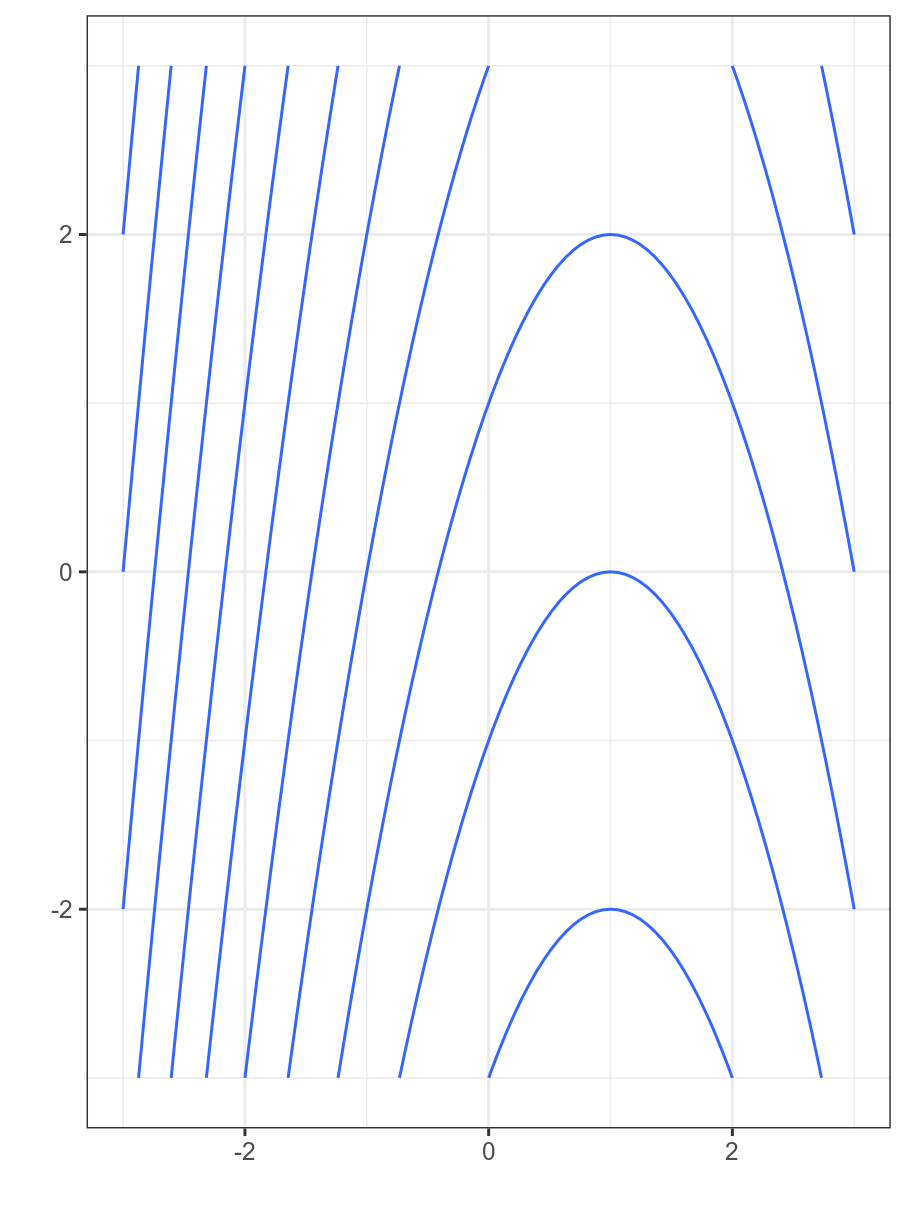
\includegraphics[scale = 0.3]{figure/line_curves.png}
% \begin{tikzpicture}[scale = 0.025]
%  % Created by tikzDevice version 0.12 on 2019-10-28 00:23:49
% !TEX encoding = UTF-8 Unicode
\definecolor{fillColor}{RGB}{255,255,255}
\path[use as bounding box,fill=fillColor,fill opacity=0.00] (0,0) rectangle (505.89,505.89);
\begin{scope}
\path[clip] (  0.00,  0.00) rectangle (505.89,505.89);
\definecolor{drawColor}{RGB}{255,255,255}
\definecolor{fillColor}{RGB}{255,255,255}

\path[draw=drawColor,line width= 0.6pt,line join=round,line cap=round,fill=fillColor] (  0.00,  0.00) rectangle (505.89,505.89);
\end{scope}
\begin{scope}
\path[clip] ( 30.10, 30.69) rectangle (500.39,500.39);
\definecolor{fillColor}{RGB}{255,255,255}

\path[fill=fillColor] ( 30.10, 30.69) rectangle (500.39,500.39);
\definecolor{drawColor}{gray}{0.92}

\path[draw=drawColor,line width= 0.3pt,line join=round] ( 30.10, 52.04) --
	(500.39, 52.04);

\path[draw=drawColor,line width= 0.3pt,line join=round] ( 30.10,194.37) --
	(500.39,194.37);

\path[draw=drawColor,line width= 0.3pt,line join=round] ( 30.10,336.71) --
	(500.39,336.71);

\path[draw=drawColor,line width= 0.3pt,line join=round] ( 30.10,479.04) --
	(500.39,479.04);

\path[draw=drawColor,line width= 0.3pt,line join=round] ( 51.47, 30.69) --
	( 51.47,500.39);

\path[draw=drawColor,line width= 0.3pt,line join=round] (193.99, 30.69) --
	(193.99,500.39);

\path[draw=drawColor,line width= 0.3pt,line join=round] (336.50, 30.69) --
	(336.50,500.39);

\path[draw=drawColor,line width= 0.3pt,line join=round] (479.01, 30.69) --
	(479.01,500.39);

\path[draw=drawColor,line width= 0.6pt,line join=round] ( 30.10,123.21) --
	(500.39,123.21);

\path[draw=drawColor,line width= 0.6pt,line join=round] ( 30.10,265.54) --
	(500.39,265.54);

\path[draw=drawColor,line width= 0.6pt,line join=round] ( 30.10,407.87) --
	(500.39,407.87);

\path[draw=drawColor,line width= 0.6pt,line join=round] (122.73, 30.69) --
	(122.73,500.39);

\path[draw=drawColor,line width= 0.6pt,line join=round] (265.24, 30.69) --
	(265.24,500.39);

\path[draw=drawColor,line width= 0.6pt,line join=round] (407.76, 30.69) --
	(407.76,500.39);
\definecolor{drawColor}{RGB}{51,102,255}

\path[draw=drawColor,line width= 0.6pt,line join=round] (265.28, 52.04) --
	(267.40, 56.29) --
	(267.44, 56.35) --
	(269.74, 60.67) --
	(271.72, 64.39) --
	(272.06, 64.98) --
	(274.51, 69.29) --
	(276.04, 71.97) --
	(277.04, 73.61) --
	(279.68, 77.92) --
	(280.36, 79.03) --
	(282.47, 82.23) --
	(284.68, 85.56) --
	(285.38, 86.54) --
	(288.48, 90.86) --
	(289.00, 91.58) --
	(291.82, 95.17) --
	(293.31, 97.07) --
	(295.42, 99.48) --
	(297.63,102.03) --
	(299.35,103.80) --
	(301.95,106.48) --
	(303.75,108.11) --
	(306.27,110.40) --
	(308.84,112.42) --
	(310.59,113.80) --
	(314.91,116.67) --
	(315.03,116.74) --
	(319.23,119.02) --
	(323.54,120.85) --
	(324.19,121.05) --
	(327.86,122.16) --
	(332.18,122.95) --
	(336.50,123.21) --
	(340.82,122.95) --
	(345.14,122.16) --
	(348.81,121.05) --
	(349.46,120.85) --
	(353.77,119.02) --
	(357.97,116.74) --
	(358.09,116.67) --
	(362.41,113.80) --
	(364.16,112.42) --
	(366.73,110.40) --
	(369.25,108.11) --
	(371.05,106.48) --
	(373.65,103.80) --
	(375.37,102.03) --
	(377.58, 99.48) --
	(379.69, 97.07) --
	(381.18, 95.17) --
	(384.00, 91.58) --
	(384.52, 90.86) --
	(387.62, 86.54) --
	(388.32, 85.56) --
	(390.53, 82.23) --
	(392.64, 79.03) --
	(393.32, 77.92) --
	(395.96, 73.61) --
	(396.96, 71.97) --
	(398.49, 69.29) --
	(400.94, 64.98) --
	(401.28, 64.39) --
	(403.26, 60.67) --
	(405.56, 56.35) --
	(405.60, 56.29) --
	(407.72, 52.04);

\path[draw=drawColor,line width= 0.6pt,line join=round] (213.10, 52.04) --
	(214.35, 56.35) --
	(215.58, 60.60) --
	(215.60, 60.67) --
	(216.90, 64.98) --
	(218.19, 69.29) --
	(219.49, 73.61) --
	(219.90, 74.98) --
	(220.82, 77.92) --
	(222.16, 82.23) --
	(223.50, 86.54) --
	(224.22, 88.83) --
	(224.87, 90.86) --
	(226.27, 95.17) --
	(227.67, 99.48) --
	(228.54,102.16) --
	(229.09,103.80) --
	(230.54,108.11) --
	(231.99,112.42) --
	(232.85,114.97) --
	(233.47,116.74) --
	(234.99,121.05) --
	(236.51,125.36) --
	(237.17,127.26) --
	(238.06,129.68) --
	(239.64,133.99) --
	(241.23,138.30) --
	(241.49,139.02) --
	(242.87,142.62) --
	(244.53,146.93) --
	(245.81,150.26) --
	(246.20,151.24) --
	(247.94,155.55) --
	(249.68,159.87) --
	(250.13,160.98) --
	(251.49,164.18) --
	(253.31,168.49) --
	(254.45,171.17) --
	(255.18,172.81) --
	(257.10,177.12) --
	(258.77,180.85) --
	(259.04,181.43) --
	(261.08,185.75) --
	(263.08,189.99) --
	(263.12,190.06) --
	(265.28,194.37) --
	(267.40,198.62) --
	(267.44,198.69) --
	(269.74,203.00) --
	(271.72,206.72) --
	(272.06,207.31) --
	(274.51,211.63) --
	(276.04,214.31) --
	(277.04,215.94) --
	(279.68,220.25) --
	(280.36,221.36) --
	(282.47,224.57) --
	(284.68,227.90) --
	(285.38,228.88) --
	(288.48,233.19) --
	(289.00,233.91) --
	(291.82,237.50) --
	(293.31,239.40) --
	(295.42,241.82) --
	(297.63,244.37) --
	(299.35,246.13) --
	(301.95,248.81) --
	(303.75,250.44) --
	(306.27,252.73) --
	(308.84,254.76) --
	(310.59,256.13) --
	(314.91,259.00) --
	(315.03,259.07) --
	(319.23,261.36) --
	(323.54,263.19) --
	(324.19,263.38) --
	(327.86,264.49) --
	(332.18,265.28) --
	(336.50,265.54) --
	(340.82,265.28) --
	(345.14,264.49) --
	(348.81,263.38) --
	(349.46,263.19) --
	(353.77,261.36) --
	(357.97,259.07) --
	(358.09,259.00) --
	(362.41,256.13) --
	(364.16,254.76) --
	(366.73,252.73) --
	(369.25,250.44) --
	(371.05,248.81) --
	(373.65,246.13) --
	(375.37,244.37) --
	(377.58,241.82) --
	(379.69,239.40) --
	(381.18,237.50) --
	(384.00,233.91) --
	(384.52,233.19) --
	(387.62,228.88) --
	(388.32,227.90) --
	(390.53,224.57) --
	(392.64,221.36) --
	(393.32,220.25) --
	(395.96,215.94) --
	(396.96,214.31) --
	(398.49,211.63) --
	(400.94,207.31) --
	(401.28,206.72) --
	(403.26,203.00) --
	(405.56,198.69) --
	(405.60,198.62) --
	(407.72,194.37) --
	(409.88,190.06) --
	(409.92,189.99) --
	(411.92,185.75) --
	(413.96,181.43) --
	(414.23,180.85) --
	(415.90,177.12) --
	(417.82,172.81) --
	(418.55,171.17) --
	(419.69,168.49) --
	(421.52,164.18) --
	(422.87,160.98) --
	(423.32,159.87) --
	(425.06,155.55) --
	(426.80,151.24) --
	(427.19,150.26) --
	(428.47,146.93) --
	(430.13,142.62) --
	(431.51,139.02) --
	(431.77,138.30) --
	(433.36,133.99) --
	(434.94,129.68) --
	(435.83,127.26) --
	(436.49,125.36) --
	(438.01,121.05) --
	(439.53,116.74) --
	(440.15,114.97) --
	(441.01,112.42) --
	(442.46,108.11) --
	(443.91,103.80) --
	(444.46,102.16) --
	(445.33, 99.48) --
	(446.73, 95.17) --
	(448.13, 90.86) --
	(448.78, 88.83) --
	(449.50, 86.54) --
	(450.84, 82.23) --
	(452.18, 77.92) --
	(453.10, 74.98) --
	(453.51, 73.61) --
	(454.81, 69.29) --
	(456.10, 64.98) --
	(457.40, 60.67) --
	(457.42, 60.60) --
	(458.65, 56.35) --
	(459.90, 52.04);

\path[draw=drawColor,line width= 0.6pt,line join=round] (177.17, 52.04) --
	(178.15, 56.35) --
	(179.12, 60.67) --
	(180.10, 64.98) --
	(181.03, 69.10) --
	(181.08, 69.29) --
	(182.08, 73.61) --
	(183.08, 77.92) --
	(184.09, 82.23) --
	(185.09, 86.54) --
	(185.35, 87.66) --
	(186.12, 90.86) --
	(187.15, 95.17) --
	(188.18, 99.48) --
	(189.21,103.80) --
	(189.67,105.69) --
	(190.26,108.11) --
	(191.33,112.42) --
	(192.39,116.74) --
	(193.46,121.05) --
	(193.99,123.21) --
	(194.54,125.36) --
	(195.63,129.68) --
	(196.73,133.99) --
	(197.82,138.30) --
	(198.31,140.20) --
	(198.94,142.62) --
	(200.07,146.93) --
	(201.20,151.24) --
	(202.33,155.55) --
	(202.62,156.67) --
	(203.49,159.87) --
	(204.66,164.18) --
	(205.83,168.49) --
	(206.94,172.61) --
	(207.00,172.81) --
	(208.21,177.12) --
	(209.41,181.43) --
	(210.62,185.75) --
	(211.26,188.03) --
	(211.85,190.06) --
	(213.10,194.37) --
	(214.35,198.69) --
	(215.58,202.93) --
	(215.60,203.00) --
	(216.90,207.31) --
	(218.19,211.63) --
	(219.49,215.94) --
	(219.90,217.31) --
	(220.82,220.25) --
	(222.16,224.57) --
	(223.50,228.88) --
	(224.22,231.17) --
	(224.87,233.19) --
	(226.27,237.50) --
	(227.67,241.82) --
	(228.54,244.50) --
	(229.09,246.13) --
	(230.54,250.44) --
	(231.99,254.76) --
	(232.85,257.31) --
	(233.47,259.07) --
	(234.99,263.38) --
	(236.51,267.70) --
	(237.17,269.59) --
	(238.06,272.01) --
	(239.64,276.32) --
	(241.23,280.64) --
	(241.49,281.35) --
	(242.87,284.95) --
	(244.53,289.26) --
	(245.81,292.59) --
	(246.20,293.58) --
	(247.94,297.89) --
	(249.68,302.20) --
	(250.13,303.31) --
	(251.49,306.51) --
	(253.31,310.83) --
	(254.45,313.51) --
	(255.18,315.14) --
	(257.10,319.45) --
	(258.77,323.18) --
	(259.04,323.77) --
	(261.08,328.08) --
	(263.08,332.33) --
	(263.12,332.39) --
	(265.28,336.71) --
	(267.40,340.95) --
	(267.44,341.02) --
	(269.74,345.33) --
	(271.72,349.06) --
	(272.06,349.65) --
	(274.51,353.96) --
	(276.04,356.64) --
	(277.04,358.27) --
	(279.68,362.59) --
	(280.36,363.70) --
	(282.47,366.90) --
	(284.68,370.23) --
	(285.38,371.21) --
	(288.48,375.52) --
	(289.00,376.24) --
	(291.82,379.84) --
	(293.31,381.73) --
	(295.42,384.15) --
	(297.63,386.70) --
	(299.35,388.46) --
	(301.95,391.14) --
	(303.75,392.78) --
	(306.27,395.06) --
	(308.84,397.09) --
	(310.59,398.46) --
	(314.91,401.34) --
	(315.03,401.40) --
	(319.23,403.69) --
	(323.54,405.52) --
	(324.19,405.72) --
	(327.86,406.83) --
	(332.18,407.61) --
	(336.50,407.87) --
	(340.82,407.61) --
	(345.14,406.83) --
	(348.81,405.72) --
	(349.46,405.52) --
	(353.77,403.69) --
	(357.97,401.40) --
	(358.09,401.34) --
	(362.41,398.46) --
	(364.16,397.09) --
	(366.73,395.06) --
	(369.25,392.78) --
	(371.05,391.14) --
	(373.65,388.46) --
	(375.37,386.70) --
	(377.58,384.15) --
	(379.69,381.73) --
	(381.18,379.84) --
	(384.00,376.24) --
	(384.52,375.52) --
	(387.62,371.21) --
	(388.32,370.23) --
	(390.53,366.90) --
	(392.64,363.70) --
	(393.32,362.59) --
	(395.96,358.27) --
	(396.96,356.64) --
	(398.49,353.96) --
	(400.94,349.65) --
	(401.28,349.06) --
	(403.26,345.33) --
	(405.56,341.02) --
	(405.60,340.95) --
	(407.72,336.71) --
	(409.88,332.39) --
	(409.92,332.33) --
	(411.92,328.08) --
	(413.96,323.77) --
	(414.23,323.18) --
	(415.90,319.45) --
	(417.82,315.14) --
	(418.55,313.51) --
	(419.69,310.83) --
	(421.52,306.51) --
	(422.87,303.31) --
	(423.32,302.20) --
	(425.06,297.89) --
	(426.80,293.58) --
	(427.19,292.59) --
	(428.47,289.26) --
	(430.13,284.95) --
	(431.51,281.35) --
	(431.77,280.64) --
	(433.36,276.32) --
	(434.94,272.01) --
	(435.83,269.59) --
	(436.49,267.70) --
	(438.01,263.38) --
	(439.53,259.07) --
	(440.15,257.31) --
	(441.01,254.76) --
	(442.46,250.44) --
	(443.91,246.13) --
	(444.46,244.50) --
	(445.33,241.82) --
	(446.73,237.50) --
	(448.13,233.19) --
	(448.78,231.17) --
	(449.50,228.88) --
	(450.84,224.57) --
	(452.18,220.25) --
	(453.10,217.31) --
	(453.51,215.94) --
	(454.81,211.63) --
	(456.10,207.31) --
	(457.40,203.00) --
	(457.42,202.93) --
	(458.65,198.69) --
	(459.90,194.37) --
	(461.15,190.06) --
	(461.74,188.03) --
	(462.38,185.75) --
	(463.59,181.43) --
	(464.79,177.12) --
	(466.00,172.81) --
	(466.06,172.61) --
	(467.17,168.49) --
	(468.34,164.18) --
	(469.51,159.87) --
	(470.38,156.67) --
	(470.67,155.55) --
	(471.80,151.24) --
	(472.93,146.93) --
	(474.06,142.62) --
	(474.69,140.20) --
	(475.18,138.30) --
	(476.27,133.99) --
	(477.37,129.68) --
	(478.46,125.36) --
	(479.01,123.21);

\path[draw=drawColor,line width= 0.6pt,line join=round] (147.98, 52.04) --
	(148.80, 56.35) --
	(149.62, 60.67) --
	(150.44, 64.98) --
	(150.80, 66.87) --
	(151.27, 69.29) --
	(152.11, 73.61) --
	(152.95, 77.92) --
	(153.79, 82.23) --
	(154.62, 86.54) --
	(155.12, 89.09) --
	(155.47, 90.86) --
	(156.33, 95.17) --
	(157.19, 99.48) --
	(158.05,103.80) --
	(158.91,108.11) --
	(159.44,110.79) --
	(159.77,112.42) --
	(160.65,116.74) --
	(161.53,121.05) --
	(162.41,125.36) --
	(163.29,129.68) --
	(163.76,131.96) --
	(164.18,133.99) --
	(165.08,138.30) --
	(165.98,142.62) --
	(166.89,146.93) --
	(167.79,151.24) --
	(168.08,152.61) --
	(168.71,155.55) --
	(169.63,159.87) --
	(170.56,164.18) --
	(171.48,168.49) --
	(172.39,172.74) --
	(172.41,172.81) --
	(173.36,177.12) --
	(174.31,181.43) --
	(175.26,185.75) --
	(176.21,190.06) --
	(176.71,192.35) --
	(177.17,194.37) --
	(178.15,198.69) --
	(179.12,203.00) --
	(180.10,207.31) --
	(181.03,211.43) --
	(181.08,211.63) --
	(182.08,215.94) --
	(183.08,220.25) --
	(184.09,224.57) --
	(185.09,228.88) --
	(185.35,229.99) --
	(186.12,233.19) --
	(187.15,237.50) --
	(188.18,241.82) --
	(189.21,246.13) --
	(189.67,248.03) --
	(190.26,250.44) --
	(191.33,254.76) --
	(192.39,259.07) --
	(193.46,263.38) --
	(193.99,265.54) --
	(194.54,267.70) --
	(195.63,272.01) --
	(196.73,276.32) --
	(197.82,280.64) --
	(198.31,282.53) --
	(198.94,284.95) --
	(200.07,289.26) --
	(201.20,293.58) --
	(202.33,297.89) --
	(202.62,299.00) --
	(203.49,302.20) --
	(204.66,306.51) --
	(205.83,310.83) --
	(206.94,314.94) --
	(207.00,315.14) --
	(208.21,319.45) --
	(209.41,323.77) --
	(210.62,328.08) --
	(211.26,330.37) --
	(211.85,332.39) --
	(213.10,336.71) --
	(214.35,341.02) --
	(215.58,345.27) --
	(215.60,345.33) --
	(216.90,349.65) --
	(218.19,353.96) --
	(219.49,358.27) --
	(219.90,359.64) --
	(220.82,362.59) --
	(222.16,366.90) --
	(223.50,371.21) --
	(224.22,373.50) --
	(224.87,375.52) --
	(226.27,379.84) --
	(227.67,384.15) --
	(228.54,386.83) --
	(229.09,388.46) --
	(230.54,392.78) --
	(231.99,397.09) --
	(232.85,399.64) --
	(233.47,401.40) --
	(234.99,405.72) --
	(236.51,410.03) --
	(237.17,411.93) --
	(238.06,414.34) --
	(239.64,418.66) --
	(241.23,422.97) --
	(241.49,423.69) --
	(242.87,427.28) --
	(244.53,431.60) --
	(245.81,434.93) --
	(246.20,435.91) --
	(247.94,440.22) --
	(249.68,444.53) --
	(250.13,445.65) --
	(251.49,448.85) --
	(253.31,453.16) --
	(254.45,455.84) --
	(255.18,457.47) --
	(257.10,461.79) --
	(258.77,465.51) --
	(259.04,466.10) --
	(261.08,470.41) --
	(263.08,474.66) --
	(263.12,474.73) --
	(265.28,479.04);

\path[draw=drawColor,line width= 0.6pt,line join=round] (479.01,265.54) --
	(478.46,267.70) --
	(477.37,272.01) --
	(476.27,276.32) --
	(475.18,280.64) --
	(474.69,282.53) --
	(474.06,284.95) --
	(472.93,289.26) --
	(471.80,293.58) --
	(470.67,297.89) --
	(470.38,299.00) --
	(469.51,302.20) --
	(468.34,306.51) --
	(467.17,310.83) --
	(466.06,314.94) --
	(466.00,315.14) --
	(464.79,319.45) --
	(463.59,323.77) --
	(462.38,328.08) --
	(461.74,330.37) --
	(461.15,332.39) --
	(459.90,336.71) --
	(458.65,341.02) --
	(457.42,345.27) --
	(457.40,345.33) --
	(456.10,349.65) --
	(454.81,353.96) --
	(453.51,358.27) --
	(453.10,359.64) --
	(452.18,362.59) --
	(450.84,366.90) --
	(449.50,371.21) --
	(448.78,373.50) --
	(448.13,375.52) --
	(446.73,379.84) --
	(445.33,384.15) --
	(444.46,386.83) --
	(443.91,388.46) --
	(442.46,392.78) --
	(441.01,397.09) --
	(440.15,399.64) --
	(439.53,401.40) --
	(438.01,405.72) --
	(436.49,410.03) --
	(435.83,411.93) --
	(434.94,414.34) --
	(433.36,418.66) --
	(431.77,422.97) --
	(431.51,423.69) --
	(430.13,427.28) --
	(428.47,431.60) --
	(427.19,434.93) --
	(426.80,435.91) --
	(425.06,440.22) --
	(423.32,444.53) --
	(422.87,445.65) --
	(421.52,448.85) --
	(419.69,453.16) --
	(418.55,455.84) --
	(417.82,457.47) --
	(415.90,461.79) --
	(414.23,465.51) --
	(413.96,466.10) --
	(411.92,470.41) --
	(409.92,474.66) --
	(409.88,474.73) --
	(407.72,479.04);

\path[draw=drawColor,line width= 0.6pt,line join=round] (122.74, 52.04) --
	(123.46, 56.35) --
	(124.18, 60.67) --
	(124.89, 64.91) --
	(124.90, 64.98) --
	(125.64, 69.29) --
	(126.37, 73.61) --
	(127.10, 77.92) --
	(127.84, 82.23) --
	(128.57, 86.54) --
	(129.21, 90.27) --
	(129.31, 90.86) --
	(130.06, 95.17) --
	(130.81, 99.48) --
	(131.56,103.80) --
	(132.31,108.11) --
	(133.06,112.42) --
	(133.53,115.10) --
	(133.82,116.74) --
	(134.58,121.05) --
	(135.35,125.36) --
	(136.12,129.68) --
	(136.88,133.99) --
	(137.65,138.30) --
	(137.85,139.41) --
	(138.43,142.62) --
	(139.21,146.93) --
	(139.99,151.24) --
	(140.78,155.55) --
	(141.56,159.87) --
	(142.16,163.20) --
	(142.35,164.18) --
	(143.15,168.49) --
	(143.95,172.81) --
	(144.75,177.12) --
	(145.55,181.43) --
	(146.35,185.75) --
	(146.48,186.47) --
	(147.17,190.06) --
	(147.98,194.37) --
	(148.80,198.69) --
	(149.62,203.00) --
	(150.44,207.31) --
	(150.80,209.21) --
	(151.27,211.63) --
	(152.11,215.94) --
	(152.95,220.25) --
	(153.79,224.57) --
	(154.62,228.88) --
	(155.12,231.43) --
	(155.47,233.19) --
	(156.33,237.50) --
	(157.19,241.82) --
	(158.05,246.13) --
	(158.91,250.44) --
	(159.44,253.12) --
	(159.77,254.76) --
	(160.65,259.07) --
	(161.53,263.38) --
	(162.41,267.70) --
	(163.29,272.01) --
	(163.76,274.30) --
	(164.18,276.32) --
	(165.08,280.64) --
	(165.98,284.95) --
	(166.89,289.26) --
	(167.79,293.58) --
	(168.08,294.95) --
	(168.71,297.89) --
	(169.63,302.20) --
	(170.56,306.51) --
	(171.48,310.83) --
	(172.39,315.08) --
	(172.41,315.14) --
	(173.36,319.45) --
	(174.31,323.77) --
	(175.26,328.08) --
	(176.21,332.39) --
	(176.71,334.68) --
	(177.17,336.71) --
	(178.15,341.02) --
	(179.12,345.33) --
	(180.10,349.65) --
	(181.03,353.76) --
	(181.08,353.96) --
	(182.08,358.27) --
	(183.08,362.59) --
	(184.09,366.90) --
	(185.09,371.21) --
	(185.35,372.32) --
	(186.12,375.52) --
	(187.15,379.84) --
	(188.18,384.15) --
	(189.21,388.46) --
	(189.67,390.36) --
	(190.26,392.78) --
	(191.33,397.09) --
	(192.39,401.40) --
	(193.46,405.72) --
	(193.99,407.87) --
	(194.54,410.03) --
	(195.63,414.34) --
	(196.73,418.66) --
	(197.82,422.97) --
	(198.31,424.86) --
	(198.94,427.28) --
	(200.07,431.60) --
	(201.20,435.91) --
	(202.33,440.22) --
	(202.62,441.33) --
	(203.49,444.53) --
	(204.66,448.85) --
	(205.83,453.16) --
	(206.94,457.28) --
	(207.00,457.47) --
	(208.21,461.79) --
	(209.41,466.10) --
	(210.62,470.41) --
	(211.26,472.70) --
	(211.85,474.73) --
	(213.10,479.04);

\path[draw=drawColor,line width= 0.6pt,line join=round] (479.01,407.87) --
	(478.46,410.03) --
	(477.37,414.34) --
	(476.27,418.66) --
	(475.18,422.97) --
	(474.69,424.86) --
	(474.06,427.28) --
	(472.93,431.60) --
	(471.80,435.91) --
	(470.67,440.22) --
	(470.38,441.33) --
	(469.51,444.53) --
	(468.34,448.85) --
	(467.17,453.16) --
	(466.06,457.28) --
	(466.00,457.47) --
	(464.79,461.79) --
	(463.59,466.10) --
	(462.38,470.41) --
	(461.74,472.70) --
	(461.15,474.73) --
	(459.90,479.04);

\path[draw=drawColor,line width= 0.6pt,line join=round] (100.18, 52.04) --
	(100.83, 56.35) --
	(101.48, 60.67) --
	(102.14, 64.98) --
	(102.79, 69.29) --
	(103.30, 72.63) --
	(103.45, 73.61) --
	(104.11, 77.92) --
	(104.78, 82.23) --
	(105.45, 86.54) --
	(106.11, 90.86) --
	(106.78, 95.17) --
	(107.44, 99.48) --
	(107.62,100.60) --
	(108.12,103.80) --
	(108.80,108.11) --
	(109.48,112.42) --
	(110.16,116.74) --
	(110.83,121.05) --
	(111.51,125.36) --
	(111.93,128.04) --
	(112.20,129.68) --
	(112.89,133.99) --
	(113.58,138.30) --
	(114.27,142.62) --
	(114.96,146.93) --
	(115.66,151.24) --
	(116.25,154.97) --
	(116.35,155.55) --
	(117.05,159.87) --
	(117.76,164.18) --
	(118.47,168.49) --
	(119.17,172.81) --
	(119.88,177.12) --
	(120.57,181.37) --
	(120.58,181.43) --
	(121.30,185.75) --
	(122.02,190.06) --
	(122.74,194.37) --
	(123.46,198.69) --
	(124.18,203.00) --
	(124.89,207.25) --
	(124.90,207.31) --
	(125.64,211.63) --
	(126.37,215.94) --
	(127.10,220.25) --
	(127.84,224.57) --
	(128.57,228.88) --
	(129.21,232.60) --
	(129.31,233.19) --
	(130.06,237.50) --
	(130.81,241.82) --
	(131.56,246.13) --
	(132.31,250.44) --
	(133.06,254.76) --
	(133.53,257.44) --
	(133.82,259.07) --
	(134.58,263.38) --
	(135.35,267.70) --
	(136.12,272.01) --
	(136.88,276.32) --
	(137.65,280.64) --
	(137.85,281.75) --
	(138.43,284.95) --
	(139.21,289.26) --
	(139.99,293.58) --
	(140.78,297.89) --
	(141.56,302.20) --
	(142.16,305.53) --
	(142.35,306.51) --
	(143.15,310.83) --
	(143.95,315.14) --
	(144.75,319.45) --
	(145.55,323.77) --
	(146.35,328.08) --
	(146.48,328.80) --
	(147.17,332.39) --
	(147.98,336.71) --
	(148.80,341.02) --
	(149.62,345.33) --
	(150.44,349.65) --
	(150.80,351.54) --
	(151.27,353.96) --
	(152.11,358.27) --
	(152.95,362.59) --
	(153.79,366.90) --
	(154.62,371.21) --
	(155.12,373.76) --
	(155.47,375.52) --
	(156.33,379.84) --
	(157.19,384.15) --
	(158.05,388.46) --
	(158.91,392.78) --
	(159.44,395.46) --
	(159.77,397.09) --
	(160.65,401.40) --
	(161.53,405.72) --
	(162.41,410.03) --
	(163.29,414.34) --
	(163.76,416.63) --
	(164.18,418.66) --
	(165.08,422.97) --
	(165.98,427.28) --
	(166.89,431.60) --
	(167.79,435.91) --
	(168.08,437.28) --
	(168.71,440.22) --
	(169.63,444.53) --
	(170.56,448.85) --
	(171.48,453.16) --
	(172.39,457.41) --
	(172.41,457.47) --
	(173.36,461.79) --
	(174.31,466.10) --
	(175.26,470.41) --
	(176.21,474.73) --
	(176.71,477.01) --
	(177.17,479.04);

\path[draw=drawColor,line width= 0.6pt,line join=round] ( 79.59, 52.04) --
	( 80.19, 56.35) --
	( 80.79, 60.67) --
	( 81.39, 64.98) --
	( 81.70, 67.27) --
	( 81.99, 69.29) --
	( 82.60, 73.61) --
	( 83.21, 77.92) --
	( 83.82, 82.23) --
	( 84.43, 86.54) --
	( 85.04, 90.86) --
	( 85.64, 95.17) --
	( 86.02, 97.85) --
	( 86.26, 99.48) --
	( 86.88,103.80) --
	( 87.50,108.11) --
	( 88.12,112.42) --
	( 88.74,116.74) --
	( 89.36,121.05) --
	( 89.98,125.36) --
	( 90.34,127.91) --
	( 90.60,129.68) --
	( 91.23,133.99) --
	( 91.86,138.30) --
	( 92.49,142.62) --
	( 93.12,146.93) --
	( 93.75,151.24) --
	( 94.38,155.55) --
	( 94.66,157.45) --
	( 95.02,159.87) --
	( 95.66,164.18) --
	( 96.30,168.49) --
	( 96.95,172.81) --
	( 97.59,177.12) --
	( 98.23,181.43) --
	( 98.87,185.75) --
	( 98.98,186.47) --
	( 99.52,190.06) --
	(100.18,194.37) --
	(100.83,198.69) --
	(101.48,203.00) --
	(102.14,207.31) --
	(102.79,211.63) --
	(103.30,214.96) --
	(103.45,215.94) --
	(104.11,220.25) --
	(104.78,224.57) --
	(105.45,228.88) --
	(106.11,233.19) --
	(106.78,237.50) --
	(107.44,241.82) --
	(107.62,242.93) --
	(108.12,246.13) --
	(108.80,250.44) --
	(109.48,254.76) --
	(110.16,259.07) --
	(110.83,263.38) --
	(111.51,267.70) --
	(111.93,270.38) --
	(112.20,272.01) --
	(112.89,276.32) --
	(113.58,280.64) --
	(114.27,284.95) --
	(114.96,289.26) --
	(115.66,293.58) --
	(116.25,297.30) --
	(116.35,297.89) --
	(117.05,302.20) --
	(117.76,306.51) --
	(118.47,310.83) --
	(119.17,315.14) --
	(119.88,319.45) --
	(120.57,323.70) --
	(120.58,323.77) --
	(121.30,328.08) --
	(122.02,332.39) --
	(122.74,336.71) --
	(123.46,341.02) --
	(124.18,345.33) --
	(124.89,349.58) --
	(124.90,349.65) --
	(125.64,353.96) --
	(126.37,358.27) --
	(127.10,362.59) --
	(127.84,366.90) --
	(128.57,371.21) --
	(129.21,374.94) --
	(129.31,375.52) --
	(130.06,379.84) --
	(130.81,384.15) --
	(131.56,388.46) --
	(132.31,392.78) --
	(133.06,397.09) --
	(133.53,399.77) --
	(133.82,401.40) --
	(134.58,405.72) --
	(135.35,410.03) --
	(136.12,414.34) --
	(136.88,418.66) --
	(137.65,422.97) --
	(137.85,424.08) --
	(138.43,427.28) --
	(139.21,431.60) --
	(139.99,435.91) --
	(140.78,440.22) --
	(141.56,444.53) --
	(142.16,447.87) --
	(142.35,448.85) --
	(143.15,453.16) --
	(143.95,457.47) --
	(144.75,461.79) --
	(145.55,466.10) --
	(146.35,470.41) --
	(146.48,471.13) --
	(147.17,474.73) --
	(147.98,479.04);

\path[draw=drawColor,line width= 0.6pt,line join=round] ( 60.53, 52.04) --
	( 61.09, 56.35) --
	( 61.65, 60.67) --
	( 62.21, 64.98) --
	( 62.77, 69.29) --
	( 63.33, 73.61) --
	( 63.89, 77.92) --
	( 64.43, 82.04) --
	( 64.46, 82.23) --
	( 65.03, 86.54) --
	( 65.60, 90.86) --
	( 66.17, 95.17) --
	( 66.74, 99.48) --
	( 67.31,103.80) --
	( 67.88,108.11) --
	( 68.45,112.42) --
	( 68.75,114.71) --
	( 69.02,116.74) --
	( 69.60,121.05) --
	( 70.18,125.36) --
	( 70.76,129.68) --
	( 71.34,133.99) --
	( 71.92,138.30) --
	( 72.50,142.62) --
	( 73.07,146.86) --
	( 73.08,146.93) --
	( 73.66,151.24) --
	( 74.25,155.55) --
	( 74.84,159.87) --
	( 75.43,164.18) --
	( 76.02,168.49) --
	( 76.61,172.81) --
	( 77.20,177.12) --
	( 77.39,178.49) --
	( 77.79,181.43) --
	( 78.39,185.75) --
	( 78.99,190.06) --
	( 79.59,194.37) --
	( 80.19,198.69) --
	( 80.79,203.00) --
	( 81.39,207.31) --
	( 81.70,209.60) --
	( 81.99,211.63) --
	( 82.60,215.94) --
	( 83.21,220.25) --
	( 83.82,224.57) --
	( 84.43,228.88) --
	( 85.04,233.19) --
	( 85.64,237.50) --
	( 86.02,240.18) --
	( 86.26,241.82) --
	( 86.88,246.13) --
	( 87.50,250.44) --
	( 88.12,254.76) --
	( 88.74,259.07) --
	( 89.36,263.38) --
	( 89.98,267.70) --
	( 90.34,270.25) --
	( 90.60,272.01) --
	( 91.23,276.32) --
	( 91.86,280.64) --
	( 92.49,284.95) --
	( 93.12,289.26) --
	( 93.75,293.58) --
	( 94.38,297.89) --
	( 94.66,299.78) --
	( 95.02,302.20) --
	( 95.66,306.51) --
	( 96.30,310.83) --
	( 96.95,315.14) --
	( 97.59,319.45) --
	( 98.23,323.77) --
	( 98.87,328.08) --
	( 98.98,328.80) --
	( 99.52,332.39) --
	(100.18,336.71) --
	(100.83,341.02) --
	(101.48,345.33) --
	(102.14,349.65) --
	(102.79,353.96) --
	(103.30,357.29) --
	(103.45,358.27) --
	(104.11,362.59) --
	(104.78,366.90) --
	(105.45,371.21) --
	(106.11,375.52) --
	(106.78,379.84) --
	(107.44,384.15) --
	(107.62,385.26) --
	(108.12,388.46) --
	(108.80,392.78) --
	(109.48,397.09) --
	(110.16,401.40) --
	(110.83,405.72) --
	(111.51,410.03) --
	(111.93,412.71) --
	(112.20,414.34) --
	(112.89,418.66) --
	(113.58,422.97) --
	(114.27,427.28) --
	(114.96,431.60) --
	(115.66,435.91) --
	(116.25,439.63) --
	(116.35,440.22) --
	(117.05,444.53) --
	(117.76,448.85) --
	(118.47,453.16) --
	(119.17,457.47) --
	(119.88,461.79) --
	(120.57,466.04) --
	(120.58,466.10) --
	(121.30,470.41) --
	(122.02,474.73) --
	(122.74,479.04);

\path[draw=drawColor,line width= 0.6pt,line join=round] ( 51.47,123.21) --
	( 51.75,125.36) --
	( 52.29,129.68) --
	( 52.83,133.99) --
	( 53.38,138.30) --
	( 53.92,142.62) --
	( 54.47,146.93) --
	( 55.01,151.24) --
	( 55.55,155.55) --
	( 55.79,157.45) --
	( 56.10,159.87) --
	( 56.65,164.18) --
	( 57.21,168.49) --
	( 57.76,172.81) --
	( 58.31,177.12) --
	( 58.86,181.43) --
	( 59.42,185.75) --
	( 59.97,190.06) --
	( 60.11,191.17) --
	( 60.53,194.37) --
	( 61.09,198.69) --
	( 61.65,203.00) --
	( 62.21,207.31) --
	( 62.77,211.63) --
	( 63.33,215.94) --
	( 63.89,220.25) --
	( 64.43,224.37) --
	( 64.46,224.57) --
	( 65.03,228.88) --
	( 65.60,233.19) --
	( 66.17,237.50) --
	( 66.74,241.82) --
	( 67.31,246.13) --
	( 67.88,250.44) --
	( 68.45,254.76) --
	( 68.75,257.04) --
	( 69.02,259.07) --
	( 69.60,263.38) --
	( 70.18,267.70) --
	( 70.76,272.01) --
	( 71.34,276.32) --
	( 71.92,280.64) --
	( 72.50,284.95) --
	( 73.07,289.20) --
	( 73.08,289.26) --
	( 73.66,293.58) --
	( 74.25,297.89) --
	( 74.84,302.20) --
	( 75.43,306.51) --
	( 76.02,310.83) --
	( 76.61,315.14) --
	( 77.20,319.45) --
	( 77.39,320.83) --
	( 77.79,323.77) --
	( 78.39,328.08) --
	( 78.99,332.39) --
	( 79.59,336.71) --
	( 80.19,341.02) --
	( 80.79,345.33) --
	( 81.39,349.65) --
	( 81.70,351.93) --
	( 81.99,353.96) --
	( 82.60,358.27) --
	( 83.21,362.59) --
	( 83.82,366.90) --
	( 84.43,371.21) --
	( 85.04,375.52) --
	( 85.64,379.84) --
	( 86.02,382.52) --
	( 86.26,384.15) --
	( 86.88,388.46) --
	( 87.50,392.78) --
	( 88.12,397.09) --
	( 88.74,401.40) --
	( 89.36,405.72) --
	( 89.98,410.03) --
	( 90.34,412.58) --
	( 90.60,414.34) --
	( 91.23,418.66) --
	( 91.86,422.97) --
	( 92.49,427.28) --
	( 93.12,431.60) --
	( 93.75,435.91) --
	( 94.38,440.22) --
	( 94.66,442.12) --
	( 95.02,444.53) --
	( 95.66,448.85) --
	( 96.30,453.16) --
	( 96.95,457.47) --
	( 97.59,461.79) --
	( 98.23,466.10) --
	( 98.87,470.41) --
	( 98.98,471.13) --
	( 99.52,474.73) --
	(100.18,479.04);

\path[draw=drawColor,line width= 0.6pt,line join=round] ( 51.47,265.54) --
	( 51.75,267.70) --
	( 52.29,272.01) --
	( 52.83,276.32) --
	( 53.38,280.64) --
	( 53.92,284.95) --
	( 54.47,289.26) --
	( 55.01,293.58) --
	( 55.55,297.89) --
	( 55.79,299.78) --
	( 56.10,302.20) --
	( 56.65,306.51) --
	( 57.21,310.83) --
	( 57.76,315.14) --
	( 58.31,319.45) --
	( 58.86,323.77) --
	( 59.42,328.08) --
	( 59.97,332.39) --
	( 60.11,333.50) --
	( 60.53,336.71) --
	( 61.09,341.02) --
	( 61.65,345.33) --
	( 62.21,349.65) --
	( 62.77,353.96) --
	( 63.33,358.27) --
	( 63.89,362.59) --
	( 64.43,366.70) --
	( 64.46,366.90) --
	( 65.03,371.21) --
	( 65.60,375.52) --
	( 66.17,379.84) --
	( 66.74,384.15) --
	( 67.31,388.46) --
	( 67.88,392.78) --
	( 68.45,397.09) --
	( 68.75,399.38) --
	( 69.02,401.40) --
	( 69.60,405.72) --
	( 70.18,410.03) --
	( 70.76,414.34) --
	( 71.34,418.66) --
	( 71.92,422.97) --
	( 72.50,427.28) --
	( 73.07,431.53) --
	( 73.08,431.60) --
	( 73.66,435.91) --
	( 74.25,440.22) --
	( 74.84,444.53) --
	( 75.43,448.85) --
	( 76.02,453.16) --
	( 76.61,457.47) --
	( 77.20,461.79) --
	( 77.39,463.16) --
	( 77.79,466.10) --
	( 78.39,470.41) --
	( 78.99,474.73) --
	( 79.59,479.04);

\path[draw=drawColor,line width= 0.6pt,line join=round] ( 51.47,407.87) --
	( 51.75,410.03) --
	( 52.29,414.34) --
	( 52.83,418.66) --
	( 53.38,422.97) --
	( 53.92,427.28) --
	( 54.47,431.60) --
	( 55.01,435.91) --
	( 55.55,440.22) --
	( 55.79,442.12) --
	( 56.10,444.53) --
	( 56.65,448.85) --
	( 57.21,453.16) --
	( 57.76,457.47)
%  \end{tikzpicture}
  \end{center}
\end{minipage}
  


\item Find the local maxima and minima of the function $f(x,y)=x^4+2y^4-xy$. Determine whether the extrema you have found are global or local.

\item Find the gradient of the function $h(x,y)=f(x,y)\cdot g(x,y)$ at the point $A=(1,7)$. It is known that at the point $A$: $\grad f=(1,1)$, $\grad g=(3,3)$, $f(A)=4$, $g(A)=5$.

\item Consider the following system of equations as defining functions $y_1(x_1,x_2)$ and $y_2(x_1,x_2)$
\[
\left\{
\begin{array}{c}
x_1^3+x_1 y_1^3+x_2 y_1 y_2+y_2^3=4 \\
x_2+x_2^3+y_1 y_2^2+y_2^3=4
\end{array}
\right.
\]
\begin{enumerate}
\item If possible find $dy_1$ at the point $(x_1,x_2,y_1,y_2)=(1,1,1,1)$.
\item Find approximately $y_1$ for $x_1=1.01$ and $x_2=0.98$.
\end{enumerate}
\item Find the constrained extrema of the function $f(x,y)=x+2y$ subject to $2x^2+y^2=10$.
%Short run total costs are given by $TC(q,K)=q^2+3qK+4K^2-2K$ where $q$ is the volume of output and $K$ is the amount of capital which is fixed in the short run. In the long run the firm can adapt the amount of $K$ to minimize the costs. Find the long run marginal costs using envelope theorem.

\item Find the Hesse matrix of the function $h(x,y)=\P( Z \in [2x;3y])$ where $Z$ is a standard normal random variable with probability density function given by $f(z)=\frac{1}{\sqrt{2\pi}}\exp(-z^2/2)$. It is supposed that $3y>2x$.

\end{enumerate}

\textbf{SECTION B:}
\begin{enumerate}
\item A firm’s production function is $Q=K+L+2\sqrt{KL}$, where $K>0$ and $L>0$ are capital and labor, respectively. The firm is perfectly competitive and seeks to maximize its output, but the firm is run by accountants who have imposed a fixed budget on the production of $C$ dollars per hour, which means satisfying constraint $wL+rK=C$, where $w$ and $r$ are hourly wage rate and rental rate of capital, respectively.
\begin{enumerate}
\item State the constrained optimization problem associated with that production and solve it by the Lagrange multiplier method (it is sufficient to find the optimal values of capital and labor alone).
\item Check the concavity of the production function and use it to classify the critical point.
\item Explain the economic meaning of the Lagrange multiplier in this problem. Use the appropriate envelope theorem.
\item Let $w=r$. Would it be right to conclude that if the wage rate goes up by 1\% and the rental rate goes down by the same 1\% under the fixed budget the output will not change?  How can you prove this mathematically?
\end{enumerate}

\item It is well known that a perfectly competitive firm operating in the long-run produces at the minimum point of its average costs curve, where $p=AC=MC$. Let the $AC$ curve be U-shaped. If we assume that this particular firm uses only labor, equation $AC(y,w)=MC(y,w)$ may be used to find $y=y(w)$  as an implicit function of wages ($y$ denotes the output). Moreover, the second-order condition that guarantees the profit maximization is supposed to hold.
\begin{enumerate}
\item Show that Implicit Function Theorem can be applied, the function $y=y(w)$ exists and find its derivative.
\item If we know that at long-run equilibrium $\frac{\partial MC}{\partial w}>\frac{\partial AC}{\partial w}$  what can we say about new long-run equilibrium when the market adjusts to a small rise in wage $w$? Will the equilibrium price go up? What about the output of the firm?
\end{enumerate}
\end{enumerate}

\subsection{MFE, fall retake 23.01.13}

Part A, 10 points for each problem.

\vspace{20pt}

\begin{enumerate}
\item It is known that $f'_x(x,y)>0$ and $f'_y(x,y)>0$. Sketch possible level curves for $f(x,y)$. What are the possible values of the angle between the gradient of the function $f$ and the $x$-axis?
\item Find the local maxima and minima of the function $f(x,y)=x^4+4y^4-xy$. Determine whether the extrema you have found are global or local.
\item Find and classify the constrained extrema of the function $f(x,y)=x+5y$ subject to $2x^2+y^2=10$.

\item Given the system
\[
\begin{cases}
xe^{u+v}+2uv=1 \\
ye^{u-v}-\frac{u}{1+v}=2x
\end{cases}
\]
find $du$ and $dv$ at $x_0 = 1$, $y_0 = 2$, $u_0 = 0$, $v_0 = 0$.

\item Find the total differential for the function $f(x,y)=x^2y^2+xy^2+2x+4y$. Using the total differential find approximately $f(1.001,1.999)$

\item Use the chain rule to find $f'(x)$ and $f''(x)$ for $f(x)=u(a,b,x)$ where $a=\cos(x)$ and $b=x^3$.

\end{enumerate}

\vspace{20pt}

Part B, 20 points for each problem.

\vspace{20pt}

\begin{enumerate}[resume]
\item A consumer maximizes the quasilinear utility function $u(x,y)=v(x)+y$, where $v'>0$, $v''<0$, subject to the budget constraint $px+y=I$.
\begin{enumerate}
\item (10 points) Denote the demand on $x$ by $x^*$. Show that $\frac{\partial x^*}{\partial I}=0$ and $\frac{\partial x^*}{\partial p}<0$.
\item (10 points) Let $V=u(x^*,y^*)$, where $(x^*,y^*)$ is the optimal bundle. Assuming that $y^*>0$ and using the appropriate envelope theorem, show that $\frac{\partial V}{\partial I}$ is constant.
\end{enumerate}

\item A two-product firm produces outputs $y_1$ and $y_2$ from a single factor of production which is labor, in other words, there is a function $f$, such that $f(y_1,y_2)\leq \bar{L}$. Output prices are $p_1$ and $p_2$. The firm has a fixed amount of labor supply $\bar{L}>0$ that should be utilized in full.
\begin{enumerate}
\item (10 points) Set the problem of the revenue maximization under the labor constraint mathematically and derive first-order conditions. Assume that both outputs should be produced in positive amounts.
\item (10 points) Let the maximum value of the total revenue under the labor constraint be $TR(p_1,p_2,\bar{L})$. What are its derivatives with respect to the prices?
\end{enumerate}

\end{enumerate}

\subsection{MFE, mock, 28.03.2013}

Marks will be deducted for insufficient explanation within your answers. All problems are mandatory. Sections A and B will make up 60\% and 40\% of the exam grade, respectively. Total duration of the exam is 120 min. \\

\textbf{SECTION A}
\vspace{20pt}

\begin{enumerate}

\item Compute all the roots of the complex number, $\sqrt[5]{-1+i}$

\item The matrix $A$ has the eigenvalues $\lambda_1=-1$, $\lambda_2=3$, $\lambda_3=-2$.
\begin{enumerate}
\item Compute the eigenvalues of the following matrices: $B=A^2$, $C=A+3I$, $D=A^{-1}$ where $I$ is the corresponding identity matrix.
\item What can be said about the definiteness of these matrices?
\end{enumerate}

\item Consider the implicit function $y(x)$ given by the equation
\[
y^3+y+3x^3+x^2=14.
\]
\begin{enumerate}
\item Does this equation define the implicit function $y(x)$ in the neighborhood of the point $(1,2)$?
\item If the implicit function is defined find the Taylor series for $y(x)$ up to the second order term.
\end{enumerate}


\item Consider the difference equation $y_{t+1}(2+3y_t)=4y_t$ with initial condition $y_0=2/3$.
\begin{enumerate}
\item Using the substitution $z_t=1/y_t$ solve the difference equation.
\item What is the limit of $y_t$ as $t\to\infty$?
\end{enumerate}

\item The homogeneous function $f$ is given by the equation
\[
f(x,y)=\int_0^{xy^a} t^3+xt \, dt.
\]
Find the value of the parameter $a$ and the degree of homogeneity of $\partial f/\partial x$.

\item Find the two indefinite integrals $\int e^x \cos(2x)\,dx$, $\int \frac{x+1}{x^2-5x+4}\, dx$

\end{enumerate}

\vspace{20pt}
\textbf{SECTION B}
\vspace{20pt}

\begin{enumerate}[resume]
\item Suppose you enter a casino with $k$ dollars in your pocket. You decide to play a game in which you win \$1 with the probability  $2/3$ and lose \$1 dollar with the probability $1/3$. The game is over when $k=0$ (no money left) or $k=100$.

Denote the probability to win the game, i.e. reaching $k=100$, starting with $k$ dollars as $x_k=\P(win|k)$. Using the total probability formula
\[
\P(win|k)=\frac{1}{3} \cdot \P(win|k-1)+\frac{2}{3} \cdot \P(win|k+1)
\]
derive the difference equation for $x_k$ and solve the boundary-value problem with $x_0=0$ and $x_{100}=1$.

\item Let $N(t)$ denote the size of population, $X(t)=\sqrt{N}$ the total output in the economy. Consider the following model
\[
\frac{\dot{N}}{N}=\alpha-\beta\frac{N}{X}
\]
where $\alpha>0$, $\beta>0$. Find $N$ and explore its behavior as $t\to\infty$.
\end{enumerate}

% more variants :)
\begin{comment}

\newpage
\pagestyle{empty}
Mathematics for economists. Exam Paper. March 28, 2013, \textbf{Variant 2} \\

%Lecturer: K.A. Bukin
%Class teachers: A. Arlashin, G. Sharygin, S. Provornikov

Marks will be deducted for insufficient explanation within your answers. All problems are mandatory. Sections A and B will make up 60\% and 40\% of the exam grade, respectively. Total duration of the exam is 120 min. \\

\textbf{SECTION A}
\vspace{20pt}

\begin{enumerate}

\item Compute all the roots of the complex number, $\sqrt[5]{-1-i}$

\item The matrix $A$ has the eigenvalues $\lambda_1=-1$, $\lambda_2=4$, $\lambda_3=-2$.
\begin{enumerate}
\item Compute the eigenvalues of the following matrices: $B=A^2$, $C=A+3I$, $D=A^{-1}$ where $I$ is the corresponding identity matrix.
\item What can be said about the definiteness of these matrices?
\end{enumerate}

\item Consider the implicit function $y(x)$ given by the equation
\[
y^3+2y+3x^3+x^2=16.
\]
\begin{enumerate}
\item Does this equation define the implicit function $y(x)$ in the neighborhood of the point $(1,2)$?
\item If the implicit function is defined find the Taylor series for $y(x)$ up to the second order term.
\end{enumerate}


\item Consider the difference equation $y_{t+1}(2+3y_t)=4y_t$ with initial condition $y_0=2/3$.
\begin{enumerate}
\item Using the substitution $z_t=1/y_t$ solve the difference equation.
\item What is the limit of $y_t$ as $t\to\infty$?
\end{enumerate}

\item The homogeneous function $f$ is given by the equation
\[
f(x,y)=\int_0^{xy^a} t^3+xt \, dt.
\]
Find the value of the parameter $a$ and the degree of homogeneity of $\partial f/\partial x$.

\item Find the two indefinite integrals $\int e^x \cos(3x)\,dx$, $\int \frac{x+2}{x^2-5x+4}\, dx$

\end{enumerate}

\vspace{20pt}
\textbf{SECTION B}
\vspace{20pt}

\begin{enumerate}[resume]
\item Suppose you enter a casino with $k$ dollars in your pocket. You decide to play a game in which you win \$1 with the probability  $2/3$ and lose \$1 dollar with the probability $1/3$. The game is over when $k=0$ (no money left) or $k=100$.

Denote the probability to win the game, i.e. reaching $k=100$, starting with $k$ dollars as $x_k=\P(win|k)$. Using the total probability formula
\[
\P(win|k)=\frac{1}{3} \cdot \P(win|k-1)+\frac{2}{3} \cdot \P(win|k+1)
\]
derive the difference equation for $x_k$ and solve the boundary-value problem with $x_0=0$ and $x_{100}=1$.

\item Let $N(t)$ denote the size of population, $X(t)=\sqrt{N}$ the total output in the economy. Consider the following model
\[
\frac{\dot{N}}{N}=\alpha-\beta\frac{N}{X}
\]
where $\alpha>0$, $\beta>0$. Find $N$ and explore its behavior as $t\to\infty$.
\end{enumerate}


\newpage
\pagestyle{empty}
Mathematics for economists. Exam Paper. March 28, 2013, \textbf{Variant 3} \\

%Lecturer: K.A. Bukin
%Class teachers: A. Arlashin, G. Sharygin, S. Provornikov

Marks will be deducted for insufficient explanation within your answers. All problems are mandatory. Sections A and B will make up 60\% and 40\% of the exam grade, respectively. Total duration of the exam is 120 min. \\

\textbf{SECTION A}
\vspace{20pt}

\begin{enumerate}

\item Compute all the roots of the complex number, $\sqrt[5]{1-i}$

\item The matrix $A$ has the eigenvalues $\lambda_1=-1$, $\lambda_2=5$, $\lambda_3=-2$.
\begin{enumerate}
\item Compute the eigenvalues of the following matrices: $B=A^2$, $C=A+3I$, $D=A^{-1}$ where $I$ is the corresponding identity matrix.
\item What can be said about the definiteness of these matrices?
\end{enumerate}

\item Consider the implicit function $y(x)$ given by the equation
\[
y^3+3y+3x^3+x^2=18.
\]
\begin{enumerate}
\item Does this equation define the implicit function $y(x)$ in the neighborhood of the point $(1,2)$?
\item If the implicit function is defined find the Taylor series for $y(x)$ up to the second order term.
\end{enumerate}


\item Consider the difference equation $y_{t+1}(2+3y_t)=4y_t$ with initial condition $y_0=2/3$.
\begin{enumerate}
\item Using the substitution $z_t=1/y_t$ solve the difference equation.
\item What is the limit of $y_t$ as $t\to\infty$?
\end{enumerate}

\item The homogeneous function $f$ is given by the equation
\[
f(x,y)=\int_0^{xy^a} t^3+xt \, dt.
\]
Find the value of the parameter $a$ and the degree of homogeneity of $\partial f/\partial x$.

\item Find the two indefinite integrals $\int e^x \cos(4x)\,dx$, $\int \frac{x+3}{x^2-5x+4}\, dx$

\end{enumerate}

\vspace{20pt}
\textbf{SECTION B}
\vspace{20pt}

\begin{enumerate}[resume]
\item Suppose you enter a casino with $k$ dollars in your pocket. You decide to play a game in which you win \$1 with the probability  $2/3$ and lose \$1 dollar with the probability $1/3$. The game is over when $k=0$ (no money left) or $k=100$.

Denote the probability to win the game, i.e. reaching $k=100$, starting with $k$ dollars as $x_k=\P(win|k)$. Using the total probability formula
\[
\P(win|k)=\frac{1}{3} \cdot \P(win|k-1)+\frac{2}{3} \cdot \P(win|k+1)
\]
derive the difference equation for $x_k$ and solve the boundary-value problem with $x_0=0$ and $x_{100}=1$.

\item Let $N(t)$ denote the size of population, $X(t)=\sqrt{N}$ the total output in the economy. Consider the following model
\[
\frac{\dot{N}}{N}=\alpha-\beta\frac{N}{X}
\]
where $\alpha>0$, $\beta>0$. Find $N$ and explore its behavior as $t\to\infty$.
\end{enumerate}


\newpage
\pagestyle{empty}
Mathematics for economists. Exam Paper. March 28, 2013, \textbf{Variant 4} \\

%Lecturer: K.A. Bukin
%Class teachers: A. Arlashin, G. Sharygin, S. Provornikov

Marks will be deducted for insufficient explanation within your answers. All problems are mandatory. Sections A and B will make up 60\% and 40\% of the exam grade, respectively. Total duration of the exam is 120 min. \\

\textbf{SECTION A}
\vspace{20pt}

\begin{enumerate}

\item Compute all the roots of the complex number, $\sqrt[5]{1+i}$

\item The matrix $A$ has the eigenvalues $\lambda_1=-1$, $\lambda_2=6$, $\lambda_3=-2$.
\begin{enumerate}
\item Compute the eigenvalues of the following matrices: $B=A^2$, $C=A+3I$, $D=A^{-1}$ where $I$ is the corresponding identity matrix.
\item What can be said about the definiteness of these matrices?
\end{enumerate}

\item Consider the implicit function $y(x)$ given by the equation
\[
y^3+4y+3x^3+x^2=20.
\]
\begin{enumerate}
\item Does this equation define the implicit function $y(x)$ in the neighborhood of the point $(1,2)$?
\item If the implicit function is defined find the Taylor series for $y(x)$ up to the second order term.
\end{enumerate}


\item Consider the difference equation $y_{t+1}(2+3y_t)=4y_t$ with initial condition $y_0=2/3$.
\begin{enumerate}
\item Using the substitution $z_t=1/y_t$ solve the difference equation.
\item What is the limit of $y_t$ as $t\to\infty$?
\end{enumerate}

\item The homogeneous function $f$ is given by the equation
\[
f(x,y)=\int_0^{xy^a} t^3+xt \, dt.
\]
Find the value of the parameter $a$ and the degree of homogeneity of $\partial f/\partial x$.

\item Find the two indefinite integrals $\int e^x \cos(5x)\,dx$, $\int \frac{x+4}{x^2-5x+4}\, dx$

\end{enumerate}

\vspace{20pt}
\textbf{SECTION B}
\vspace{20pt}

\begin{enumerate}[resume]
\item Suppose you enter a casino with $k$ dollars in your pocket. You decide to play a game in which you win \$1 with the probability  $2/3$ and lose \$1 dollar with the probability $1/3$. The game is over when $k=0$ (no money left) or $k=100$.

Denote the probability to win the game, i.e. reaching $k=100$, starting with $k$ dollars as $x_k=\P(win|k)$. Using the total probability formula
\[
\P(win|k)=\frac{1}{3} \cdot \P(win|k-1)+\frac{2}{3} \cdot \P(win|k+1)
\]
derive the difference equation for $x_k$ and solve the boundary-value problem with $x_0=0$ and $x_{100}=1$.

\item Let $N(t)$ denote the size of population, $X(t)=\sqrt{N}$ the total output in the economy. Consider the following model
\[
\frac{\dot{N}}{N}=\alpha-\beta\frac{N}{X}
\]
where $\alpha>0$, $\beta>0$. Find $N$ and explore its behavior as $t\to\infty$.
\end{enumerate}
\end{comment}

\subsection{MOR, exam, 22.05.2013}


You need to solve exactly FIVE problems out of 7. At least ONE problem from each section should be chosen for solving. Each question is worth 20 points.

\vspace{20pt}
\textbf{SECTION A}
\vspace{20pt}

\begin{enumerate}
\item A two-product monopoly seeks to maximize its profit. The revenue  follows the formula $R(x,y)=6x-x^2+y-y^2$. The total costs function is given by $C(x,y)=x^2+y^2+4x+3y$, where $x$ and $y$ are the outputs.

State the problem of the monopoly, given condition that its profit $\pi=R-C$ should always remain nonnegative. Apply the Kuhn-Tucker conditions. Use Weierstrass theorem to confirm sufficiency.
\item For any real number $\lambda$, find the minimal value of the objective function $x_1+6x_2+2x_3+4x_4$ subject to the constraints  $\lambda x_1+x_2-x_3+x_4\geq -1$, $x_1+1.5x_2+x_3+x_4 \geq 5$,  all choice variables are nonnegative.
\end{enumerate}

\vspace{20pt}
\textbf{SECTION B}
\vspace{20pt}

\begin{enumerate}[resume]
\item Solve the system of differential equations:
\[
\begin{cases}
\dot{x}=x-y \\
\dot{y}=2x-y
\end{cases}
\]
\item Given the Metzler equation of inventory cycles $y_t=3by_{t-1}-2by_{t-2}+N$, where $0<b<1$ and $N$ is a number, find all such values of $b$ for which solution represents convergent stepped time path (the complex roots case). Does the value of $N$ affect your conclusion?
\item Show that Chebyshev’s equation $(1-x^2)y''-xy'+y=0$, where $|x|<1$, can be reduced to equation $\ddot{y}+y=0$ by substituting $x=\cos t$. Hence find the general solution of Chebyshev’s equation.
\end{enumerate}

\vspace{20pt}
\textbf{SECTION C}
\vspace{20pt}

\begin{enumerate}[resume]
\item Find all pure and mixed Nash equilibria in the following bimatrix game:


\begin{tabular}{c|ccc}
 & d & e & f \\
\hline
a & 4;5 & 1;4 & 1;1  \\
b & 2;8 & 5;0 & 0;4  \\
c & 0;3 & 2;2 & 5;7  \\
\end{tabular}


\item There is an auction of a painting with two players. The value of the painting for the first player is a random variable $v_1$, for the second player --- $v_2$. The random variables $v_1$ and $v_2$ are independent and uniformly distributed from 0 to 1 million dollars. Each player makes the bid $b_i$ knowing only his own value of the painting. The player who makes the highest bid gets the painting and pays the arithmetic mean of the two bids.

Find a Nash equilibrium where each player uses linear strategy of the form $b_i=k\cdot v_i$.

\end{enumerate}

\subsection{MOR, marking scheme, 22.05.2013 }

\begin{enumerate}
\item 5 points for setting Kuhn-Tucker Lagrangian correctly and writing down first-order conditions. Another 3 points for showing that the only constraint in the problem is binding. 5 points for proving that an internal  critical point ($x>0$, $y>0$) does not exist. Plus 3 points for finding corner critical point. And 4 points for showing that Weierstrass theorem is applicable.

\item 10 points for conversion to the dual program and correct analysis of the feasible region. The rest 10 points for maximizing objective function.

\item 10 points for either finding eigen values +eigen vectors or rewarding the students who managed to reduce the system to one equation and solved it successfully. 10 points for finding general solution.

\item 5 points for finding roots of the characteristic equation. Another 10 points for finding interval for $b$ that provides convergent stepped time path. 5 points for conclusion that for these $b$ values the particular integral is represented by a constant and thus the value of   $N$ does not affect the answer.

\item 10 points for correct chain rule differentiation that reduces Chebyshev equation to the linear equation with the constant coefficients. Another 10 points for solving the latter and finding  after substitution $y=c_1 \sqrt{1-x^2}+c_2 x$.

\item Correct elimination of strictly dominated strategies --- 4 points. Correct picture of best response functions --- 12 points. The rest --- 4 points.  If only pure Nash Equilibria are found --- the total is 4 points.

\item 10 points for the payoff function of the first player given that his valuation of the painting is $v_1$ and his bid is $b_1$. If we denote by $W$ the win of the first player than the expected utility of the first player is given by:
\[
P(W) \left( v_1 - E[(b_1+b_2)/2 \mid W] \right) = \frac{b_1}{k} \left( v_1 - \frac{b_1+0.5b_1}{2}\right)
\]

5 points for stating FOC and 5 points for obtaining strategy from FOC. The final answer is $b_i=\frac{2}{3}v_i$.

\end{enumerate}



% more variants
\begin{comment}
\newpage
\pagestyle{empty}
Methods of Optimization. Exam Paper. May 22, 2013, \textbf{Variant 2} \\


Lecturer K. Bukin
Classteachers: B. Demeshev, D. Yesaulov, A. Kalchenko

You need to solve exactly FIVE problems out of 7. At least ONE problem from each section should be chosen for solving. Each question is worth 20 points.

\vspace{20pt}
\textbf{SECTION A}
\vspace{20pt}

\begin{enumerate}
\item A two-product monopoly seeks to maximize its profit. The revenue follows the formula $R(x,y)=x-x^2+6y-y^2$. The total costs function is given by $C(x,y)=x^2+y^2+3x+4y$, where $x$ and $y$ are the outputs.

State the problem of the monopoly, given condition that its profit $\pi=R-C$ should always remain nonnegative. Apply the Kuhn-Tucker conditions. Use Weierstrass theorem to confirm sufficiency.
\item For any real number $\lambda$, find the minimal value of the objective function $4x_1+2x_2+10x_3+x_4$ subject to the constraints  $x_1+x_2+3x_3+x_4\leq 10$, $-x_1+x_2-2x_3+\lambda x_4 \leq 3$,  all choice variables are nonnegative.
\end{enumerate}

\vspace{20pt}
\textbf{SECTION B}
\vspace{20pt}

\begin{enumerate}[resume]
\item Solve the system of differential equations:
\[
\begin{cases}
\dot{x}=-x+2y \\
\dot{y}=-x+y
\end{cases}
\]
\item Given the Metzler equation of inventory cycles $y_t=4by_{t-1}-3by_{t-2}+N$, where $0<b<1$ and $N$ is a number, find all such values of $b$ for which solution represents convergent stepped time path (the complex roots case). Does the value of $N$ affect your conclusion?
\item Show that Chebyshev’s equation $(1-x^2)y''-xy'+y=0$, where $|x|<1$, can be reduced to equation $\ddot{y}+y=0$ by substituting $x=\cos t$. Hence find the general solution of Chebyshev’s equation.
\end{enumerate}

\vspace{20pt}
\textbf{SECTION C}
\vspace{20pt}

\begin{enumerate}[resume]
\item Find all pure and mixed Nash equilibria in the following bimatrix game:


\begin{tabular}{c|ccc}
 & d & e & f \\
\hline
a & 4;6 & 2;1 & 2;1  \\
b & 2;9 & 4;6 & 1;4  \\
c & 1;1 & 3;0 & 5;4  \\
\end{tabular}


\item There is an auction of a painting with two players. The value of the painting for the first player is a random variable $v_1$, for the second player --- $v_2$. The random variables $v_1$ and $v_2$ are independent and uniformly distributed from 0 to 1 million dollars. Each player makes the bid $b_i$ knowing only his own value of the painting. The player who makes the highest bid gets the painting and pays the arithmetic mean of the two bids.

Find a Nash equilibrium where each player uses linear strategy of the form $b_i=k\cdot v_i$.

\end{enumerate}

\newpage
\pagestyle{empty}
Methods of Optimization. Exam Paper. May 22, 2013, \textbf{Variant 3} \\


Lecturer K. Bukin
Classteachers: B. Demeshev, D. Yesaulov, A. Kalchenko

You need to solve exactly FIVE problems out of 7. At least ONE problem from each section should be chosen for solving. Each question is worth 20 points.

\vspace{20pt}
\textbf{SECTION A}
\vspace{20pt}

\begin{enumerate}
\item A two-product monopoly seeks to maximize its profit.  The revenue  follows the formula $R(x,y)=2x-x^2+8y-y^2$. The total costs function is given by $C(x,y)=x^2+y^2+3.5x+6y$, where $x$ and $y$ are the outputs.

State the problem of the monopoly, given condition that its profit $\pi=R-C$ should always remain nonnegative. Apply the Kuhn-Tucker conditions. Use Weierstrass theorem to confirm sufficiency.
\item For any real number $\lambda$, find the minimal value of the objective function $4x_1+2x_2+10x_3+x_4$ subject to the constraints  $\lambda x_1+x_2+3x_3+x_4\leq  10$, $-x_1+x_2-2x_3-x_4 \leq 3$,  all choice variables are nonnegative.
\end{enumerate}

\vspace{20pt}
\textbf{SECTION B}
\vspace{20pt}

\begin{enumerate}[resume]
\item Solve the system of differential equations:
\[
\begin{cases}
\dot{x}=x-y \\
\dot{y}=5x-y
\end{cases}
\]
\item Given the Metzler equation of inventory cycles $y_t=5by_{t-1}-4by_{t-2}+N$, where $0<b<1$ and $N$ is a number, find all such values of $b$ for which solution represents convergent stepped time path (the complex roots case). Does the value of $N$ affect your conclusion?
\item Show that Chebyshev’s equation $(1-x^2)y''-xy'+y=0$, where $|x|<1$, can be reduced to equation $\ddot{y}+y=0$ by substituting $x=\cos t$. Hence find the general solution of Chebyshev’s equation.
\end{enumerate}

\vspace{20pt}
\textbf{SECTION C}
\vspace{20pt}

\begin{enumerate}[resume]
\item Find all pure and mixed Nash equilibria in the following bimatrix game:


\begin{tabular}{c|ccc}
 & d & e & f \\
\hline
a & 6;5 & 2;1 & 2;1  \\
b & 3;8 & 9;2 & 1;4  \\
c & 1;3 & 3;2 & 5;3  \\
\end{tabular}


\item There is an auction of a painting with two players. The value of the painting for the first player is a random variable $v_1$, for the second player --- $v_2$. The random variables $v_1$ and $v_2$ are independent and uniformly distributed from 0 to 1 million dollars. Each player makes the bid $b_i$ knowing only his own value of the painting. The player who makes the highest bid gets the painting and pays the arithmetic mean of the two bids.

Find a Nash equilibrium where each player uses linear strategy of the form $b_i=k\cdot v_i$.

\end{enumerate}

\newpage
\pagestyle{empty}
Methods of Optimization. Exam Paper. May 22, 2013, \textbf{Variant 4} \\


Lecturer K. Bukin
Classteachers: B. Demeshev, D. Yesaulov, A. Kalchenko

You need to solve exactly FIVE problems out of 7. At least ONE problem from each section should be chosen for solving. Each question is worth 20 points.

\vspace{20pt}
\textbf{SECTION A}
\vspace{20pt}

\begin{enumerate}
\item A two-product monopoly seeks to maximize its profit. The revenue follows the formula $R(x,y)=8x-x^2+2y-y^2$. The total costs function is given by $C(x,y)=x^2+y^2+6x+3.5y$, where $x$ and $y$ are the outputs.

State the problem of the monopoly, given condition that its profit $\pi=R-C$ should always remain nonnegative. Apply the Kuhn-Tucker conditions. Use Weierstrass theorem to confirm sufficiency.
\item For any real number $\lambda$, find the minimal value of the objective function $x_1+5x_2+2x_3+4x_4$ subject to the constraints  $\lambda x_1+x_2-x_3+x_4\geq -1$, $x_1+1.5x_2+x_3+x_4 \geq 5$,  all choice variables are nonnegative.
\end{enumerate}

\vspace{20pt}
\textbf{SECTION B}
\vspace{20pt}

\begin{enumerate}[resume]
\item Solve the system of differential equations:
\[
\begin{cases}
\dot{x}=-x+5y \\
\dot{y}=-x+y
\end{cases}
\]
\item Given the Metzler equation of inventory cycles $y_t=6by_{t-1}-5by_{t-2}+N$, where $0<b<1$ and $N$ is a number, find all such values of $b$ for which solution represents convergent stepped time path (the complex roots case). Does the value of $N$ affect your conclusion?
\item Show that Chebyshev’s equation $(1-x^2)y''-xy'+y=0$, where $|x|<1$, can be reduced to equation $\ddot{y}+y=0$ by substituting $x=\cos t$. Hence find the general solution of Chebyshev’s equation.
\end{enumerate}

\vspace{20pt}
\textbf{SECTION C}
\vspace{20pt}

\begin{enumerate}[resume]
\item Find all pure and mixed Nash equilibria in the following bimatrix game:


\begin{tabular}{c|ccc}
 & d & e & f \\
\hline
a & 4;5 & 2;4 & 2;1  \\
b & 2;7 & 9;5 & 1;8  \\
c & 0;1 & 3;0 & 7;5  \\
\end{tabular}


\item There is an auction of a painting with two players. The value of the painting for the first player is a random variable $v_1$, for the second player --- $v_2$. The random variables $v_1$ and $v_2$ are independent and uniformly distributed from 0 to 1 million dollars. Each player makes the bid $b_i$ knowing only his own value of the painting. The player who makes the highest bid gets the painting and pays the arithmetic mean of the two bids.

Find a Nash equilibrium where each player uses linear strategy of the form $b_i=k\cdot v_i$.

\end{enumerate}

\end{comment}


\subsection{MOR, retake exam, 14.09.2013}


You need to solve exactly FIVE problems out of 7. At least ONE problem from each section should be chosen for solving. Each question is worth 20 points.

\vspace{20pt}
\textbf{SECTION A}
\vspace{20pt}

\begin{enumerate}
\item Maximise the function $f(x,y)=x+ay$, subject to $1-x^2\geq y^2$, $x+y \geq 0$ for all values of $a$ using the Lagrange multipliers approach.

\item For any real number $\lambda$, find the minimal value of the objective function $x_1+6x_2+2x_3+4x_4$ subject to the constraints  $\lambda x_1+x_2-x_3+x_4\geq -1$, $2x_1+3x_2+2x_3+2x_4 \geq 10$,  all the choice variables are nonnegative.
\end{enumerate}

\vspace{20pt}
\textbf{SECTION B}
\vspace{20pt}

\begin{enumerate}[resume]
\item Solve the system of differential equations:
\[
\begin{cases}
\dot{x}=2x+y+1 \\
\dot{y}=-2x+2y
\end{cases}
\]
\item Solve the difference equation $y_{t+2}-3y_{t+1}+2y_t=\sin(\pi t/2)$ and determine whether the solution paths are convergent or divergent.

\item In the model of interacting inflation and unemployment based on the Phillips relation,  both unemployment rate $U$ and expected inflation $\pi$ are the solutions of the system $\dot{\pi}=\frac{3}{4}(p-\pi)$, $\dot{U}=-\frac{1}{2}(m-p)$, where $m$ is exogenously defined positive rate of nominal money growth and $p$ is the posteriori observed inflation satisfying equation $p=\frac{1}{6}-3U+\pi$. Find the steady-state solutions for the inflation both expected and observed as well as the unemployment rate in terms of $m$. Explore the dynamic stability of solutions. What is the natural rate of unemployment?
\end{enumerate}

\vspace{20pt}
\textbf{SECTION C}
\vspace{20pt}

\begin{enumerate}[resume]
\item Find all pure and mixed Nash equilibria in the following bimatrix game:


\begin{tabular}{c|ccc}
 & d & e & f \\
\hline
a & 5;5 & 2;6 & 0;4  \\
b & 2;1 & 0;2 & 4;3  \\
c & 0;4 & 3;5 & 1;0  \\
\end{tabular}


\item Two players have found The Magic Box. The Box has two holes. Simulteneously each of the two players may put any amount of money from $0$ to $100$ euros into his hole. Then the Magic Box will multiply the total sum by $a>1$, divide the resulting sum into two equal parts and give them back to the players. The value of $a$ is known. Find all the pure and mixed Nash Equilibria of this game for all values of the parameter $a$.

\end{enumerate}

\section{2013-2014}

\subsection{MFE, mock, 31.10.13}

Marks will be deducted for insufficient explanation within your answers. All problems are mandatory. Sections A and B will make up 60\% and 40\% of the exam grade, respectively. Total duration of the exam is 120 min. \\

\textbf{SECTION A}

\begin{enumerate}

\item Find the angle between the gradients of the function $f(x,y,z)=x^3+xyz-2z^3$ at the points $(1,2,-1)$ and $(0,1,2)$.

\item Consider the function $f(x,y,z)=x^3+xyz-2z^3$. Using the total differential find the approximate value of $f(1.02,0.99,-0.98)$.

\item Consider the function $f(x,y,z)=x^4+(x+y)^2+(x+z)^3$.
\begin{enumerate}
\item Find the Hesse matrix. Clearly state the Young theorem if you use it.
\item Find all the points where the Hesse matrix is positive definite.
\end{enumerate}

\item Consider the following system of equation:
\[
\begin{cases}
3xyzw+2x^3y^3z^3+4w^3=9\\
5x+y+z^3+w^3+w^2z^2=9
\end{cases}
\]
\begin{enumerate}
\item Does this system define functions $z(x,y)$ and $w(x,y)$ at a point $x=1$, $y=1$, $z=1$, $w=1$?
\item If it's possible find $\frac{\partial z}{\partial x}$ and $\frac{\partial w}{\partial y}$ at that point
\end{enumerate}

\item Function $z(x,y)$ is given by the equation $z(x,y)=f(x^2+y^2)$. Simplify $y\frac{\partial z}{\partial x}-x\frac{\partial z}{\partial y}$.

\item A production function $y=f(x_1,x_2)$ exhibits constant returns to scale, that is $f(tx_1,tx_2)=tf(x_1,x_2)$ for every $t>0$, where $x_1, x_2 \geq 0$. Let $f_1(x_1,x_2)=\frac{\partial f}{\partial x_1}$ and $f_2(x_1,x_2)=\frac{\partial f}{\partial x_2}$. Find $\frac{\partial f_1(tx_1,tx_2)}{\partial t}$ and $\frac{\partial f_2(tx_1,tx_2)}{\partial t}$.

\end{enumerate}

\textbf{SECTION B}

\begin{enumerate}[resume]
\item A person has an option to buy a $x_0$ units of good at a price $p_0$ per unit. She can use her leisure time seeking a lower price $p(t)<p_0$, where $t$ is time spent on search. Her gain of finding a lower price provided the cost of search is $wt$, where $w$ is the wage rate, can be evaluated by the formula $g(t)=(p_0-p(t))x_0-wt$.
\begin{enumerate}
\item (10 points) Set the problem for maximizing the gain. Find the first-order condition. Assume that  $p'<0$ and $p''>0$.
\item (10 points) Let $t^*$ be optimal time of search. Using IFT find the formula for $\frac{\partial t^*}{\partial x_0}$ and determine its sign.
\end{enumerate}

\item (20 points) Find $dz$ and $d^2z$ if the function $z$ is defined by the equation $F(x/z,y/z)=2013$. You may denote the derivatives of $F$ with respect to the first and the second arguments by $F_1$ and $F_2$ correspondingly.



\end{enumerate}



\subsection{MFE, mock, 31.10.13, Solution and marking scheme, A. Kalchenko, D. Esaulov}

\begin{enumerate}
\item Three partial derivatives --- $4$ points, Two gradient vectors --- $3$ points, cosine of the angle --- $2$ points, angle itself --- $1$ point.

\textit{Solution.}
\begin{equation*}\nabla f = (6 x^2+3 y z,3 x z,3 x y-3 z^2)\end{equation*}
\begin{equation*}g_1 = \nabla f(2,1,-1) = (21,-6,3)\end{equation*}
\begin{equation*}g_2 = \nabla f(0,1,-2) = (-6,0,-12)\end{equation*}
\begin{equation*}
\cos (\widehat{g_1,g_2}) = \frac {(g_1,g_2)}{\|g_1\|\|g_2\|} = \frac{-162}{\sqrt{486} \cdot \sqrt{180}}=-\sqrt{\frac{3}{10}}
\end{equation*}
\begin{equation*}
 (\widehat{g_1,g_2})  = \arccos(-\sqrt{\frac{3}{10}}) \approx 123 ^\circ
\end{equation*}

\item Three partial derivatives --- $4$ points (answers from the previous question may be used). Approximate $\Delta f$ --- $4$ points. Approximate $f$ --- $2$ points.

\textit{Solution.}
\begin{equation*}
f(1,1,-1) = 0
\end{equation*}
\begin{equation*}\nabla f = (6 x^2+3 y z,3 x z,3 x y-3 z^2)\end{equation*}
\begin{equation*}
\nabla f(1,1,-1) = (3,-3,0)
\end{equation*}
\begin{equation*}
\Delta f \approx (\nabla f)^T \cdot \left( \begin{array}{c}
\Delta x\\
\Delta y\\
\Delta z\\
\end{array}
\right)
 =\left(3,-3,0 \right)   \cdot \left( \begin{array}{c}
0.01\\
-0.01\\
0.02\\
\end{array}
\right) = 0.06
\end{equation*}
\begin{equation*}
f(1.01, 0.99, -0.98) \approx f(1,1,-1) +\Delta f =0.06
\end{equation*}


\item Hesse matrix --- $5$ points. Young theorem penalty --- $(-1)$ point. Small b --- $5$ points.

\textit{Solution.}
\begin{equation*}
\nabla f = \left(8 x^3+2 (x+y)+3 (x+z)^2,2 (x+y),3 (x+z)^2\right)
\end{equation*}
\begin{equation*}
D^2f =\left(
\begin{array}{ccc}
 2+24 x^2+6 (x+z) & 2 & 6 (x+z) \\
 2 & 2 & 0 \\
 6 (x+z) & 0 & 6 (x+z)
\end{array}
\right)
\end{equation*}

According to the Sylvester's criterion the matrix is positive definite iff $\Delta_1>0, \Delta_2>0, \Delta_3>0$:
\begin{equation*}
\begin{aligned}[c]
\left\{
\begin{array}{ccl}
\Delta_1 &=& 2+24 x^2+6 (x+z) >0\\
\Delta_2 &=& 48 x^2+12(x+z)>0\\
\Delta_3 &=&288 x^3+288 x^2 z>0\\
\end{array}
\right.
\end{aligned}
\quad\Longleftrightarrow\quad
\begin{aligned}[c]
\left\{
\begin{array}{l}
 12x^2+3 (x+z) +1>0\\
4x^2+(x+z)>0\\
x^2(x+z)>0\\
\end{array}
\right.
\end{aligned}
\end{equation*}

The Hesse matrix is positive definite at the points $(x,y,z)$ s.t. $x\neq0, x+z>0$


\item Sufficient conditions for the existence of the implicit function --- $2$ points. Two derivatives --- $8$ points.

\textit{Solution.}

Let $f_1 = 4x y z w+2x^3 y^3 z^3+4w^3-10, f_2=5 x+y+z^3+w^3+w^2 z^2-9$.

\begin{enumerate}
\item Check the conditions of the IFT:
	\begin{enumerate}
	\item $f_1(1,1,1,1) =0$, $f_2(1,1,1,1)=0$
	\item $f_1, f_2 \in C^1$
	\item \begin{equation*}
\left|\frac {\partial(f_1,f_2)}{\partial(z,w)}\right|=\left|
\begin{array}{cc}
 4 w x y+6 x^3 y^3 z^2 & 12 w^2+4 x y z \\
 2 w^2 z+3 z^2 & 3 w^2+2 w z^2
\end{array}
\right|=\left|
\begin{array}{cc}
 10 & 16 \\
 5 & 5
\end{array}
\right| = -30 \neq 0
\end{equation*}
	\end{enumerate}
\item
\begin{equation*}
\frac{\partial z}{\partial x} = -\frac{\left|\frac {\partial(f_1,f_2)}{\partial(x,w)}\right|}{\left|\frac {\partial(f_1,f_2)}{\partial(z,w)}\right|} = -\frac{
\left|
\begin{array}{cc}
 4 w y z+6 x^2 y^3 z^3 & 12 w^2+4 x y z \\
 5 & 3 w^2+2 w z^2
\end{array}
\right|
} {
\left|
\begin{array}{cc}
 4 w x y+6 x^3 y^3 z^2 & 12 w^2+4 x y z \\
 2 w^2 z+3 z^2 & 3 w^2+2 w z^2
\end{array}
\right|} = -\frac{
\left|
\begin{array}{cc}
 10 & 16 \\
 5 & 5
\end{array}
\right|
}{
\left|
\begin{array}{cc}
 10 & 16 \\
 5 & 5
\end{array}
\right|
} = -1
\end{equation*}
\begin{equation*}
\frac{\partial w}{\partial y} = -\frac{\left|\frac {\partial(f_1,f_2)}{\partial(z,y)}\right|}{\left|\frac {\partial(f_1,f_2)}{\partial(z,w)}\right|} = -\frac{
\left|
\begin{array}{cc}
 4 w x y+6 x^3 y^3 z^2 & 4 w x z+6 x^3 y^2 z^3 \\
 2 w^2 z+3 z^2 & 1
\end{array}
\right|
} {
\left|
\begin{array}{cc}
 4 w x y+6 x^3 y^3 z^2 & 12 w^2+4 x y z \\
 2 w^2 z+3 z^2 & 3 w^2+2 w z^2
\end{array}
\right|} = -\frac{
\left|
\begin{array}{cc}
 10 & 	10 \\
 5 & 1
\end{array}
\right|
}{
\left|
\begin{array}{cc}
 10 & 16 \\
 5 & 5
\end{array}
\right|
} = -\frac 4 3
\end{equation*}
\end{enumerate}

\item Probably the easiest ;) Two derivatives --- $8$ points, simplify --- $2$ points.

\textit{Solution.}
\begin{equation*}
\begin{array}{l}
\frac{\partial z}{\partial x} = f'(x^2+y^2) \cdot 2x\\
\frac{\partial z}{\partial y} = f'(x^2+y^2) \cdot 2y\\
y\frac{\partial z}{\partial x}-x \frac{\partial z}{\partial y} = y \cdot 2xf'(x^2+y^2) - x \cdot 2y f'(x^2+y^2) =0
\end{array}
\end{equation*}


\item Showing that $f_i(tx_1,tx_2)=f_i(x_1,x_2)$ --- $6$ points, obtaining two zeros --- $4$ points. Typical given solutions: Using the fact that $f_i(tx_1,tx_2)=f_i(x_1,x_2)$ without proof --- penalty $(-4)$. Correct expression for $\frac{\partial f_i(tx_1,tx_2)}{\partial t}$ ignoring the fact that $f$ has constant returns to scale --- $4$ points in total.

\textit{Solution.} Notice that $f_1 (tx_1,tx_2) = \frac{\partial f}{\partial x_1}(tx_1, tx_2).$ It means that you differentiate w.r.t. $x_1$ in the first place and only then you substitute the point $(tx_1, tx_2)$

\noindent Method 1. Differentiate the identity $f(tx_1,tx_2)=tf(x_1,x_2)$ w.r.t. $x_1$ by chain rule. You get
$$
f_1 (tx_1,tx_2)\cdot\underbrace{\frac{\partial (tx_1)}{\partial x_1}}_{=t} +  f_2 (tx_1,tx_2)\cdot\underbrace{\frac{\partial (tx_2)}{\partial x_1}}_{=0} = t f_1(x_1,x_2).
$$

Divide both sides by $t.$ You get
$$
f_1(tx_1,tx_2) = f_1(x_1,x_2).
$$

By analogy $f_2(tx_1,tx_2) = f_2(x_1,x_2).$ Thus $f_i(tx_1,tx_2), \ i=1,2,$ are independent of $t$ and
\[
\frac{\partial f_1 (tx_1,tx_2)}{\partial t} = \frac{\partial f_2 (tx_1,tx_2)}{\partial t} = 0
\]

\noindent Method 2. By given conditions $f(x_1, x_2) = 1/t f(tx_1,tx_2).$ Therefore by chain rule
\[
f_1(x_1,x_2)=1/t \bigl(f_1 (tx_1,tx_2)\cdot\underbrace{\frac{\partial (tx_1)}{\partial x_1}}_{=t} +  f_2 (tx_1,tx_2)\cdot\underbrace{\frac{\partial (tx_2)}{\partial x_1}}_{=0}\bigr)=f_1(tx_1,tx_2).
\]
The conclusion is the same as in Method 1.


\item FOC --- $10$ points, derivative --- $5$ points, sign --- $5$ points.
\textit{Solution.}
\begin{equation*}
\begin{array}{ll}
\text{(a) }& g(t) \rightarrow \max_{t\geq0}\\
&\text{FOC:}\\
&g'(t) = -p'(t)x_0-w =0\\
\end{array}
\end{equation*}


(b) Optimal time $t^*$ satisfies the equation $F(t^*, x_0,w) = p'(t^*)x_0+w=0$. By IFT:
\begin{equation*}
\frac {\partial t^*}{\partial x_0} = - \frac {\frac {\partial F}{\partial x_0}} {\frac {\partial F}{\partial t^*}} = -\frac{p'(t^*)}{x_0p''(t^*)} > 0
\end{equation*}


\item $\frac{\partial z}{\partial x}$ --- $3$ points, $\frac{\partial z}{\partial y}$ --- $3$ points, expression for $dz$ --- $2$ points, second derivatives --- $3$ points each, expression for $d^2 z$ --- $3$ points.

\textit{Solution.} Denote $F_1 = \frac{\partial F}{\partial x}, F_2 = \frac{\partial F}{\partial y}.$ Notice that in fact $F_i=F_i(x/z,y/z), i=1,2.$
Firstly, we should mention that we can use IFT for $z=z(x,y)$ if the points (x,y,z) satisfy the condition $\frac{\partial F}{\partial z} = F_1 \cdot (-x/z^2)+ F_2 \cdot (-y/z^2)\neq 0.$

Next,
$$
dz = \frac{\partial z}{\partial x}dx+\frac{\partial z}{\partial y}dy.
$$

By IFT
\begin{gather*}
\frac{\partial z}{\partial x} = -\frac{\partial F}{\partial x}/\frac{\partial F}{\partial z} =-\frac{F_1\cdot (1/z)}{F_1\cdot(-x/z^2)+F_2\cdot(-y/z^2)}=\frac{F_1 z}{F_1 x+F_2 y}, \\ \frac{\partial z}{\partial y} =\dots= \frac{F_2 z}{F_1 x+F_2 y}.
\end{gather*}

Next,
$$
d^2z = \frac{\partial^2 z}{\partial x^2} (dx)^2 + (\frac{\partial^2 z}{\partial y \partial x}+\frac{\partial^2 z}{\partial x\partial y}) dx dy + \frac{\partial^2 z}{\partial y^2} (dy)^2.
$$
Let's find second derivatives:
\begin{align*}
\frac{\partial^2 z}{\partial x^2}= \frac{(F_1 x+F_2 y)(\frac{\partial F_1}{\partial x} z + F_1 \frac{\partial z}{\partial x} ) - F_1 z(F_1 + \frac{\partial F_1}{\partial x} x + \frac{\partial F_2}{\partial x} y)}{(F_1 x+F_2 y)^2},\\
%
\frac{\partial^2 z}{\partial y \partial x} = \frac{(F_1 x+F_2 y)(\frac{\partial F_1}{\partial y} z + F_1 \frac{\partial z}{\partial y} ) - F_1 z(F_2 + \frac{\partial F_1}{\partial y}x +\frac{\partial F_2}{\partial y} y)}{(F_1 x+F_2 y)^2},\\
%
\frac{\partial^2 z}{\partial x\partial y} = \frac{(F_1 x+F_2 y)(\frac{\partial F_2}{\partial x} z + F_2 \frac{\partial z}{\partial x} ) - F_2 z(F_1 + \frac{\partial F_1}{\partial x}x +\frac{\partial F_2}{\partial x} y)}{(F_1 x+F_2 y)^2},\\
%
\frac{\partial^2 z}{\partial y^2} = \frac{(F_1 x+F_2 y)(\frac{\partial F_2}{\partial y} z + F_2 \frac{\partial z}{\partial y} ) - F_2 z(F_2 + \frac{\partial F_2}{\partial y} y + \frac{\partial F_1}{\partial y} x)}{(F_1 x+F_2 y)^2}.
\end{align*}


\end{enumerate}

\subsection{MFE, fall semester exam, 25.12.2013}

\textbf{SECTION A}

\begin{enumerate}
	\item Find the gradient of $f(x,y) =\frac{x^2y}{\sqrt{x^2+y^2}}$
at the point $M(2,1)$. Compute the derivative of $f$ at $M$ in direction of the vector $\{-1, 1\}$.
	\item The system of equations defines $x(z)$ and $y(z)$:
\begin{equation}
\begin{cases}
x^2+zxy+y^2+5z+y^3=9 \\
y^3x^2+3x+2y+z=7 \nonumber
\end{cases}
\end{equation}
Find $x'(z)$ and $y'(z)$ at the point $x=1$ and $y=1$. State the implicit function theorem.
 \item For the function $f(x,y)=x^3y^5+x^2-y^3+xy$ find first order Taylor approximation at the point $(1,1)$ and second order Taylor approximation at the same point.
	\item Find all stationary points of $f(x,y) = -2y^3+24y-x^2e^y$. Classify them as local minimum, maximum or saddle point.
	\item Find the constrained extrema of the function $f(x,y)=2x^2+x+y+y^2$ subject to $2x^2+y^2=5$.
	\item  For each value of $a$ determine whether the function $f(x,y,z)=x^2+xz+ayz+z^2$ is concave, convex, strictly concave, strictly convex.
\end{enumerate}

\textbf{SECTION B}

\begin{enumerate}[resume]
\item Robinson Crusoe produces nuts (good $x$) and corn (good $y$) using two factors of production: labor $L$ and land $T$ in accordance with the production functions, namely $x=\sqrt{L_x T_x}$ and $y=\sqrt{L_y T_y}$, where the $L_x$, $L_y$, $T_x$, $T_y$ are the quantities of labor and land employed by Crusoe in the production processes. The overall supply of labor and supply of the cultivated land equal 1. In order to find the \textbf{Production Possibilities Frontier} in the Crusoe’s economy the following problem should be solved:
\[
(A)\,
\begin{cases}
	\sqrt{L_x T_x} \to \max \\
	\sqrt{L_y T_y}=y=const \\
	L_x + L_y = 1, \, T_x + T_y = 1
\end{cases}
\]
In this problem all variables take nonnegative values and $0\leq y\leq 1$.

\begin{enumerate}
\item (15 points) Solve this maximization problem by the Lagrange multiplier method. You may consider only the case when $L_x,\, L_y,\, T_x, \, T_y>0$  and $0<y<1$.
\item (5 points) Let $L_x^*$, $L_y^*$, $T_x^*$, $T_y^*$ be the solution of problem (A) (optimal combination of factors). Then the produced quantities of nuts and corn equal $x=\sqrt{L_x^* T_x^*}$ and $y=\sqrt{L_y^* T_y^*}$. Find the relationship between $x$ and $y$ in the form of some equation $G(x,y)=0$.
\end{enumerate}

\item (continuation) Crusoe does not care about his leisure time and consumes nuts and corn. His utility function is $u(x,y)=\frac{1}{3}\ln x + \frac{2}{3}\ln y$.

\begin{enumerate}
\item (10 points) By solving utility maximization problem:
$
\begin{cases}
u(x,y) \to \max \\
G(x,y)=0
\end{cases},
$ find his optimal consumption bundle $(\tilde{x},\tilde{y})$.
\item (10 points) Crusoe has plowed more land in the amount of $dT$ (a small number). By using Envelope theorem find $\partial \tilde{x}/\partial T$. Hint. Firstly apply the theorem to problem (A).
\end{enumerate}

\end{enumerate}

\subsection{MFE, 25.12.2013, marking scheme}

\begin{enumerate}
\item $f'_x$ --- 3 points (2 for formula, 1 for value at  the point), $f'_y$ --- 3 points, the rest --- 4 points
\item Statement of IFT --- 2 points. Each derivative --- 4 points (3 for formula, 1 for calculations)
\item 4 points --- first order (1 pt for each first derivative, 2 pt for final formula), 6 points --- second order (1 pts for each second derivative, 3 pts for final formula)
\item Correct FOC --- 2 points, Solution of FOC --- 4 points. Check SOC --- 4 points.
\item NDCQ --- 1 pt, Correct FOC --- 2 pts, Solution of FOC --- 4 pts, check SOC --- 3 pts.
\item Hesse matrix --- 2 pts. Concavity and convexity --- 5 pts. Considering particular value of $a$ for strict concavity and strict convexity --- 3  pts.

\item Point a. NDCQ --- 2 pts. Writing FOC --- 3 pts. Solving FOC --- 5 pts. Checking SOC --- 5 pts.

First, simplify problem:
\[
\begin{cases}
L_xT_x \to \max_{L_x, T_x} \\
(1-L_x)(1-T_x)=y^2 \\
0<L_x<1, \; 0<T_x<1, \; y>0
\end{cases}
\]

Optimal point: $L_x=1-y$, $T_x=1-y$, $\lambda = (y-1)/y$

Hesse: $\Delta = (1-L_x)(1-T_x)(1-\lambda)>0$

Point b --- 5 pts:

\[
x=\sqrt{L_x T_x}=\sqrt{(1-y)^2}=1-y
\]


\item  Point a. NDCQ --- 1 pt. Writing FOC --- 2 pts. Solving FOC --- 4 pts. Checking SOC --- 3 pts. Point b. Solution 1. Applying Envelope theorem to problem (A) --- 5 pts, conclusion --- 5 pts. Solution 2. Applying IFT to the FOC --- 10 pts.

\end{enumerate}

\subsection{MFE, retake, 24.01.2014}

Part A.

\begin{enumerate}
\item Give an example of
\begin{enumerate}
\item a function $f(x,y)$ that has a non-zero gradient in all the points except the point $(0,5)$ and zero gradient in the point $(0,5)$
\item a function $g(x,y)$ that has no gradient on the line $x=3y$ and a non-zero gradient when $x\neq 3y$
\end{enumerate}

\item The population of a certain country grows exponentially, $N_t= N_{1990}\cdot \exp (r(t-1990))$. The population was 70 million in 1990 and 80 million in 2000,
what will be the population in 2014?

\item Find and classify the extrema of the function $f(x,y)=x^2-y^2$ subject to $x^2+y^2=1$.

\item Given the system
\[
\begin{cases}
xe^{u+v}+2uv=1 \\
ye^{u-v}-\frac{u}{1+v}=2x
\end{cases}
\]
find $du$ and $dv$ at $x_0 = 1$, $y_0 = 2$, $u_0 = 0$, $v_0 = 0$.



\item Consider the objective function $f(x,y)=4kx^3+k^2xy+3ky^4-13x-13y$. The point $(x,y)=(1,1)$ is the maximum of the function. Find the value of $k$

\item In the macroeconomic linear IS-LM model for the closed economy
$Y=\bar{C}+m(Y-T)+G+\bar{I}-ar$ and $\bar{L}+bY-cr=M_s$, where $M_s$ is money supply, $r$ --- interest rate, $G$ --- government expenditures, $T$ --- lump sum tax and the constant parameters $\bar{C}>0$, $0<m<1$, $\bar{I}>0$, $a>0$, $\bar{L}>0$, $b>0$, $c>0$. Find the formulas for $dr/dT$, $dY/dT$. Assume that government expenditures and money supply are fixed exogenous variables.
\end{enumerate}


Part B.

\begin{enumerate}[resume]
\item The production function of a firm is given by $y=\sqrt{x_1}+\sqrt{x_2}$, where $x_1$ and $x_2$ are the factors of production. Given the factor prices $w_1=5w$, $w_2=w>0$ find the total costs function of the firm.
\item A consumer splits her time $\bar{L}$ hours a week between labor and leisure. Her utility function is represented by $u(c,l)=c^{\alpha}l^{1-\alpha}$, where $c$ is the amount of consumption and $l$ is leisure in hours and $0<\alpha<1$. The weekly budget constraint is written as $pc+wl=w\bar{L}$,
where $p$ is the price of consumption, $w$ is the hourly wage rate.
\begin{enumerate}
\item Find the consumer’s optimal bundle $(c^*,l^*)$. Justify your answer by checking second-order conditions or otherwise.
\item Let $\alpha=1/4$, $\bar{L}=168$, $p=10$, $w=5$. Using Envelope Theorem estimate the change in the maximum value of her utility if the wage rate has decreased by $0.5$.
\end{enumerate}

\end{enumerate}

\subsection{MFE, retake, marking scheme}

\begin{enumerate}
\item $5+5=10$, example $f(x,y)=x^2+(y-5)^2$, $f(x,y)=1/(x-3y)$
\item equation for $r$ 3 pts, the rest --- 7 pts. $e^r=(8/7)^{0.1}$
\item NDCQ --- 1 pt, formulated FOC --- 2 pts, solution --- 4 pts, SOC --- 3 pts, $(1,0)$, $(-1,0)$ --- maxima, $(0,1)$, $(0,-1)$ --- minima
\item Use of IFT --- 1 pt, four partial derivatives --- 6 pts, differentials --- 3 pts.
\item FOC, 2 values of $k$, $k_1=1$, $k_2=-13$ --- 6 pts, choice of $k=-13$ using SOC --- 4 pts.
\item 5 pts each derivative, $Y'(T)=cm/(cm-c-ab)$, $r'(T)=bm/(cm-c-ab)$
\item formulation of maximization problem --- 5 pts, NDCQ --- 2 pts, FOC --- 3 pts, solution of FOC --- 5 pts, SOC --- 5 pts
\item  NDCQ --- 2 pts, FOC --- 3 pts, solution of FOC --- 5 pts, SOC --- 5 pts, question b --- 5 pts. $pc=\alpha w\bar{L}$, $wl=(1-\alpha)w\bar{L}$
\end{enumerate}

\subsection{MFE, mock exam, 24.03.14}

\textbf{SECTION A}

\begin{enumerate}
\item Solve the differential equation $y''-8y'+7y=x$ with initial conditions $y(0)=0$, $y'(0)=1$.



\item Find all the complex roots of the equation $z^3+3z^2+(3-i)z=0$.


\item Expand the function $f(x)=x^2\sin(1-\cos(\ln(1+5x)))$  as a power series in terms up to $x^6$. State the range for which your expansion is valid.

\item Determine the value of the following integrals

\[
\int \frac{\ln (5x)}{x^2} \, dx, \qquad \int \frac{1}{e^{5x}-e^{-5x}} \, dx
\]

\item Use the Lagrange multiplier method to find the maximum value of $f(x,y,z)=(5+\sqrt{x})^2(1+\sqrt{y})^2(5+\sqrt{z})^2$ among positive numbers with $x+25y+z=10$.


\item Derive the explicit formula (without dots or sum sign) for the sum $S_n=1\cdot 3+2\cdot 4+3\cdot 5 +\ldots+ n\cdot (n+2)$.

Hint: You may obtain and solve a difference equation for $S_n$


\end{enumerate}

\textbf{SECTION B}

\begin{enumerate}[resume]
\item A function $f(x)$ defined on $\mathbb{R}$ is called bounded if there exists a number $M>0$ such that $|f(x)| \leq M$ for all $x$. Consider the equation $y'+ ay = f (x)$, where $a>0$ is a number and $f (x)$  is a bounded continuous function defined on $\mathbb{R}$.
\begin{enumerate}
\item Using variation of constant method or otherwise find the general solution
\item  Prove that there exists a bounded particular solution
\item Let $\tilde{y}(x)$  be a bounded solution existence of which was proven in b). Prove that $\tilde{y}(x)$ is a unique solution with such property.
\end{enumerate}
Hint: parts b) and c) can be treated separately.


\item Consider a problem of maximizing an output under the budget constraint $F(K,L) \to \max$ subject to $wL+rK=B$, where $w$, $r$ are fixed factor prices, $B$ is firm's budget and $F(K,L)$ is a continuously differentiable homogeneous production function. A set of points $(L(B),K(B))$ forms a so-called firm's expansion path, where $B$ take all positive values and $L(B)$, $K(B)$ are the solutions of the constrained maximization problem.

Find the equation of the firm's expansion path if the point $(8,16)$ lies on this path.
\end{enumerate}

\subsection{MFE, mock marking scheme}

\begin{enumerate}
\item General solution of homogeneous --- 4 pts, particular solution --- 3 pts, constants --- 3 pts.
\item $z=0$ --- 2 pts, correct discriminant  --- 2 pts, take root of complex number --- 6 pts.
\item knowledge of Taylor expansion of $\sin$, $\cos$ and $\ln$ --- 3pts, correct expansion 4 pts, valid range --- 3 pts.
\item Each integral --- 5 pts
\item NDCQ --- 1 pt, FOC --- 2 pts, solution of FOC --- 4 pts, SOC --- 3 pts
\item Equation --- 1 pt, General solution of homogeneous --- 2 pts, particular solution --- 5 pts, constant --- 2 pts.
\item a --- 8 pts (if only the general solution of homegeneous is obtained then 4 pts), b --- 6 pts, c --- 6 pts.
\item NDCQ --- 2 pts, Langrange function --- 1 pt, FOC --- 2 pts. Proof that expansion path is of the form $K=aL$ --- 13 pts, value of $a$ --- 2 pts.
\end{enumerate}


\subsection{MOR, exam, 23.05.14}

You need to solve all the problems from Sections A, B, C.

\textbf{SECTION A}

\begin{enumerate}
\item (15 points) A problem with the mixed constraints is given: $3x_1 x_2-x_2^3 \to \max$

subject to $2x_1+5x_2 \geq 20$, $x_1-2x_2=5$, $x_1, x_2 \geq 0$.
\begin{enumerate}
\item Check NDCQ conditions.
\item  Form the Langrangian function.
\item Solve the maximization problem by the use of Langrange method or otherwise.
\item Justify that the maximum point was found.
\end{enumerate}
\item  (20 points)   Consider the linear programming problem with parameter $\beta$ and nonnegative $x_i$:
\begin{align*}
3x_1+x_2-x_3+4x_4 \to \max \\
x_1+x_2-x_3+x_4\leq 1 \\
\beta x_1+x_2+x_3+2x_4 \leq 2
\end{align*}

\begin{enumerate}
\item Find the optimal values of the primal variables for $\beta=6$.
\item Find the function $\phi(\beta)$, where $\phi(\beta)$  is the maximum value of the objective function for fixed value of $\beta$.
\item Sketch the graph of $\phi(\beta)$.
\end{enumerate}


\end{enumerate}

\textbf{SECTION B}

\begin{enumerate}[resume]
\item (15 points)  Consider the system of difference equation:
\[
\begin{cases}
x_{t+1}=x_t-y_t+6 \\
y_{t+1}=2x_t-y_t+3
\end{cases}
\]

\begin{enumerate}
\item Solve the system of difference equations
\item Explore the stability of its solutions.
\end{enumerate}

\item   (15 points)   Solve the  Euler’s equation $x^2y''-4xy'+6y=0$ on the interval $(0,\infty)$ by using the substitution $x=e^t$ or otherwise. 
The answer should be written as a function of $x$.

\end{enumerate}


\textbf{SECTION C}

\begin{enumerate}[resume]
\item  (15 points)   Consider the following bimatrix game:


\begin{tabular}{c|ccc}
 & D & E & F \\
\hline
A & 4;3 & 2;2 & 2;1  \\
B & -2;8 & 4;7 & 2;4  \\
C & 1;2 & 3;1 & 3;3  \\
\end{tabular}

\begin{enumerate}
\item Find all the pure and mixed Nash equilibria
\item State whether the equilibria are Pareto-optimal
\end{enumerate}

\item  (20 points)  Three players play the following game. Simultenuously each of them chooses one of three numbers: $1$, $2$ and $3$. If all players choose the same number, then everyone gets nothing. Otherwise the player with smallest unique number receives two rubles, and other players pay one ruble each. Example: if $1$, $1$ and $3$ are chosen, then the winner is the player who chose $3$. She receives two rubles, and  each of the other two players pays one ruble.
\begin{enumerate}
\item Find all the pure and mixed Nash equilibria
\item State whether the equilibria are Pareto-optimal
\end{enumerate}



\end{enumerate}


\subsection{MOR, exam, 23.05.14, solution}

\begin{enumerate}
\item 
\item 
\item 
\item Let's point that with substitution $g(t) = y(e^t)$ the derivatives $g'$ and $g''$ are calculated according to the chain rule!
So $g'(t) = y'(x)x$ and $g''(t) = y''(x)x^2 + y'(x) x$.

Hence, we get $g'' - 5g' + 6g=0$.

The solution for $g$ is $g(t) = c_1 e^{2t} + c_2 e^{3t}$.

We go back to $y(x)$ and we get $y(x) = c_1 x^2 + c_2 x^3$.

It is also possible to avoid this substitution and start with a guess $y(x) = x^k$ and obtain $k=2$ and $k=3$.


\end{enumerate}



\section{2014-2015}

\subsection{MFE, mock, 30.10.14}

\textbf{Variant 1}. Please, don't forget to write you variant number. Sections A and B will make up 60\% and 40\% of the exam grade, respectively. Total duration of the exam is 120 min. Good luck! :)

\textbf{SECTION A}

\begin{enumerate}

\item Consider the function $f(x,y,z)=x^5+2xyz-3z^3$. Using the total differential find the approximate value of $f(1.02,0.99,1)$.

\item Consider the function $f(x,y,z)=x^4+(x+y)^2+(x+z)^3$.
\begin{enumerate}
\item Find the Hesse matrix. Clearly state the Young theorem even if you don't use it.
\item Find all the points where the Hesse matrix is positive definite.
\end{enumerate}

\item Consider the function
\begin{equation} \nonumber
f(x,y)=
\begin{cases}
	\frac{xy}{\sqrt{7x^2+3y^2}}, \text{ if } (x,y)\neq (0,0) \\
	a, \text{ if } (x,y)=(0,0)
\end{cases}
\end{equation}
Find all the values of $a$ such that the function $f$ will be continuous.


\item The microbe Veniamin is staying on the surface of the ellipsoid $4x^2+y^2+z^2=9$ at the point $(1,2,1)$. All coordinates are measured in centimetres. He digs into the ellipsoid perdpendicularly to the surface by $0.02$ cm. Find new approximate coordinates of Veniamin.

\item Consider the function $u(x,y)=2f(r)$ where $r=\sqrt{x^2+y^2}$. Is it possible to represent the function $x\frac{\partial u}{\partial x}+y\frac{\partial u}{\partial y}$ as a function of $r$ alone, i.e. $g(r)$? If yes, then find $g(r)$.

\item Given the system
\begin{equation} \nonumber
\begin{cases}
u^2-w^2+x^2+y^2=0 \\
uw+xy=0
\end{cases}
\end{equation}
\begin{enumerate}
\item Define a sufficient condition for functions $u(x,y)$ and $w(x,y)$ to be differentiable
\item Find $\frac{\partial u}{\partial x}$
\end{enumerate}

\end{enumerate}

\textbf{SECTION B}

\begin{enumerate}[resume]
\item (20 points) Let the demand and supply for an ice-cream on the sunny day be $q_D=D(p, T, d)$ and $q_S=S(p,T)$ correspondingly. Here $p$ is the price, $T$ is the temperature on this day, $d$ --- distance of the selling place from the center of the park, $D_p<0,$ $D_T>0,$ $S_p>0,$ $S_T<0,$ $D_d<0.$

\begin{enumerate}
\item Find analytically how the equilibrium price $p^{\ast}$ changes with the increase of $T.$ How does it change with the increase of $d?$
\item Let $q^{\ast}$ be the equilibrium supply quantity. Find $\frac{\partial{q^{\ast}}}{\partial T}.$ Find the condition when $\frac{\partial{q^{\ast}}}{\partial T}<0.$
\end{enumerate}

\item (20 points) Consider the utility function
$$
U(x_1, x_2) = \left(x_1^\frac{\sigma-1}{\sigma}+x_2^\frac{\sigma-1}{\sigma}\right)^\frac{\sigma}{\sigma-1}
$$
where $\sigma \geq 0$ is a parameter.

\begin{enumerate}
\item Sketch the indifference curves corresponding to $\sigma=2$.
\item Find the limiting utility function and sketch the corresponding indifference curves for two cases: $\sigma \rightarrow \infty$ and $\sigma \rightarrow 0$
%\item $\sigma \rightarrow 1$
\end{enumerate}
% Hint: you may use the fact that $\lim_{a\rightarrow 0} \frac{x^a-1}{a} = \ln x$
\end{enumerate}

\subsection{MFE, mock, 30.10.14-marking}

\begin{enumerate}
\item $f'_x=5x^4+2yz=7$, $f'_y=2xz=2$, $f'_z=2xy-9z^2=-7$, $df=7\cdot 0.02-2\cdot 0.01-7\cdot 0=0.12$, $f(1.02,0.99,1)\approx f(1,1,1)+df=0+0.12=0.12$.
each derivative --- 2 points, formula for differential --- 3 points, calculation of new $f$ --- 1 point

\item  Statement of the theorem --- 2 points, Hesse matrix --- 4 points, condition for positive definiteness --- 4 points (2 points --- inequalities, 2 points --- solution).

\[
\begin{pmatrix}
12x^2+2+6(x+z) & 2 & 6(x+z) \\
2 & 2 & 0 \\
6(x+z) & 0 & 6(x+z)
\end{pmatrix}
\]

Condition: $x+z>0$ and $x\neq 0$.


\item $\lim_{x,y\to 0} \frac{xy}{\sqrt{7x^2+3y^2}}=\lim_{x,y\to 0} \frac{sign(xy)}{\sqrt{7/y^2+3/x^2}}=0$ (6 points), conclusion that $a=0$ (4 points)
\item $\grad f=(8x, 2y, 2z)=(8, 4, 2)$ (5 points). To dig into we need the direction $(-8, -4,-2)$ (1 point). The length of gradient, $|\grad f| = \sqrt{84}$ (2 points). New coordinates are approximately equal $(1,2,1)+\frac{0.02}{\sqrt{84}}(-8,-4,-2)=(1,2,1)+\frac{0.02}{\sqrt{21}}(-4,-2,-1)$ (2 points).

\item $x\frac{\partial u}{\partial x}+y\frac{\partial u}{\partial y}=2f'\frac{x^2}{(x^2+y^2)^{1/2}}+2f'\frac{y^2}{(x^2+y^2)^{1/2}}=2f'(r)r$. Derivatives $\frac{\partial u}{\partial x}$ and $\frac{\partial u}{\partial y}$ --- 3 points each. The remaining part --- 4 points.

\item statement --- 3 points, correct formula with determinants for the derivative --- 4 points, calculations of all derivatives in determinants --- 3 points,

\[
\frac{\partial u}{\partial x}=- \frac{2xu+2wy}{2u^2+2w^2}
\]

\item a) Each of the two derivatives --- 5 points b) the derivative --- 5 points, condition --- 5 points

\[
\frac{\partial p^*}{\partial T}=\frac{S_T-D_T}{D_p-S_p}
\]

\[
\frac{\partial p^*}{\partial d}=\frac{D_d}{S_p-D_p}
\]

\[
\frac{\partial q^*}{\partial T}=S_p\frac{S_T-D_T}{D_p-S_p}+S_T
\]

\item 4 points for each plot of indifference curves, 4 points for each limiting utility function

limiting cases: $\sigma\to\infty$, $U(x_1,x_2)=x_1+x_2$, $\sigma\to 0$, $U(x_1,x_2)=\min(x_1,x_2)$


\end{enumerate}



\subsection{Fall-exam, 24.12.14}

\textbf{Variant 1}. Please, don't forget to write you variant number. Sections A and B will make up 60\% and 40\% of the exam grade, respectively. Total duration of the exam is 120 min. Good luck! :)

\vspace{10pt}

\textbf{SECTION A}


\begin{enumerate}
\item Consider the set $A=\cup_{i=1}^{\infty} \left\{ 1-\frac{1}{i} \right\} \subset \mathbb{R}$.
\begin{enumerate}
\item Is the set $A$ bounded? Open? Closed? Compact?
\item Roughly sketch the set $A \times A$
\end{enumerate}

\item Consider the system of equations
\[
\begin{cases}
xyz^2+x^3y+3y^3z^3-2x=3 \\
2x^2yz+z^2+3xy+5yx^3=-5
\end{cases}
\]
\begin{enumerate}
\item Are the function $x(z)$ and $y(z)$ defined around the point $A=(-1,1,1)$?
\item Find $df/dz$, where $f(z)=x(z)y(z)$
\end{enumerate}
\item Consider the functions $f(x,y)=x^2+2x+y^2+6y+7$ and $g(x,y)=x^2-8x+y^2-10y+9$. Find all the points where the gradients are parallel.
\item Find and classify all the local extrema of the function $g(x,y)=y^3 -12y+x^2e^y$. Which of them are global?
\item It is known that the point $(1,0)$ is the constrained local maximum of the function $f(x,y)=5x-ky-3x^2+2xy-5y^2$ subject to $x+y=1$.
\begin{enumerate}
\item Find the value of $k$ and the maximum value of the function $f$
\item Using Envelope theorem find the new value of maximum if $k$ will increase by $0.1$
\end{enumerate}
\item Use Lagrange multipliers to find the height and radius of a cylinder with the least possible
surface area among those with a volume of $6\pi$ m$^3$. Make sure you check the second order
condition for minimisation.
\end{enumerate}

\textbf{SECTION B}

\begin{enumerate}[resume]
\item In perfectly competitive agricultural industry a typical firm uses labor, capital and land. Its short-run costs can be found by the formula $C_{sr}(y,K^*,T^*)=\frac{y^3}{K^*T^*}+K^*+T^*$, where $y$  is the output, $K^*$  and $T^*$  are fixed quantities of capital and land, respectively.
The long run costs $C_{lr}(y)$ can be found by minimizing $C_{sr}$ with respect to $K^*$  and $T^*$.
\begin{enumerate}
\item Find  $C_{lr}(y)$
\item The profits of the firm in both short-run and long-run can be found by $\pi_{sr}=py-C_{sr}$  and   $\pi_{lr}=py-C_{lr}$, where $p$ is price. When the profits are maximized with respect to the output, the maximum values of these are denoted by $\tilde{\pi}_{sr}(p,K^*,T^*)$ and $\tilde{\pi}_{lr}(p)$, respectively. Let $p=3$. Show that $\tilde{\pi}_{sr}(3,K^*,T^*) \leq 0$ for all values of  $K^*>0$  and  $T^*>0$.
%\item Without actually calculating the Hessian $D^2_{K^*,T^*}\tilde{\pi}_{sr}$ make a guess about the definiteness of the matrix. Justify your claim.
\item Use Envelope Theorem to evaluate $\frac{\partial \tilde{\pi}_{sr}}{\partial K^*}$ and $\frac{\partial \tilde{\pi}_{sr}}{\partial T^*}$ for $p=3$. Is it possible that these derivatives turn zero simultaneously for $T^* \neq K^*$?
\end{enumerate}

\item Let $f(x)$ be twice continuously differentiable function whose second-order derivative is $f''(x)>0$ for all $x$. Consider a constrained minimization problem $F=\sum_{i=1}^n f(x_i) \to \min$
subject to $\sum_{i=1}^n x_i = 1$,  $(x_1, \ldots, x_n)\in \mathbb{R}^n$. Using the first-order conditions find the critical point. By checking bordered Hessian or otherwise show that the found point is minimum.
\end{enumerate}

\subsection{Fall-exam, 24.12.14-marking}

\begin{enumerate}
\item bounded --- 2 pts, not closed --- 2 pts, not open --- 2 pts, not compact --- 2 pts, graph --- 2 pts
\item the function is defined --- 2 pts, $x'$ and $y'$ --- $2\times 3=6$ pts, $df/dz$ --- 2 pts.
\item $\grad f$ --- 2 pts, $\grad g$ --- 2 pts, condition --- 2 pts, solution of condition --- 4 pts
\item FOC statement --- 1 pt, FOC solution --- 4 pts, SOC check --- 3 pts, globality --- 2 pts
\item NDCQ --- 1 pt, FOC statement --- 1 pt, max and $k$ --- 3 pts, SOC checking --- 3 pts, Envelope  --- 2 pts
\item problem formulation (target function, constraint) --- 2 pts, NDCQ --- 1 pt, FOC formulation --- 1 pt, FOC solution 4, SOC check --- 2 pts
\item
\begin{enumerate}
\item FOC statement --- 1 pt, FOC solution --- 4 pts, SOC check --- 3 pts
\item proof --- 6 pts
\item derivatives --- 2 pts each, inequality check --- 2 pts
\end{enumerate}
\item FOC statement --- 2 pt, FOC solution --- 8 pts, SOC check --- 10 pts
\end{enumerate}


\subsection{fall-Retake 24.01.2015}

\textbf{Part A}

\begin{enumerate}

\item The function $f(x,y)$ is given by $f(x,y)=u^2(x,y)+v^3(x,y)$. The values of $u$ and $v$ and their gradients at the point $(x,y)=(1,1)$ are also known, $u(1,1)=3$, $v(1,1)=-2$, $\grad u=(1,4)$, $\grad v=(-1,1)$. Find $\grad f$ at the point $(1,1)$ if $u,v \in C^1$.

\item Find the local maxima and minima of the function $f(x,y)=x^4+2y^4-xy$. Determine whether the extrema you have found are global or local.

\item For the function $f(x,y)=x^3y^5+x^2-y^3+xy$ find first order Taylor approximation at the point $(1,1)$ and second order Taylor approximation at the same point.

\item Use Lagrange multipliers to find the height and radius of a cylinder with the least possible
surface area among those with a volume of $6\pi$ m$^3$. Make sure you check the second order
condition for minimisation.

\item Find the equation of the tangent plane to the surface given by $x^3+z^3-3xz=y-1$ at the point $(1, 4, 2)$.

\item Suppose $f(x,y)$ is a twice differentiable function. Let $x$ and $y$ be defined in terms of $u$, $v$ as follows: $x(u,v)=ue^{2v}$, $y(u,v)=u^2-v^2$. Let $F(u,v)=f(x(u, v), y(u, v))$.
Calculate $F_{uu}''$ and $F_{uv}''$.

\end{enumerate}

\textbf{Part B}


\begin{enumerate}[resume]
\item A firm’s inventory $I(t)$ is depleted at a constant rate per unit time, i.e. $I(t) = x-\delta t$, where $x$ is an amount of good reordered by the firm whenever the level of inventory is
zero. The order is fulfilled immediately. The annual requirement for the commodity is
$200$ units and the firm orders the commodity $n$ times a year where $200 = nx$. The firm
incurs two types of inventory costs: a holding cost and an ordering cost. Since the average
stock of inventory is $x/2$, the holding cost equals $C_h x/2$, the cost of placing one order is
$C_o$, and with $n$ orders a year the annual ordering cost equals $C_o n$.
\begin{enumerate}
\item Minimize the cost of inventory $C = C_h x/2 + C_o n$ by choice of $x$ and $n$ subject to
the constraint $nx = 200$ by the Lagrange multiplier method.
\item Use the envelope theorem to approximate the change in the minimal cost if the
requirement for the commodity rises to $204$ units.
\end{enumerate}


\item A two-product firm produces outputs $y_1$ and $y_2$ from a single factor of production which is labor, in other words, there is a function $f$, such that $f(y_1,y_2)\leq \bar{L}$. Output prices are $p_1$ and $p_2$. The firm has a fixed amount of labor supply $\bar{L}>0$ that should be utilized in full.
\begin{enumerate}
\item (10 points) Set the problem of the revenue maximization under the labor constraint mathematically and derive first-order conditions. Assume that both outputs should be produced in positive amounts.
\item (10 points) Let the maximum value of the total revenue under the labor constraint be $TR(p_1,p_2,\bar{L})$. What are its derivatives with respect to the prices?
\end{enumerate}


\end{enumerate}

\subsection{fall-retake. marking}
\begin{enumerate}
\item $\grad f =2u \grad u + 3v^2 \grad v = 6\cdot (1,4)+12\cdot (-1,1)=(-6,36)$. Maybe solved by computing $f'_x$ (formula + value, 3+1 pts) and $f'_y$ (3+1 pts) and putting them in a vector (2 pts).
\item FOC statement --- 1 pt, FOC solution --- 4 pts, SOC --- 3 pts, globality --- 2 pts.

Critical points: $(x,y)=(0,0)$ (saddle), $(2^{-9/8},2^{-11/8})$ (global min), $(-2^{-9/8},-2^{-11/8})$ (global min)

\item 1 pt for each derivative (5 pts total $f_x$, $f_y$, $f_{xx}$, $f_{yy}$, $f_{xy}$), 2 pts for first order, 3 pts for second order approximation

\[
f(x,y)\approx 2 + 6(x-1) + 3(y-1) + \frac{1}{2} (8(x-1)^2 + 2\cdot 16(x-1)(y-1)+14(y-1)^2)
\]

\item problem formulation (target function, constraint) --- 2 pts, NDCQ --- 1 pt, FOC formulation --- 1 pt, FOC solution 4, SOC check --- 2 pts

\[
R^*=\sqrt[3]{3}, \; \lambda^*=2/\sqrt[3]{3}, \; h^*=2\sqrt[3]{3}
\]

\item $\grad f = (3x^2-3z,-1,3z^2-3x)=(-3,-1,9)$ (4 pts). So tangent plane equation is $-3x-y+9z=c_0$ (4 pts). Plugging in the coordinates of the point we obtain $c_0=11$ (2 pts).

\item $F_u$ 4 pts, $F_{uu}$ --- 3 pts, $F_{uv}$ --- 3pts

\item a) NDCQ --- 2 pts, Langrangean --- 1 pt,  FOC statement --- 1 pt, FOC solution --- 5 pts, SOC --- 5 pts, minimum value --- 2 pts, b) 4 pts

\[
n^*=10\sqrt{\frac{C_h}{C_o}}, \; x^*=20\sqrt{\frac{C_o}{C_h}}
\]

\item formulation --- 5, NDCQ --- 2 pts, FOC statement --- 3 points

\end{enumerate}

\subsection{mock. 25.03.2015}

\textbf{Variant 1}. Please, don't forget to write you variant number. Sections A and B will make up 60\% and 40\% of the exam grade, respectively. Total duration of the exam is 120 min. Good luck! :)


\textbf{SECTION A}

\begin{enumerate}

\item Find all the complex roots of the equation $(z+i)^3=1+i$.

\item Solve the differential equation $-2x^2y'=x^2+y^2$ with initial condition $y(e)=e$.

\item Consider the equation $y^3+xy+3x^2+2x^3=7$.
\begin{enumerate}
\item Does this equation define the implicit function $y(x)$ at a point $(x=1,y=1)$?
\item If the function $y(x)$ is defined find its second order Taylor expansion
\end{enumerate}

\item The function $f(x,y)$ for positive $x$ and $y$ is defined as
\[
f(x,y)=x^{42}y^a + x^{b+1}\sqrt{y+x}+\frac{1}{y^a x^b}
\]

\begin{enumerate}
\item Find the values of $a$ and $b$ such that $f$ is homogeneous
\item For the values of  $a$ and $b$ you have found find the degree of homegeneity of $x\frac{\partial^2 f}{\partial y^2} +y\frac{\partial^2 f}{\partial x^2}$
\end{enumerate}

\item Consider two vectors, $\vec{x}=(1,0,-1)$ and $\vec{y}=(1,1,-2)$. Find a vector $\vec{z}$ with maximal length (called \textit{first principal component}) such that $\vec{z}$ is a linear combination of $\vec{x}$ and $\vec{y}$, i.e. $\vec{z}=a \vec{x} + b \vec{y}$ with weights satisfying the condition $a^2+b^2=1$.

\item The Fibonacci sequence is defined as $F_n=F_{n-1}+F_{n-2}$ with initial conditions $F_0=0$ and $F_1=1$.
\begin{enumerate}
\item Find explicit formula for $F_n$
\item Find the ``golden ratio'', $\phi=\lim_{n\to\infty} F_{n+1}/F_n$
\item Is it true that $F_n$ is the closest integer to $\phi^n/\sqrt{5}$?
\end{enumerate}



\end{enumerate}

\textbf{SECTION B}

\begin{enumerate}[resume]

\item It is known that functions $1$, $x$ and $x^2$  are particular solutions of the second-order linear differential equation  $a(x)y''+b(x)y'+y=1$,  where $a(x)$  and $b(x)$  are continuous functions.
\begin{enumerate}
\item  Find the general solution of this equation
\item  Find $a(x)$ and  $b(x)$
\end{enumerate}
\item Let $f(x)$ be a concave function defined on $[0;\infty)$  and $f(0)=0$. Is it true that for $k \geq 1$ the following inequality holds: $kf(x)\geq f(kx)$?


\end{enumerate}


\subsection{mock. marking. some sols}

\begin{enumerate}
\item Find all the complex roots of the equation
\begin{itemize}
    \item \textbf{2 point} for polar form of the right-hand side
    \item \textbf{3 points} if only one root found
    \item \textbf{3 points} for introduction of $+2k\pi$
    \item \textbf{2 points} for explicitly finding 2 more roots
\end{itemize}

\item Solve the differential equation
\begin{itemize}
    \item \textbf{1 point} for spotting that the equation is homogeneous
    \item \textbf{1 point} for correct change of variables
    \item \textbf{7 points} for general solution
    \item \textbf{1 point} for finding the constant using initial condition
\end{itemize}

\item Consider the equation
\begin{itemize}
    \item \textbf{3 points} for part (a)
    \item \textbf{2 points} for $y'(x)$
    \item \textbf{3 points} for $y''(x)$
    \item \textbf{2 points} for correct series
\end{itemize}

\item Homogeneous function
\begin{itemize}
    \item \textbf{6 points} for part (a): a - 3, b - 3
    \item \textbf{4 points} for part (b)
\end{itemize}

\item Find a vector with maximal length
\begin{itemize}
    \item \textbf{2 points} for correct formulation of the maximization problem
    \item \textbf{3 points} for NDCQ, Lagrangian and FOC (1 point each)
    \item \textbf{3 points} for finding all 4 critical points
    \item \textbf{2 points} for the SOC
\end{itemize}

$z = \begin{pmatrix}
  \alpha + \beta \\
  \beta \\
  -\alpha - 2\beta \\
\end{pmatrix}$, $\abs{z}^2 = 2\alpha^2 + 6\alpha\beta + 6\beta^2$

\[
  2\alpha^2 + 6\alpha\beta + 6\beta^2 \to \max,
\]
subject to $\alpha^2 + \beta^2 = 1$. 


\item Fibonacci sequence
\begin{itemize}
    \item \textbf{4 points} for (a): characteristic polynomial - 1, roots - 1, general solution - 1, constants - 1
    \item \textbf{3 points} for (b)
    \item \textbf{3 points} for (c)
\end{itemize}

\item Second-order equation
\begin{itemize}
    \item \textbf{13 points} for (a)
    \item \textbf{7 points} for (b): $a(x)$ - 4, $b(x)$ - 3
\end{itemize}

\textbf{Solution} \\
\begin{enumerate}
\item Let $z(x)=y-1$, then $z'=y', z''=y''$ and three particular solutions become $z=0, z=x-1, z=x^2-1$. The equation then becomes a homogeneous second-order equation:
\[
a(x)z''+b(x)z'+z=0
\]
The general solution of the homogeneous second-order linear equation can be expressed as $z^{gen}(x) = C_1z_1+C_2z_2$, where $z_1$ and $z_2$ are linearly independent particular solutions to the equation. As long as $z=x-1$ and $z=x^2-1$ are linearly independent particular solutions, the general solution of the homogeneous equation is
\[z(x) = C_1(x-1)+C_2(x^2-1)\]
Therefore the solution of the original equation is
\[
y(x) = z(x) + 1 = C_1(x-1)+C_2(x^2-1)+1
\]
\item Putting $y=x$ into the equation one gets
\[b(x) + x = 1 \Longrightarrow b(x) = 1-x\]
Putting $y=x^2$ one gets
\[2a(x) + 2(1-x)x + x^2 = 1 \Longrightarrow a(x) = \frac{(x-1)^2}{2}\]
\end{enumerate}


\textbf{Another Solution} \\
Please note that question (b) can be answered independently from (a).
After finding $a(x)$ and $b(x)$ the equation becomes:
\[
\frac {(x-1)^2}{2} y'' + (1-x)y' + y=1
\]
$y=1,y=x$ and $y=x^2$ are particular solutions so the general solution has the following form:
\[y=Ax^2+Bx+C\]
By putting this into the equation one gets:
\[
\frac {(x-1)^2}{2} (2A) + (1-x)(2Ax+B) + Ax^2+Bx+C=1
\]
\[ Ax^2-2Ax+A+2Ax+B-2Ax^2-Bx+Ax^2+Bx+C=1 \]
\[ \Longrightarrow A+B+C=1 \Longrightarrow C=1-A-B \]
\[
\Longrightarrow y = Ax^2+Bx+1-A-B=A(x^2-1)+B(x-1)+1
\]


\item Concave function
\begin{itemize}
    \item \textbf{5 points} for the definition of concave function
    \item \textbf{15 points} for proving the inequality
    \item \textbf{OR 3 points} for showing an example
\end{itemize}
\end{enumerate}

\textbf{Solution} \\
By definition the function is concave if
\[
f(\alpha x_1+(1-\alpha) x_2) \geq \alpha f(x_1)+(1-\alpha) f(x_2) \;\; \forall x_1,x_2, \forall \alpha \in [0;1]
\]
As long as $k\geq 1$, $0\leq \frac 1 k \leq 1$\\
By putting $x_1=kx, x_2=0$ and $\alpha = 1/k$ into the definition of the concave function one gets
\[
f(x + 0) \geq \frac 1 k f(kx) +(1-\frac 1 k) f(0)
\]
\[
\Longrightarrow kf(x) \geq f(kx), \;\;\;\; QED
\]


\subsection{MOR, Final exam 2015, 26.05.2015}

\textbf{Variant 1}. 26 May 2015. Please, don't forget to write you variant number. Total duration of the exam is 120 min. Good luck! :)

\vspace{0.6cm}

\textbf{SECTION A. You need to solve BOTH problems.}

\begin{enumerate}

\item Using Lagrange multipliers maximize  the function $f(x_1,x_2,x_3)=-x_1-2x_2+3x_3$ subject to constraints:   $2(x_1+1)^2+x_2^2+3(x_3-1)^2\leq 5$ and $x_1, x_2, x_3 \geq 0$. Find the point(s) of maximum and maximum value of $f$. Justify your answer by reference to Weierstrass theorem if it is relevant.

\item For all real values of parameter $\beta$ that lies within the range $-1<\beta<0$ maximize linear function $2x_1-x_2+8x_3-19$ subject to constraints  $x_1\geq x_2+x_3+\beta$,  $2x_1+x_2+4x_3\leq \beta+1$ and $x_1, x_2, x_3 \geq 0$. You are not asked to find the maximizer.

\end{enumerate}


\textbf{SECTION B. You need to solve TWO problems of your choice. }

\begin{enumerate}[resume]

\item Find the general solution of equation $y''-4y'+8y=\sin 2x + e^{-2x}$.

\item Solve the initial value problem for the system of difference equations

\[
\begin{cases}
x_{t+1}=-x_t+2y_t+7 \\
y_{t+1}=-2x_t+2y_t
\end{cases}
\]
where $x_0=y_0=0$.

\item By variation of parameters solve $y''+y=\frac{1}{\sin^2 x}$.

\end{enumerate}

\textbf{SECTION C. You need to solve BOTH problems }

\begin{enumerate}[resume]

\item Andrey and Boris play the following game. Each player throws a fair coin and observes the result of his own toss. Then simultaneously Andrey guesses the result of Boris' toss and Boris guesses the result of Andrey's toss. They receive one dollar each if at least one guess was correct and receive nothing otherwise.

\begin{enumerate}
\item Find all pure Nash equilibria of this game
\item Are the Nash equilibria Pareto-optimal?
\item What is the probability of at least one correct guess in the Nash equilibria?
\end{enumerate}

\item Anna and Bella play the simplified version of Battleship game. Anna places a two-decker destroyer ship on the $1\times 4$ grid. Then Bella has one shot. Bella does not know where the Anna's ship is located. If Bella hits the Anna's ship then Bella wins the game, otherwise Anna wins.

\begin{enumerate}
\item Find at least one Nash equilibria of this game
\item What is the probability that Anna wins in the Nash equilibria?
\end{enumerate}


\end{enumerate}

%\begin{figure}[hbtp]
%\centering
%\includegraphics[scale=1]{math-jokes-5.png}
%\end{figure}



\subsection{MOR, Final marking scheme}

\begin{enumerate}
\item Lagrange function --- 1 pt, NDCQ --- 2 pts, correct FOC --- 2, solution -- 3, soc --- 2

\item Correct dual --- 2 pts, feasible set drawn --- 3 pts, all cases considered --- 5 pts

\item homogeneous equation solved --- 4 pts (characteristic equation --- 1 pt, roots --- 1 pt, solution --- 2 pts); particular solution --- 5 pts (2 for $\exp$, 3 for $\cos$ and $\sin$), adding them up --- 1 pt


\item eliminating one variable --- 2 pts, roots of characteristic equation --- 1 pt, solution of homogeneous equation --- 2 pts, solution for eliminated variable --- 2 pts, particular solution --- 1 pt, constants --- 2 pts


\item  homogeneous equation solved --- 4 pts (characteristic equation --- 1 pt, roots --- 1 pt, solution --- 2 pts); variation of constants --- 6 pts (2 pts given for replacing constants $c_1$ and $c_2$ by functions)

\item  correct strategy sets --- 3 pts

Каждый игрок знает, как выпала его монетка и по правилам игры должен попытаться предсказать, как выпала монетка у другого игрока. Следовательно, у каждого игрока 4 стратегии:

\begin{enumerate}
\item[A]. Предсказать, что чужая монетка выпала орлом
\item[B]. Предсказать, что чужая монетка выпала решкой
\item[C]. Предсказать, что чужая монетка выпала так, как своя
\item[D]. Предсказать, что чужая монетка выпала не так, как своя
\end{enumerate}

Составляем матрицу $4\times 4$ и заполняем её вероятностями выигрыша игроков. Игроки выигрывают одновременно, поэтому можно писать одну вероятность.

\begin{tabular}{ccccc}
 & A & B & C & D \\
A & $3/4$ & $3/4$ & $3/4$ & $3/4$ \\
B & $3/4$ & $3/4$ & $3/4$ & $3/4$ \\
C & $3/4$ & $3/4$ & $1/2$ & $1$ \\
D & $3/4$ & $3/4$ & $1$ & $1/2$ \\
\end{tabular}


 Равновесиями Нэша будут профили (A,A), (A,B), (B,A), (B,B), (C,D), (D,C). В равновесии Нэша вероятность выигрыша игроков равна 1 или 3/4.
matrix --- 4 pts, pure NE --- 1 pt, Pareto-optimality --- 1 pt, probability --- 1 pt


\item correct strategy sets --- 3 pts (Anna has 3 strategies, Bella --- 4 strategies); matrix and pure Nash --- 2 pts, elimination of non-strictly dominated strategies --- 2 pts, mixed Nash in 2x2 matrix --- 2 pts, probability that Anna wins --- 1 pt

Составляем матрицу игры:

\begin{tabular}{m{2.5cm}m{2.5cm}m{2.5cm}m{2.5cm}m{2.5cm}}
 &
 \begin{tikzpicture}[scale=0.5, transform shape]
\draw[gray,very thin] (0,0) grid (4,1);
\filldraw[fill=red] (0,0) rectangle (1,1);
\end{tikzpicture}
 &
 \begin{tikzpicture}[scale=0.5, transform shape]
\draw[gray,very thin] (0,0) grid (4,1);
\filldraw[fill=red] (1,0) rectangle (2,1);
\end{tikzpicture}
&
\begin{tikzpicture}[scale=0.5, transform shape]
\draw[gray,very thin] (0,0) grid (4,1);
\filldraw[fill=red] (2,0) rectangle (3,1);
\end{tikzpicture}
&
\begin{tikzpicture}[scale=0.5, transform shape]
\draw[gray,very thin] (0,0) grid (4,1);
\filldraw[fill=red] (3,0) rectangle (4,1);
\end{tikzpicture}
\\
\begin{tikzpicture}[scale=0.5, transform shape]
\draw[gray,very thin] (0,0) grid (4,1);
\filldraw[fill=gray] (0,0) rectangle (2,1);
\end{tikzpicture}
& $-1,1$ & $-1,1$ & $1,-1$ & $1,-1$ \\
\begin{tikzpicture}[scale=0.5, transform shape]
\draw[gray,very thin] (0,0) grid (4,1);
\filldraw[fill=gray] (1,0) rectangle (3,1);
\end{tikzpicture}
& $1,-1$ & $-1,1$ & $-1,1$ & $1,-1$ \\
\begin{tikzpicture}[scale=0.5, transform shape]
\draw[gray,very thin] (0,0) grid (4,1);
\filldraw[fill=gray] (2,0) rectangle (4,1);
\end{tikzpicture}
& $1,-1$ & $1,-1$ & $-1,1$ & $-1,1$ \\
\end{tabular}

Поскольку надо найти хотя бы одно равновесие Нэша, мы имеем право вычеркивать нестрого доминируемые или эквивалентные стратегии. Сводим к матрице $2\times 2$.


\end{enumerate}



\section{2015-2016}

\subsection{Mock 28.10.2015}


\textbf{Variant 1}. Please, don't forget to write you variant number. Sections A and B will make up 60\% and 40\% of the exam grade, respectively. Total duration of the exam is 120 min. Good luck! :)



\textbf{SECTION A}

\begin{enumerate}

\item Consider the function $f(x,y,z)=x^5+2xyz-3z^3$. Using the total differential find the approximate value of $f(1.01,0.99,1.01)$.

\item Consider the function $f(x,y)=2x^4-(x+y)^3$.
\begin{enumerate}
\item Find the Hesse matrix. Clearly state the Young theorem even if you don't use it.
\item Find the definiteness (positive definite, positive semidefinite, etc) of the Hesse matrix at the point $(1,2)$.
\end{enumerate}

\item Let the function $f(x,y)$ be defined by the formula
\[
f(x,y)=\begin{cases}
-1, \, \text{if} \, x>y \\
1, \, \text{if} \, x\leq y
\end{cases}
\]

\begin{enumerate}
\item Find the limits $\lim_{x\to\infty}\lim_{y\to \infty} f(x,y)$ and $\lim_{y\to\infty}\lim_{x\to \infty} f(x,y)$
\item Does the limit $\lim_{x\to\infty, \, y\to \infty} f(x,y)$ exist?
\end{enumerate}


\item The functions $f$ and $g$ are given: $f(x,y)=x^2+2xy+y^4$, $g(x,y)=-5x^2-xy-2y^4$. Find at least one direction from the point $(1,1)$ in which both functions will grow.

\item The function $z$ is defined by the formula $z(x,y)=f(x^3-y^2)$. Simplify the expression $2y\frac{\partial z}{\partial x}+3x^2\frac{\partial z}{\partial y}$.

\item Consider the function $f(x,y)=\sqrt{x+\sqrt{y+\sqrt{x+\sqrt{y + \ldots }}}}$.
\begin{enumerate}
\item Find the value of $(f^2(x,y)-x)^2-y-f(x,y)$
\item Find $\partial f/\partial x$ and $\partial f/\partial y$ at the point $(1,1)$
\end{enumerate}




%\item Given the system
%\begin{equation} \nonumber
%\begin{cases}
%u^2-w^2+x^2+y^2=2 \\
%uw+xy=2
%\end{cases}
%\end{equation}
%\begin{enumerate}
%\item Define a sufficient condition for functions $u(x,y)$ and $w(x,y)$ to be differentiable
%\item Find $\frac{\partial u}{\partial x}$
%\end{enumerate}

\end{enumerate}

\textbf{SECTION B}

\begin{enumerate}[resume]


\item (20 points) Let $S_1$ and $S_2$ be two sets from $\RR^2$: $S_1=\{(x,y) \in \RR^2 | xy=1 \}$, $S_2=\{(x,y) \in \RR^2 | xy=-1 \}$ and $S=S_1+S_2$. We denote by the sum $S_1+S_2$ the set
\[
S_1+S_2=\{ (x,y) \in \RR^2 | (x,y)=(x_1,y_1)+(x_2,y_2), \, (x_1,y_1) \in S_1, \, (x_2,y_2) \in S_2 \}
\]
\begin{enumerate}
\item Are the sets $S_1$ and $S_2$ closed? Justify your answer.
\item Does the origin belongs to the set $S$? % Show that the origin does not belong to $S$.
\item Is the set $S$ closed? % Show that $S$ is not closed.
\end{enumerate}
\item (20 points) Consider a Cournot duopoly of the two identical firms that compete by choosing outputs $y_1$  and $y_2$  simultaneously. Marginal costs of these firms are constant $MC_1=MC_2=c>0$. When the outputs $y_1$  and $y_2$ are set, the price of a good can be found by the formula  $p=a-b(y_1+y_2)$, where  $a>c$, $b>0$.
\begin{enumerate}
\item Find equations of the level curves for the profits of the firms $\pi_1(y_1, y_2)$ and  $\pi_2(y_1, y_2)$.
\item It is known that the point of equilibrium outputs $(y_1^*, y_2^*)$  in the coordinate plane $(y_1, y_2)$ can be found by drawing tangent lines to the level curves and these tangents should be parallel to the axes.
Then $(y_1^*, y_2^*)$ is the point of intersection of the tangents.
By finding corresponding gradients of $\pi_1(y_1, y_2)$,  $\pi_2(y_1, y_2)$ and using the hint stated above, find    $(y_1^*, y_2^*)$ in terms of $a$, $b$ and $c$.
\end{enumerate}

\end{enumerate}


\subsection{Mock 28.10.2015. Marking scheme}

\begin{enumerate}
\item Three partial derivatives = 1 pt for formula, 1 pt for value (6 pts). Value of function in the initial point = 1 pt, formula of differential = 1 pt, answer = 1 pt
\item First derivatives =  2 pts (1 pt for each), Hesse matrix = 3 pts, statement of the Young theorem = 2 pts, definiteness = 3 pts
\item 3 pts + 3 pts + 4 pts
\item Two gradients = 4 pts (2 pts each).

Directional derivative approach: two directional derivatives = 2 pts, condition = 2 pts, correct direction = 2 pts.

Visual approach on plane: observation that both gradients are above $y=x$ = 2 pts, observations that $\cos \alpha >0 $ if $\alpha < \pi/2$ = 2 pts, correct direction = 2 pts

\item Two derivatives = 8 pts (4 pts each). Final answer = 2 pts
\item Evaluation of expression = 2 pts, two derivatives = 8 pts (4 pts each)
\item a --- 8 pts, b --- 4 pts, c --- 8 pts
\item a --- 6 pts (3 pts + 3 pts), gradients of profit functions = 6 pts (3 pts each), remaining part of the proof = 8 pts
\end{enumerate}


\subsection{Fall Exam, 27.12.2015}

\textbf{Variant 1. Section A}

\begin{enumerate}

\item At the beginning James Bond is located at the point $(1, 1)$. To choose his new location he calculates the gradient of the function $f(x,y)=x^2+y^2 - 3xy+x$ from his current location and moves in the direction given by the gradient by its length. Where he will be after two movements?

\item Consider the system of equations
\[
\begin{cases}
x^4 + y^4 + z^4 = 3 \\
x + x^3 + y + 2y^3 + z + 3z^3 = 5
\end{cases}
\]

\begin{enumerate}
\item Are the function $x(z)$ and $y(z)$ defined around the point $A=(-1,1,1)$?
\item Find $dx/dz$ and $dy/dz$
\end{enumerate}


\item Find and classify unconstrained extrema of the function $f(x,y)=x^4 + y^8 - 2xy$

\item Find and classify constrained extrema of the function $f(x, y) =  xy$ subject to $x^2 + 4y^2= 9$


\item The function $u$ is defined by the equation $u^3(t) + u(t) = f(x,y)$, where $x=2-t$ and $y=1+2t$ and $f$ is in $C^2$. Find $du/dt$ and $d^2 u/dt^2$


\item Consider the function $f(x)=h(x)-ax$, where the function $h$ is twice differentiable and $h''(x)<0$ for all $x$. The global maximum of $f$ is denoted by $x^*(a)$.
\begin{enumerate}
\item Find $dx^*/da$
\item It is known that for $a=1$ the optimal point is $x^*=3$ and the value of maximum is $2015$. What is the approximate value of maximum for $a=1.01$?
\end{enumerate}

\end{enumerate}



\textbf{Variant 1. Section B.} Problems 7 and 8 can be solved separately.

\begin{enumerate}[resume]
\item A risk-averse Alex possesses $w$ dollars of wealth in money and property.  His house worth $L < w$ dollars can be completely destroyed by a landslide with the probability $p$, $0 < p < 1$. Let’s denote his wealth if landslide occurs by $x_L$ and $x_{NL}$ otherwise. Then his expected utility can be calculated by $E(u) = p \ln x_L + (1-p) \ln x_{NL}$, where $x_L, x_{NL} > 0$.
\begin{enumerate}
\item Show that $E(u)$ is a concave function in its domain.
\item Show that the set in  $(x_L, x_{NL})$ plane defined by the inequality $E(u)\geq const$  is convex.
\end{enumerate}

\item In order to reduce risk Alex buys insurance from a perfectly competitive company. By doing that he maximizes his expected utility $E(u)$ with respect to $(x_L, x_{NL})$ subject to constraint imposed by the company $p(w-L-x_L)+(1-p)(w-x_{NL})=0$.
\begin{enumerate}
\item  Find his optimal bundle  $(x_L^*, x_{NL}^*)$. Use bordered Hessian to check sufficiency. Is Alex better-off with the insurance? Explain.
\item Let $E(u)^*$ be the maximum value of $E(u)$ with insurance. By applying Envelope Theorem find $\partial E(u)^* / \partial p$. Express your answer in terms of $p$, $w$ and $L$ alone.
\end{enumerate}


\end{enumerate}

\subsection{Solution to Fall Exam, 27.12.2015}

\begin{enumerate}

\item Marking
\begin{itemize}
\item first movement 6 pt: 1 pt for the formula of gradient, 2 pt for the calculation of derivatives, 1 pt for the substitution of initial point, 2 pt for the location after first movement

\item second movement 4 pt: 2 pt for the calculation of gradient at the new point, 2 pt for the final location.

\item common mistake: movement by 2*(first gradient) --- 6 pt.
\end{itemize}
\textbf{Solution:}

Calculate the gradient of the function
\[
\nabla f(x,y):=(\frac{\partial f}{\partial x}, \frac{\partial f}{\partial y})=(2x-3y+1, 2y -3x).
\]
Then substitute the initial point (1, 1) to the formula above: $\nabla f(1,1)=(0,-1).$ This is the direction of James's first movement. He moves exactly by the length of this vector (problem conditions) so we don't need to normalize obtained result. Thus Bond's location after the first movement will be $(1,1)+(0,-1)=(1,0).$

Now calculate the gradient at the new point:$\nabla f(1,0)=(3,-3).$ This is the direction of the second movement. The final location will be $(1,0)+(3,-3)=(4,-3).$ This is the final answer.


\item Marking
\begin{itemize}
\item 2pt for IFT checking
\item each derivative 4 pt: 3 pt for the formula, 1 pt for the calculations
\end{itemize}
\textbf{Solution:}

Let $f_1 = x^4+y^4+z^4-3, f_2=x+x^3+y+2y^3+z+3z^3-5.$
\begin{enumerate}
\item Check the conditions of the IFT:
\begin{enumerate}
\item $f_1(-1,1,1) =0$, $f_2(-1,1,1)=0,$
\item $f_1, f_2 \in C^1,$
\item \begin{equation*}
\left|\frac {\partial(f_1,f_2)}{\partial(x,y)}\right|=\left|
\begin{array}{cc}
4x^3 & 4y^3 \\
1+3x^2 & 1+6y^2
\end{array}
\right|=\left|
\begin{array}{cc}
-4 & 4 \\
4 & 7
\end{array}
\right| = -44 \neq 0.
\end{equation*}
\end{enumerate}
\item
\begin{equation*}
\frac{d x}{d z} = -\frac{\left|\frac {\partial(f_1,f_2)}{\partial(z,y)}\right|}{\left|\frac {\partial(f_1,f_2)}{\partial(x,y)}\right|} = -\frac{
\left|
\begin{array}{cc}
4z^3 & 4y^3 \\
1+9z^2 & 1+6y^2
\end{array}
\right|
} {
\left|
\begin{array}{cc}
44x^3 & 4y^3 \\
1+3x^2 & 1+6y^2
\end{array}
\right|} = -\frac{
\left|
\begin{array}{cc}
4 & 4 \\
10 & 7
\end{array}
\right|
}{
\left|
\begin{array}{cc}
-4 & 4 \\
4 & 7
\end{array}
\right|
} = -\frac {3} {11};
\end{equation*}
\begin{equation*}
\frac{d y}{d z} = -\frac{\left|\frac {\partial(f_1,f_2)}{\partial(x,z)}\right|}{\left|\frac {\partial(f_1,f_2)}{\partial(z,y)}\right|} = -\frac{
\left|
\begin{array}{cc}
4x^3 & 4z^3 \\
1+3x^2 & 1+9z^2
\end{array}
\right|
} {
\left|
\begin{array}{cc}
4x^3 & 4y^3 \\
1+3x^2 & 1+6y^2
\end{array}
\right|} = -\frac{
\left|
\begin{array}{cc}
-4 & 	4 \\
4 & 10
\end{array}
\right|
}{
\left|
\begin{array}{cc}
-4 & 4 \\
4 & 7
\end{array}
\right|
} = -\frac {14} {11}.
\end{equation*}
\end{enumerate}


\item  FOC - 2 pts, all the critical points - 4 pts, SOC - 4 pts.
\item  NDCQ - 1 pt, FOC - 2 pts, correct solution - 4 pts, SOC - 3 pts.

\item marking
\begin{itemize}
\item first derivative: 3 pt for differentiating w.r.t. \(t\) OR applying IFT. 2 pt for correct answer
\item second derivative: 1 pt for the idea of differentiating the expression for the first derivative, 2 pt for correct application of chain rule, 2 pt for correct answer
\end{itemize}
\textbf{Solution:}

Differentiate both sides of the equality w.r.t. \(t\):
\[
3u^2 \frac{du}{dt} + \frac{du}{dt} = \frac{\partial f}{\partial x}\frac{\partial x}{\partial t}+\frac{\partial f}{\partial y}\frac{\partial y}{\partial t}
\]
\[
\frac{du}{dt} = \frac{\frac{\partial f}{\partial x}\frac{\partial x}{\partial t}+\frac{\partial f}{\partial y}\frac{\partial y}{\partial t}}{3u^2+1} = \frac{-\frac{\partial f}{\partial x}+2\frac{\partial f}{\partial y}}{3u^2+1}
\]
In order to find \(\frac{d^2u}{dt^2}\) differentiate the latter expression w.r.t.  \(t\) (don't forget to apply the chain rule for \(\frac{\partial f}{\partial x}\) and \(\frac{\partial f}{\partial y}\)):
\[
\frac{d^2u}{dt^2} = \frac{(-\frac{\partial ^2f}{\partial x^2}\frac{\partial x}{\partial t}-\frac{\partial ^2f}{\partial y\partial x}\frac{\partial y}{\partial t} + 2\frac{\partial ^2f}{\partial x\partial y}\frac{\partial x}{\partial t}+2\frac{\partial ^2f}{\partial y^2}\frac{\partial y}{\partial t})(3u^2+1) -
6u\frac{\partial u}{\partial t}(-\frac{\partial f}{\partial x}+2\frac{\partial f}{\partial y})}
{(3u^2+1)^2}
\]
Finally substitute \(\frac{du}{dt}\):
\[
\frac{d^2u}{dt^2} = \frac{(\frac{\partial ^2f}{\partial x^2}-4\frac{\partial ^2f}{\partial \partial dx}\frac{\partial y}{\partial t} + 4\frac{\partial ^2f}{\partial y^2})(3u^2+1)^2 -
6u(-\frac{\partial f}{\partial x}+2\frac{\partial f}{\partial y})^2}
{(3u^2+1)^3}
\]

\item marking
\begin{enumerate}
\item 1 pt for FOC, 1 pt for showing that FOC has unique solution, 1 pt for SOC, 2 pt for derivative
\item 3 pt for envelope theorem (idea + correct value) OR finding \(f^*(a)\) and differentiating, 2 pt for linear approximation (idea and correct \(f^*\))
\end{enumerate}
\textbf{Solution:}

\begin{enumerate}
\item Write down first order condition for maximization problem:
\[
f'(x) = h'(x)-a=0
\]

Let's denote \(g(x)=h'(x)\). Then \(g'(x)=h''(x)<0\) therefore \(g(x)\) is a strictly decreasing function and the FOC equation has the only solution:
\[
x^* = g^{-1}(a)
\]

As long as \(f''(x)=h''(x)<0\) \(f(x)\) is a concave function and this point is indeed a global maximum.
\[
\frac{dx^*}{da} = \frac{dg^{-1}(a)}{da} =\frac{1}{\frac{dg}{dx}(x^*)}=\frac{1}{h''(x^*)}
\]

In fact there is no need to find \(x^*\), but find it's derivative by differentiating FOC w.r.t. \(a\):
\[
h''(x^*) \cdot \frac{dx^*}{da} - 1 = 0 \; \Longrightarrow \; \frac{dx^*}{da} = \frac{1}{h''(x^*)}
\]

\item Apply envelope theorem to the maximization problem:
\[
\frac{df^*}{da} = \frac{\partial f^*}{\partial a} = -x^* = -3
\]
\[
f^*(1.01) \approx 2015 -3\cdot0.01 = 2014.97
\]
\end{enumerate}

\item marking: a --- 15 pts, b --- 5 pts
\[
H = \begin{pmatrix}
\frac{-p}{x_l^2} & 0 \\
0 & \frac{p-1}{x_{NL}^2} \\
\end{pmatrix}
\]

Here $\Delta_1 < 0$, $\Delta_2 > 0$, the function is concave.

\item marking: NDCQ --- 2 pts, Lagrangian function --- 1 pt, FOC --- 1 pt, solution of FOC --- 3 pts, SOC ---
4 pts, better-off --- 4 pts, Envelope theorem --- 5 pts

Short answers:

Optimal bundle: $(x_L, x_{NL})=(w-pL, w-pL)$

SOC: $\det H = \frac{p(1-p)}{(w-pL)^2}>0$

Envelope theorem: $\partial E(u)^*/\partial p = \frac{-L}{w-pL}<0$

Alex is better-off. Proof:

Utility without insurance: $E(u_0)=p \ln (w-L) + (1-p) \ln w$.

Utility with insurance: $E(u)^*=\ln (w-pL)$

Using concavity of $\ln$: $E(u)^* > E(u_0)$.
\end{enumerate}


\subsection{Fall-exam retake, 25.01.2016}

\begin{enumerate}

\item Find the total differential for the function $f(x,y)=x^2y^2+xy^2+2x+4y$. Using the total differential find approximately $f(1.001,1.999)$

\item The system of equations defines $x(z)$ and $y(z)$:
\begin{equation}
\begin{cases}
x^2+zxy+y^2+6z+y^3=10 \\
y^3x^2+3x+2y+z=7 \nonumber
\end{cases}
\end{equation}
Find $x'(z)$ at the point $x=1$ and $y=1$.

\item Find the local maxima and minima of the function $f(x,y)=x^4+2y^4-xy$. Determine whether the extrema you have found are global or local.


\item Calculate all partial derivatives of the first and second order of $u$ with respect to $x$ and $y$ if $u=f (\xi, \eta)$ and $\xi=x+xy$, $\eta=x/y$.

\item Use Lagrange multipliers to find the height and radius of a cylinder with the least possible
surface area among those with a volume of $6\pi$ m$^3$. Make sure you check the second order
condition for minimisation.

\item Consider the function $f(x)=h(x)-ax$, where the function $h$ is twice differentiable and $h''(x)<0$ for all $x$. The global maximum of $f$ is denoted by $x^*(a)$.
\begin{enumerate}
\item Find $dx^*/da$
\item It is known that for $a=1$ the optimal point is $x^*=3$ and the value of maximum is $2016$. What is the approximate value of maximum for $a=1.01$?
\end{enumerate}


\end{enumerate}

\textbf{Part B.}

\begin{enumerate}[resume]

\item Two simple independent problems :)
\begin{enumerate}
\item \textbf{(10 points) }Find all values of the parameter $\lambda $ such that the function $f=2x^{2} +3y^{2} +z^{2} +4xy-2xz-2\lambda yz$ is convex.

\item \textbf{(10 points) }Write down the equation of the tangent plane to a surface $z=x^{3} -y^{3} $ at the point $(-1;1;-2)$.
\end{enumerate}

\item \textbf{(20 points) }Consider a problem of finding the extremal values of the function $f(x,y)=e^{x} +e^{y} +cx+cy$ under the constraint $x+y=c$, where $c$ is a positive parameter.

\begin{enumerate}
\item  Find out what kind of a problem you need to set: a problem of maximization or minimization?

\item Let $f(x*(c),y*(c))$ be the \textit{value function} of the problem. If $c$ slightly increases and becomes $c+\Delta c$, estimate the change in $f(x*(c),y*(c))$. Your answer should contain $c$ and $\Delta c$ only.
\end{enumerate}

\end{enumerate}


\subsection{Final exam, 02 april 2016}

\begin{enumerate}

\item Solve differential equation $y''+2y'+y=2x+3e^{-x} \sqrt{x+1} $.

\item Given the difference equation $3y_{t+2} +2y_{t+1} +\gamma y_{t} =5$ with the real parameter $\gamma $, find all the values of  $\gamma$ for whose the time path of this equation is convergent.
Choose some value of $\gamma$ beyond the found range and show that the corresponding time path is divergent.


\item Find all mixed Nash equilibria of the following game

\begin{tabular}{c|ccc}
  & d & e & f \\
\midrule
a & 0;0  & 0;-1 & 6;-2 \\
b & 0;0  & -1;1 & 7;0 \\
c & -1;5 & -1;4 & 5;9
\end{tabular}

\item For non-negative $y_i$ minimize the function $11y_1 + 5 y_2 + 4y_3 +4y_4$ subject to constraints $y_1 + y_2 + y_3 +0.1y_4 \geq 2$ and $2y_1+y_2+0.1y_3+y_4 \geq 7$.


\item Use the Lagrange multiplier method to find the maximum value of $f(x,y,z)=(7+x)^2(1+y)^2(7+z)^2$ among positive numbers subject to $x^2 + 49y^2 + z^2 = 100$.

\item James Bond added $x^3+7x-8y - 6y^3$ to the unknown homogeneous function $f(x, y)$. The new function was homogeneous once again! Please help the Secret Service agent recover the function $f$ if $f(1, 1)=1$.


\item Solve initial-value problem for the difference equation
\[
y_{t+3} -4y_{t+2} +5y_{t+1} -2y_{t} =1
\]
with the initial values $y_{0} =y_{1} =y_{2} =0$.

\textit{Hint: one of the characteristic roots is 1.}

\item Using Lagrange multipliers maximize the function $f(x_1,x_2,x_3)=2x_1-x_2-3x_3$ subject to constraints:   $3(x_1-1)^2+(x_2+1)^2+2x_3^2\leq 4$ and $x_1, x_2, x_3 \geq 0$. Find the point(s) of maximum and maximum value of $f$.

\end{enumerate}

\subsection{Final exam, 02 april 2016 - Marking scheme}

\begin{enumerate}
\item A1
\begin{itemize}
\item 5pt: characteristic equation 2pt, characteristic roots 1pt, complementary function 2pt
\item 2pt: linear part of particular solution (1pt for the form, 1pt for coefficients)
\item 3pt: second part of particular solution by variation of parameters method
\end{itemize}

\item A2
\begin{itemize}

\item 2pt: characteristic roots 1pt, for convergence their absolute values are less than one 1pt
\item 5pt: distinct real roots case 2pt, same roots case 1pt, complex roots case 2pts
\item 3pt: example of time path (particular solution 1pt, general solution 1pt, divergence 1pt)

\end{itemize}

\item A3:
\begin{itemize}
\item 2pts: elimination
\item 2pts: $E(u_1)$, $E(u_2)$
\item 2pts: best responses
\item 1pt: plot
\item 3pts: all NE
\end{itemize}

\item A4:
\begin{itemize}
\item 2 pts: dual
\item 2 pts: plot of constraints
\item 1 pt: optimal point on the graph
\item 1 pt: value of max
\item 2 pts: non-binding ($y_i=0$)
\item 2 pts: binding constraints
\end{itemize}

\item A5
\begin{itemize}
\item 2 pt: NDCQ
\item 1 pt: Lagrangean
\item 2 pt: First-order condition
\item 2 pt: solution of FOC
\item 2 pt: Second-order condition and
\end{itemize}

\item A6
\begin{itemize}
\item 3 pt: any attempts
\item 2 pt: homogeneity condition
\item 5 pt: correct answer
\end{itemize}


\item B7
\begin{itemize}
\item order of equation 1pt, characteristic equation 3pt, solutions 3pt
\item complementary function 4pt, particular solution 4pt: 2pt for the form + 2pt for finding the coefficient
\item general solution 2pt, definite solution 3pt
\end{itemize}

\item B8
\begin{itemize}
\item NDCQ 2pt, Lagrangean 2pt
\item FOC 4pt, solution of FOC 6pt, max value of function 2pt
\item SOC 4pt
\end{itemize}


\end{enumerate}


\section{2016-2017}


\subsection{MFE, mock, 2016-10-28}

\textbf{SECTION A}

\begin{enumerate}

\item Consider the function $f(x,y,z)=x^3+2xz-3z^3-y^2$. Using the total differential find the approximate value of $f(1.01,0.99,1.02)$.

\item Consider the system
\[
\begin{cases}
x^3 + y^3 + z^3 = 3 \\
x + x^3 + 2y + 3y^2 + xyz + z^3 = 9 \\
\end{cases}
\]
\begin{enumerate}
  \item Check whether the functions $y(z)$ and $x(z)$ are defined at a point $(1, 1, 1)$
  \item Find $y'(z)$ and $x'(z)$
\end{enumerate}

\item Consider the function $f(u)=g(x,y)$ where $x=u^2$ and $y=\cos u$. The function $g$ has continuous second derivatives everywhere. Find $f'(u)$ and $f''(u)$.

\item The curve on the plane is defined by the equation $x^4 + y^2 + y^4 = 3$.
\begin{enumerate}
  \item Find a vector that is orthogonal to the curve at the point $(1, 1)$
  \item Find a vector that is parallel to the curve at the point $(1, 1)$
\end{enumerate}

\item The function $g$ is monotonic. The function $f$ is the inverse of the function $g$. Find $f'(1)$ if it is known that $g(10)=1$, $g'(10)=5$, $g(1)=-2$, $g'(1)=4$.

\item Let $x$ be a vector, $x\in \mathbb{R}^n$, and $A$ be $n\times n$ matrix of constants. Consider the function $f(x) = x^T A x$.
\begin{enumerate}
 \item Clearly state the Young's theorem
 \item Express the Hesse matrix of $f$ using $A$ and $A^T$.
\end{enumerate}





\end{enumerate}

\textbf{SECTION B}

\begin{enumerate}[resume]


\item Consider the function  $f(x, y) = \sqrt[3]{x^3 + y^3}$.

\begin{enumerate}

\item (7 points) Find $\frac{\partial f}{\partial x}(0,0)$ and $\frac{\partial f}{\partial y}(0,0)$. Is the function $f(x, y)$ continuously differentiable everywhere?
\item (3 points) Find equation of the tangent plane to the graph of $z= f(x,y)$ at the origin.

\item (10 points) Let $\Delta f = f(x,y) - f(0,0)$. Compare $\Delta f$ with the $df$ (total differential) at
the origin. Base your comparison on the existence of the limit $\lim_{x\to0, y\to 0} \frac{\Delta f - df}{\sqrt{x^2 + y^2}}$ as $x\to 0$ and $y\to 0$.
\end{enumerate}

\item Cournot duopoly produces good $Y$, where $Y=y_1 + y_2$. Here $y_1$ is the output of the
first firm and $y_2$ is the output of the second firm. The inverse demand on
good is given by the formula $p(Y)=1/Y$, where is $p(Y)$ the price per unit. The total
costs of the firms are $TC_1(y_1) = 2y_1$ and $TC_2(y_2) = y_2$, respectively. Let the profit of the first
firm be $\pi_1 = p(y_1 + y_2)y_1 - 2y_1$ and the profit of the second firm be $\pi_2 = p(y_1 + y_2)y_2 - y_2$.

\begin{enumerate}
\item (8 points) Write down the system of the first-order
conditions $\begin{cases} \frac{\partial \pi_1}{\partial y_1} =0 \\  \frac{\partial \pi_2}{\partial y_2} =0 \end{cases}$ and solve it.
\item (12 points) Government decides to impose a per unit tax $t$ on
both firms. It will increase costs for them by $ty_1$ and $ty_2$ respectively. Rewrite the system
of first-order conditions accounting for the tax. Find $\frac{dy_1}{dt}$ and $\frac{dy_2}{dt}$ by referring to the
appropriate IFT. Check that IFT conditions are verifiable here.
\end{enumerate}


\end{enumerate}



\subsection{MFE, fall exam, 2016-12-27}


\textbf{SECTION A}

\begin{enumerate}


\item Find the second order Taylor expansion of the function $f(x, y) = \sin( e^{2x} - e^{3y})$ at a point $x = 0$, $y=0$.


\item Find the limit
\[
\lim_{x \to 0, y \to 0} \frac{x^2 y^2}{x^2 + 3y^8}
\]


\item The function $f$ is defined by $f(x, y) = x^3 + 5xy^2$. Consider the graph $G$ of the function $f$
\begin{enumerate}
  \item Find a vector that is orthogonal to the surface of $G$ at the $x=1$, $y=1$.
  \item Find a vector that is parallel to the surface of $G$ at the $x=1$, $y=1$.
\end{enumerate}

\item Using Lagrange multiplier method find and classify the constrained extrema of $f(x, y, z) =  2x +3y + 9z$ subject to $x^2 + y^2 + z^2 = 1$.


\item Consider the sets $B_n = \left(-1/n, (n+1)/n \right)$, and the set $A = \cap_{n=1}^{\infty} B_n$.
\begin{enumerate}
\item Is the set $A$ bounded? Open? Closed? Compact? Convex?
\item Sketch the set $A \times A$.
\end{enumerate}

\item Find the local maxima of the function $f(x, y) =  (12 - x) x \sin y + x^2 \sin y \cos y$. 
Check whether these local maxima are the global ones.
% \item Find and classify the local extrema of $f(x,y) = 4 + x^3 + y^3 - 3xy$


\end{enumerate}

\textbf{SECTION B}

\begin{enumerate}[resume]


\item Let $u(c_t)$ be utility function of consumption $c_t$ at time $t$ which is discrete, $t \in \mathbb{N}$, ($\mathbb{N}$ --- set of natural numbers).
Function $u$ is continuously differentiable and strictly concave for $c>0$, $u(0)=0$, $u'(c)>0$, $\lim_{c\to 0+ } u'(c) = +\infty$.
\begin{enumerate}
\item (5 points) Consider maximization problem: $\sum_{t=1}^T u(c_t) \to \max$ subject to $\sum_{t=1}^T c_t = s$, $c_t\geq 0$, where the parameter $s$ is positive.
Let $T=2$. Show that if $(c_1^*, c_2^*)$ is the optimal bundle then $c_1^* = c_2^*$.
\item (7 points) Generalize this result for any natural $T$. You may refer to the Lagrange method.
\item (8 points) Let $(c_1^*, c_2^*, c_3^*, \ldots, c_T^*)$  be the optimal bundle. Find the limit of $\sum_{t=1}^T u(c^*_t)$  as $T \to \infty$ or show that it does not exist.
\end{enumerate}

\item In the method of least squares the straight line $a + bx$ is fit to the data $\{ (x_i, y_i), \; i \in 1, 2, \ldots, n \}$,
by minimizing the sum $S = \sum_{i=1}^n (y_i - (a + b x_i))^2$ with respect to $a$ and $b$.
\begin{enumerate}
\item (15 points) Using first-order conditions find optimal $a$ and $b$. Under what conditions does the solution for $a$ and $b$ exist?

Hint: you may find Cauchy-Schwartz inequality useful here.
\item (5 points) Show that the sufficient conditions are met.
\end{enumerate}

\end{enumerate}


\subsection{MFE, fall exam, 2016-12-27, solutions}

\begin{enumerate}
  \item 
  \item Let's bound the sequence from both sides:
  \[
    0 \leq \frac{x^2 y^2}{x^2 + 3y^8} \leq \frac{x^2 y^2}{x^2} = y^2
  \]
  So the limit is equal to $0$.
  \item 
  \item 
  \item Just look at first $B_1$, $B_2$ and $B_3$! $B_1 = (-1/1 ; 2/1)$, $B_2 = (-1/2; 3/2)$, $B_3 = (-1/3; 4;3)$.
  We see that only points from $[0;1]$ belongs to every $B_i$, so $A = \cap_i B_i = [0;1]$.
  The set $A$ is bounded, closed, compact, convex. The set $A \times A$ is a square on a plane. 
\end{enumerate}



\subsection{MFE, fall retake, 2017-01-20}


\textbf{SECTION A}

\begin{enumerate}


\item Find the second order Taylor expansion of the function $f(x, y) = \cos( e^{2x} - 1) - \cos(e^{3y}-1)$ at a point $x = 0$, $y=0$.


\item Find the limit or prove that it does not exist
\[
\lim_{x \to 0, y \to 0} \frac{x^2 y^2}{x^4 + 3y^4}
\]


\item Consider the sphere given by $x^2 + y^2 + z^2 = 1$. Find the equation of the tangent plane to the sphere at the point $x=1/\sqrt{3}$, $y=1/\sqrt{3}$, $z=-1/\sqrt{3}$.

\item Using Lagrange multiplier method find and classify the constrained extrema of $f(x, y, z) =  2x +3y + 9z$ subject to $x^2 + y^2 + 4z^2 = 1$.


\item Consider the set $A$ on the plane $(x, y)$ given by the inequality
\[
\frac{(x^2 + y^2 - 3)(x^2 + y^2 -10)}{x^2 + y^2 - 10} \geq 0
\]
\begin{enumerate}
  \item Is the set $A$ closed? open? bounded? convex? compact?
  \item If possible represent the set $A$ in the form $A=B_1 \times B_2$ where each set $B_i \subset \mathbb{R}$.
\end{enumerate}


\item Find and classify the critical poinst of the function $f(x, y) =  \exp(-x^2 -6y^2 + 2xy + 2y)$. Check whether these local extrema are the global ones.
% \item Find and classify the local extrema of $f(x,y) = 4 + x^3 + y^3 - 3xy$





\end{enumerate}

\textbf{SECTION B}

\begin{enumerate}[resume]
\item Short-run total costs of a firm are given by
\[
STC(q,K) = {q^2} + 3qK + 4{K^2} - K + \frac{1}{{16}},
\]
where  $q$ is the output and $K$ is the amount of capital fixed in the short-run. In the long-run the firm can always adjust the capital in order to minimize costs. Use the appropriate envelope theorem to find $MC = (TC)'$ — long-run marginal costs.

\item Solve the constrained minimization problem in two variables: $x^2 + y^2 \to \min$ subject to constraint $(x - 1)^3 = y^2$. Check firstly whether the method of Lagrange multipliers is valid to apply.


\end{enumerate}



\subsection{28 March 2017}

\textbf{SECTION A}

\begin{enumerate}

\item Find indefinite integrals
\begin{enumerate}
  \item  $\int {{e^{3x}}\sin 2x \, dx}$;
  \item  $\int {\frac{{x + 3}}{{{x^2} - 6x + 9}} \, dx}$.
\end{enumerate}

\item Solve the differential equation
\[
y''' - y'' + 6y' - 6 = 42\sin (x\sqrt 6 ).
\]

\item Solve the difference equation
\[
{y_{t + 2}} - 6{y_{t + 1}} + 9{y_t} = 5t.
\]

\item The function $f(x, y)$ is non-constant and homogeneous. It is also known that $h(x, y) = f'_x(x, y) + 3x^2y$ is homogeneous of degree 3. Find the value of $\frac{xf'_x(x, y) + yf'_y(x, y)}{f(x, y)}$.

\item Solve the following linear programming problem:
\[
\begin{cases}
2x_1 + 2x_2 + 3x_3 \to \min \\
x_1 \geq 0, x_2 \geq 0, x_3 \geq 0 \\
3x_1 + 5x_2 + x_3 \geq 8 \\
5x_1 + 3x_2 + x_3 \geq 9 \\
\end{cases}.
\]

\item Maximize the function
\[
11 + 10x_1 - x_1^2 -3x_2 + 8x_3 - x_3^2
\]
subject to constraints $2x_1 -x_2+4x_3 \leq 10$ and $x_2 \leq 100$.

\end{enumerate}

\textbf{SECTION B}

\begin{enumerate}[resume]


\item Consider the second-order differential equation
\[
xy'' - y' - 4{x^3}y = 0.
\]
It can be solved by an appropriate change of the variable $t = \phi (x)$.
\begin{enumerate}
  \item (10 points) Find this function $\phi (x)$ by setting the task of cancellation the term with $\frac{{dy}}{{dt}}$.
  \item (5 points) After the substitution the transformed equation has constant coefficients. Find its general solution.
  \item (5 points) Solve the original equation.
\end{enumerate}

\item Three players play the following game. Simulteneously each of them chooses one possible bet: either 1\$ or 2\$. A player is declared winner if his bet is unique and wins the amount of his bet. For example, if players have chosen 1, 2 and 1 then their corresponding payoffs are 0, 2 and 0.

\begin{enumerate}
  \item Find all Nash equilibria in pure strategies.
  \item Find symmetric Nash equilibrium in mixed strategies.
\end{enumerate}

\end{enumerate}


\subsection{marking 28 March 2017}

\begin{enumerate}
\item
1a = 5 points: 2 points - correct 1st integration by parts, 2 points - correct 2nd integration by parts, 1 point - calculations of the integral

2a = 5 points: 1 point - correct choice of solving method (knowledge that it's somehow connected to partial fractions), 3 poiints - correct decomposition to the sum of partial fractions,  1 point - calculations of the integral

\item

4 points - correct complementary function (1 point - characteristic equation, 2 points - roots, 1 point - answer)
6 points - correct particular integral (2 points - correct form, 2 points - all necessary derivatives, 2 points - calculations)

\item

4 points - correct complementary function (2 points - equation and roots, 2 points - form and answer)
6 points - correct particular solution (3 points - correct form, 3 points - calculations)

\item

5 points - correct degree of homogenuity of $f(x,y)$
1 point - understanding that the answer should be constant
1 point - recalling something about Euler's theorem
3 points - right answer

\item

2 points - Dual problem
2 points - graph
3 points - minimum
3 points - minimizer

\item

1 point - NDCQ
2 points - Lagrangean
3 points - FOC
4 points - solution of FOC

\item

7a = 10 points:

5 points - correct calculations of $dy/dt$ and $d^2y/dt^2$ for some function $t=\phi(x)$ or in general form using chain rule (2 points for the 1st derivative, 3 points - for the 2nd derivative)
5 points - correct guess that the substitution is $t= x^2$ and trying to do something with it (just correct guess without calculations - 2 points)

7b = 5 points:

1 point - characteristic equation
2 points - roots
2 points - solution

7c = 5 points

\item

8a = 6 points


Every player chooses 1 is not an equlibrium (every player wants to deviate)
Every player chooses 2 is not an equlibrium (every player wants to deviate)
Two players choose 1 and one player chooses 2 is an equilbrium.
Two players choose 2 and one player chooses 1 is an equilbrium.

8b = 14 points

Step 1. Idea that in symmetric equilibrium every player chooses 1 with some probability p and 2 with probability (1-p).

Step 2. First player should be indifferent between his pure strategies.

payoff if I choose 1 = payoff if I choose 2:
$(1-p)^2 = 2 p^2$ (equation = 8 points)

Step 3.  two roots $p = -1 + \sqrt{2}$ и $p= - 1 - \sqrt{2}$.
one root is impossible, so $p = \sqrt{2} - 1$.

Step 1 = 3 pts, step 2 = 6 pts, step 3 = 5 pts.
\end{enumerate}


\section{2017-2018}

\subsection{Mock}

\textbf{SECTION A}

\begin{enumerate}

\item Consider the function $f(x,y)=x^3+2x-3xy^3-y^2$. Using the total differential find the approximate value of $f(0.98,1.99)$.

\item Consider the system
\[
\begin{cases}
x^3 + y^3 + 2z^3 = 4 \\
x + x^3 + 2y + 3y^2 + xyz + z^3 = 9 \\
\end{cases}
\]
\begin{enumerate}
  \item Check whether the functions $y(z)$ and $x(z)$ are defined at a point $(1, 1, 1)$;
  \item Find $y'(z)$ if possible.
\end{enumerate}

\item If possible find the limit
\[
	\lim_{x\to 0, y\to 0} \frac{\exp(x^2 + y^2)-1}{x^2+y^2+3|x|+|y|};
\]

\item The surface in $\mathbb{R}^3$ is defined by the equation $x^3 + 2y^3 + 3z^3 + zxy = 7$.
\begin{enumerate}
  \item Find a unit vector that is orthogonal to the tangent plane at the point $(x=1, y=1, z=1)$.
  \item Find the equation of the tangent plane.
\end{enumerate}

\item Consider the function $f(x,y)=x^2 + y^3 + xy$, the vector $v=(1,2)$ and the point $A=(-1,-1)$.
\begin{enumerate}
	\item Find the gradient of $f$ at the point $A$.
	\item Find the directional derivative of $f$ at the point $A$ in the direction given by $v$.
\end{enumerate}

\item Let $x_n$ be a sequence in $\mathbb{R}^2$ given by
\[
	x_n = \begin{pmatrix}
		\cos\left( 2\pi n /3  \right) \\
		\sin\left( 2\pi (n^2-1) /3n \right) \\
	\end{pmatrix}
\]

\begin{enumerate}
	\item Find the accumulation points of this sequence.
	\item Find the limit of this sequence if it exists.
\end{enumerate}



\end{enumerate}

\textbf{SECTION B}

\begin{enumerate}[resume]


	\item The production function is given by $q(K, L) = (K^{\rho} + L^{\rho})^{1/\rho}$, where $K>0$, $L>0$, $\rho \leq 1$ and $\rho \neq 0$.
% The set of points in the $(K, L)$-plane satisfying $q(K, L)=const$ is called \textit{isoquant}.
	\begin{enumerate}
		\item MRTS (marginal rate of technical substitution) is defined as $\text{MRTS} = - \frac{dK}{dL}\mid_{q(K,L)=const}$. Using implicit function theorem find MRTS and express your answer as a function of $K/L$ alone.
		\item Let $t=K/L$. Find the derivative $\sigma = \frac{d\ln t}{d\ln \text{MRTS}}$.
		\item Suggest at least one production function $q(K,L)$ such that $\sigma = 1$.
	\end{enumerate}
\item The closed first quadrant is denoted by $\bar{\mathbb{R}}^2_+$. Consider the function $F(x, y)= xy - (x^p /p + y^q/q)$ defined on $\bar{\mathbb{R}}^2_+$, where $p>1$, $q>1$ and $(p-1)(q-1)=1$.
	\begin{enumerate}
	\item Find the set $S\subset \bar{\mathbb{R}}^2_+$ such that $\partial F/\partial x=0$ and $\partial F/\partial y =0$ at the same time. Sketch the set $S$.
	\item What are the possible values of the function $F(x,y)$ for $(x,y)\in S$?
	\item Is it true that the sign of $F(x,y)$ is the same for all $(x,y)\notin S$?
	\end{enumerate}
\end{enumerate}


\subsection{Midterm}

\begin{enumerate}
\item {[10 points]} Check whether the function $f(x,y)= 4x^4 + y^2+y^4+4x^2+xy$ is concave, convex or neither.
\item {[10 points]} Find and classify the local extrema of $f(x,y) = 4 + x^3 + y^3 - 3xy$.
\item {[10 points]} Using Lagrange multiplier method find and classify the constrained extrema of $f(x, y, z) =  5x +4y + 8z$ subject to $x^2 + y^2 + z^2 = 1$.
\item {[10 points]} Microbe Veniamin lives on the $(x, y)$ plane. Veniamin likes to hop and likes the function $f(x, y) = 5x^2 + 2y^4$. From the point $(x_t, y_t)$ he hops into the point
\[
(x_{t+1},y_{t+1})=(x_t, y_t) - 0.001\cdot \grad f(x_t, y_t)
\]
Veniamin starts hopping from the point $(x=1, y =2)$.

\begin{enumerate}
  \item What are the exact coordinates of Veniamin after one hop?
  \item Where he may find himself after $10^{2017}$ hops?
\end{enumerate}
\item {[10 points]} Consider the function $p(x_1, x_2) = h(x_1 + x_2 a)$, where $h(t) = \exp(t)/(1+\exp(t))$ and $a$ is a fixed parameter. Find the second order Taylor expansion of $p$ at $(x_1=0, x_2=0)$.

\item {[10 points]} Consider the function $f$ defined for $x>0$:
\[
f(x) = x + \frac{1}{x + \frac{1}{x + \frac{1}{x + \ldots}}}
\]
\begin{enumerate}
  \item Simplify the expression $f(x) - \frac{1}{f(x)}$;
  \item Using implicit function theorem find $f'(1)$.
\end{enumerate}

\item Let $f({x_1},\,{x_2})$ be twice continuously differentiable function whose Hessian is negative definite. Consider long-run profit maximization problem
\[
f({x_1},\,{x_2}) - {w_1}{x_1} - {w_2}{x_2} \to \max_{x_1, x_2},
\]
where ${w_1},\,{w_2} > 0$ are factor prices. The optimal bundle of factors consists of $x_1^L, x_2^L$ which are called demand on factors.
\begin{enumerate}
\item {[10 points]} Write down first-order conditions for the problem and check that IFT is applicable here in order to find $x_1^L, x_2^L$.
\item {[10 points]} Prove that $\frac{{\partial x_1^L}}{{\partial {w_1}}} < 0$.
\end{enumerate}

\item The previous problem is stated in the long-run. In the short-run the quantity of ${x_2}$ is fixed, i.e. ${x_2} = b > 0$. The value function $\pi _L^*({w_1},\,{w_2})$ for long-run problem is called profit function. It is clear that $\pi_L^*({w_1},\,{w_2}) \geqslant \pi _S^*$, where $\pi_S^*({w_1},\,{w_2})$  is the profit function for the new short-run problem
\[
f({x_1},\,b) - {w_1}{x_1} - {w_2}b \to \max_{x_1}
\]
\begin{enumerate}
  \item {[10 points]} Let $g({x_1}, {x_2}) \in {C^2}$ be an arbitrary function that takes the minimum value at $({\tilde x_1}, {\tilde x_2})$. Provide the argument justifying that $\frac{{{\partial ^2}g}}{{\partial x_1^2}} \geqslant 0$ at $({\tilde x_1}, {\tilde x_2})$.
  \item {[5 points]} Let $z = \pi _L^* - \pi _S^*$. Explain why $\frac{{{\partial ^2}z}}{{\partial w_1^2}} \geqslant 0$.
  \item {[5 points]} Using Envelope Theorem show that $\frac{{\partial x_1^L}}{{\partial {w_1}}} \leqslant \frac{{\partial x_1^S}}{{\partial {w_1}}}$, where $x_1^L$ and $x_1^S$ are factor demands in different periods.
\end{enumerate}

\end{enumerate}

\subsection{Midterm marking}

\begin{enumerate}
  \item First derivatives - 2 points, Hessian matrix - 4 points, Hessian is positive definite - 2 points, Conclusion that the function is convex - 2 points
  \item FOC - 2 points, Solution of FOC - 2 points, Hessian matrix - 2 points, Classification of critical point - 4 points: 2 points for each

  \item NDCQ - 1 point,  Lagrangean - 1 point, FOC - 2 points, Solution of FOC - 2 points, SOC - 4 points: 2 points for each extremum
\item
Gradient - 2 points, Correct second step for $x$ - 2 points, Correct second step for $y$ - 2 points, Correct answer for coordinate $x$ with explanation - 2 points, Correct answer for coordinate $y$ with explanation - 2 points
\item general formula for second order Taylor expansion — 2 points, value at the initial point — 1 point, first order derivatives — 3 points, second order derivatives — 4 points.
\item point a — 2 points, $f'$ expressed in terms of $f$ — 5 points, exact value of $f$ — 3 points.
\item
а) FOC – 4 points; 1-st and 2-nd IFT conditions – 2 points; 3-d IFT conditions – 4 points;
b) correct formula for derivative - 5 points
\item
a) only positive definite Hessian – 5 points
b) application of a) – 5 points
c) only Envelope theorem – 3 points
\end{enumerate}

\subsection{Midterm retake}

\begin{enumerate}
  \item  Find the local maxima and minima of the function $f(x,y)=x^4+2y^4-xy$.
  \item
Find all critical points of the function $z=z(x,y)$ implicitly defined by the equation
\begin{equation}
x^2+y^2+z^2-xz-yz+x+y+4z+1=0
\end{equation}
\item
Using Lagrange multiplier method find and classify the constrained extrema of $f(x, y, z) =  5x +4y + 8z$ subject to $x^2 + y^2 + z^2 = 1$.
\item
  For the function $f(x,y)=2xy+3$ find the level curve and the equation for its tangent at the point $(1,2)$.
\item
Use the chain rule to find $f'(x)$ and $f''(x)$ for $f(x)=u(a,b,x)$ where $a=\sin(x)$ and $b=x^3$.
\item
Consider the function $f(x,y)=x^2+y^3-xy+3y$ at the point $(2;1)$. Find all the directions in which the  growth rate of the function constitutes $80\%$ of the maximal possible growth rate at that point.
\item Consider an expenditure minimization problem for the agent whose utility function is $u({{x}_{1}},\ {{x}_{2}})=\sqrt{{{x}_{1}}{{x}_{2}}}$. Let $\bar{u}$ be a prescribed level of utility. Then find solution to the problem
\[
  \begin{cases}
    {{p}_{1}}{{x}_{1}}+{{p}_{2}}{{x}_{2}}\to \min   \\
    \sqrt[{}]{{{x}_{1}}{{x}_{2}}}=\bar{u}  \\
  \end{cases},
\]

where ${x}_{1},\ {{x}_{2}}\ge 0$. Let $e={{p}_{1}}{{\tilde{x}}_{1}}+{{p}_{2}}{{\tilde{x}}_{2}}$ be the expenditure function, ${{\tilde{x}}_{1}}$ and ${{\tilde{x}}_{2}}$ being the solutions of the minimization problem. By using the appropriate envelope theorem find $\frac{\partial e}{\partial {{p}_{1}}}$ and $\frac{\partial e}{\partial {{p}_{2}}}$.
\item
 For what values of $p$, $q$ is the function $f(x,y)={{x}^{p}}+{{y}^{q}}$ convex or concave. Consider only $x>0$, $y>0$.
\end{enumerate}

\subsection{Mitderm retake marking}
\begin{enumerate}
  \item formulate FOC = 2 pts, solve FOC = 4 pts, SOC = 4 pts;
  \item system of 3 equations and one inequality = 5 pts; solution = 5 pts; Frequent incomplete solution: only two equations (with argument) = 3 pts;
  \item NDCQ =  1 pt; Lagrangian function = 1 pt; formulate FOC = 2 pts; solve FOC = 3 pts; SOC = 3 pts;
  \item level curve = 5 pts; tangent line = 5 pts;
  \item first derivative = 4 pts; second derivative = 6 pts;
  \item grad = 2 pts; maximum growth speed = 1 pt; equation for direction = 2 pt; solution = 5 pts;
  \item NDCQ = 2 pts; formulate FOC = 2 pts; solve FOC = 6 pts; envelope theorem = 4 pts;
  \item Hesse matrix = 4 pts, convexity = 8 pts, concavity = 8 pts.
\end{enumerate}


\subsection{March exam}

\begin{enumerate}
\item Find the general solution of the differential equation $y'' + 4y' + 5y = 10x+23$.
\item Find the general solution of the difference equation $y_{t+2} - 6y_{t+1} + 9y_t = 8$.
\item Find all pure and mixed Nash equilibria in the following game

\begin{center}
\begin{tabular}{@{}cccc@{}}
\toprule
  & d & e & f \\ \midrule
a & (5, 6) & (1, 0)  & (2, 2)   \\
b & (1, 1) & (4, 4) & (2, 2)   \\
c & (2, 4) & (2, 2) & (1, 3)   \\ \bottomrule
\end{tabular}
\end{center}

\item Solve the following linear programming problem:
\[
\begin{cases}
2x_1 + 2x_2 + 5x_3 \to \min \\
x_1 \geq 0, x_2 \geq 0, x_3 \geq 0 \\
3x_1 + 5x_2 + x_3 \geq 9 \\
5x_1 + 3x_2 + x_3 \geq 8 \\
\end{cases}.
\]

\item Expand the function $f(x) = \exp(1 - \cos^2 (\ln(1 + 2x)))$ as a power series in terms up to $x^5$.
  State the range for which your expansion is valid.

\item Sketch the set $\Re(z\cdot (1+i))+z\bar z =0$ on the complex plane.

\item A firm with the production function $y=x_1x_2+x_1+x_2$ employs factors $x_1$, $x_2 \geq 0$.
	  \begin{enumerate}[label=\alph*)]
	    \item {[15 points]} Minimize the function $100x_1+x_2$  subject to constraint  $x_1x_2+x_1+x_2 \geq y$, where  $y\geq 0$ is the output.
	      Justify the found optimal bundle(s).
	    \item {[5 points]} Find the total costs function  $TC(y)$.
	  \end{enumerate}

\item Solve second-order differential equation $xy''-(2x+1)y'+2y=0$ following hints:
	\begin{enumerate}[label=\alph*)]
	    \item {[5 points]} Find a particular solution by substituting for $y(x)$ a polynomial $\tilde y(x)$ with
	      the undetermined coefficients starting with the smallest degree possible.
	    \item {[15 points]} Let $\tilde y(x)$  be the solution found in a),  introduce new function $z(x)=y(x)/\tilde y(x)$.
	      Derive equation for $z$ and solve it. Then find $y$.
	  \end{enumerate}


\end{enumerate}

\subsection{March marking scheme}

\begin{enumerate}

\item 10 points
\item 10 points
\item Dual — 2 points, plot — 3 points, solution of dual — 2 points, original $x_i$ — 3 points.

Solution of dual $y = (0.25, 0.25)$, original $x = (13/16, 21/16, 0)$

\item NE in pure — 2 points, elimination with correct argumentation — 3 points, best response functions — 2 points, plot — 2 points, conclusion — 1 point.

2 pure NEs, and $p=1/3$, $q=3/7$.

\item 10 points
\item 10 points

\item
a. NDCQ - 2 points, Lagrangian - 2 points, FOC - 4 ponts, Solutions  - 6 points (2 points each), 1 point for describing dependence on the y-value

b. 2 points for each of the functions, 1 point for describing dependence on the y-value

\item
a. Correct form of polynomial and its derivative - 2 points, plugging into initial equation and simplification - 2 points, result - 1 point

b. The first derivative of y in terms of z and x - 2 points, he second derivative of y in terms of z and x - 2 points, differential equation with z' and z" - 2 points, substitution u=z' and the first order differential equation with u - 2 points, correct partial fractions and correct integral for u - 4 points, correct integral for z and final expression for y - 3 points.


\end{enumerate}


\section{2018-2019}

% !TEX root = ../matmor_exams.tex

\subsection{MFE, 2018-10-26}

\begin{enumerate}
  \item (10 points) Consider the function $f(x, y) = x^3 + y^3 + 2xy$.
  Using the total differential find the approximate value of $f(1.98, 0.99)$.
  \item (10 points) Consider the system
  \[
  \begin{cases}
  x^3 + y^3 + z^2 = 3 \\
  x + x^3 + 2y^3x = 4 \\
  \end{cases}
  \]

  \begin{enumerate}
    \item Check whether the functions $z(y)$ and $x(y)$ are defined at a point $(1, 1, 1)$;
    \item Find $z'(y)$ if possible.
 \end{enumerate}
 \item (10 points) Consider the function $f(x, y, z) = x^2 + 9y^2 + 2xy + \alpha z^2$.
 \begin{enumerate}
   \item Find the Hesse matrix. Clearly state the Young theorem if you use it.
   \item For each value of $\alpha$ find the definiteness of Hesse matrix.
 \end{enumerate}
 \item (10 points) Consider the function $u(x)=f(a, b, c)$, where $a=\alpha(q,r)$, $b=\beta(x)$,
 $c=\gamma(x,q)$, $q=x^2$ and $r=x^3$. All the functions are differentiable.
 Find $u'(x)$.
  \item (10 points) Consider the function $f(x, y) = x^2 + y^2 + 4y$.
  The microbe Veniamin is standing at $(1,1)$ and is moving according to a simple rule.
  From a point $(a, b)$ he jumps into the point $(a, b) - 0.01\grad f(a,b)$.
  \begin{enumerate}
    \item Where Veniamin will be after two jumps?
    \item What will be the approximate location of Veniamin after $2018$ jumps?
  \end{enumerate}

  \item (10 points) Let $h(a, b) = \int_a^b \exp(-t^2) \cdot dt$. Find the $\grad h(1, 2)$.

\item The domain of the function $z = xy - \frac{2}{3}x\sqrt{x} - \frac{1}{3}y^3 +5x+3y$
is the nonnegative quadrant $\{x\geq 0, y \geq 0\}$.
\begin{enumerate}
  \item (10 points) Find the equation of the tangent plane to the graph of $z$ at $(1,1,8)$.
  \item  (10 points) Let $\grad z(1,1) = c$. Find all such points that $\grad z(x,y)=c$.
\end{enumerate}

\item Two drivers on a lonely island get utility from fast driving and money.
Let $0\leq x_1 \leq 1$ be the speed of the first car
and $0\leq x_2 \leq 1$ be the speed of the second car, respectively.
They have the same amount of wealth $I>1$. Utilities of the drivers are
$U_1(x_1, x_2) = x_1 + I\cdot (1 - x_1 x_2)$ and $U_2(x_1, x_2) = \ln x_2 + I\cdot (1 - x_1 x_2)$.
\begin{enumerate}
  \item (7 points) On $(x_1, x_2)$-plane draw the solutions of
  the equations $\frac{\partial U_1}{\partial x_1}=0$ and $\frac{\partial U_2}{\partial x_2}=0$.
  \item (10 points) Let $(x_1^*, x_2^*)=(1, 1/I)$.
  Show that the system of inequalities hold $U_1(x_1^*, x_2^*)\geq U_1(x_1, x_2^*)$
  and  $U_2(x_1^*, x_2^*)\geq U_2(x_1^*, x_2)$.
  \item (3 points) Explain why even the small bribe
  offered by the second driver will stop the first driver from using his car?
\end{enumerate}


\end{enumerate}



\subsection{MFE, 2018-10-26 — marking}


\begin{enumerate}
  \item Correct formula of the total differential (2).

Correct partial derivatives (2).

Correct calculation (6).

  \item All three IFT conditions (4).

Correct formula for derivative (2).

Correct calculations (4).

  \item \textbf{Problem 3.}

  Consider the function $f(x,y,z)=x^2+10y^2+2xy+\alpha z$\\
  (a) Find the Hesse matrix. Clearly state the Young theorem if you use it.\\
  (b) For each value of $\alpha$ find the definiteness of Hesse matrix.\\

  \textbf{Solution.}
  (a)\;
  \[
  \begin{pmatrix}
  2& 2 &0\\
  2 &20& 0\\
  0& 0& 2\alpha
  \end{pmatrix}
  \]

  (b) $\Delta_1=2>0$, $\Delta_2=40-4=36>0$, $\Delta_3=72\alpha$.\\
  1. If $\alpha >0$ then all corner principal minors are greater than 0. According to Silvester criterion the Hesse matrix is positive definite.

  2. If $\alpha<0$ then $\Delta_1>0$, $\Delta_2>0$, $\Delta_3<0$. According to Silvester criterion the matrix is indefinite.

  3. If $\alpha=0$ then we need to use generalized Silvester criterion (three corner determinants are not enough!).

  \begin{itemize}
  \item Minors of the 1st order: 2, 20, $2\alpha$. All are non-negative.
  \item Minors of the 2nd order: 36, 0, 0. All are non-negative.
  \item Minors of the 3rd order (the determinant of all matrix) is 0, also non-negative.
  \end{itemize}

  Thus, the matrix is positive semi-definite.
  \smallskip

  \textbf{Marking scheme}\\
  (a)\\
  2 pts for the Young theorem\\
  2 pts for all partial derivatives\\
  1 pt for the Hesse matrix

  OR

  4 pts for all partial derivatives if no Young theorem is used\\
  1 pt for the Hesse matrix

  (b)\\
  1 pt for all three corner principal minors\\
  1 pt for the case $\alpha > 0$\\
  1 pt for the case $\alpha <0$\\
  2 pts for the case $\alpha =0$


  \item

  Consider the function $u(x)=f(a,b,c)$, where $a=\alpha(q,r)$, $b=\beta(x)$, $c=\gamma(x,q)$, $q=-x^2$ and $r=x^3$. All the functions are differentiable. Find $u'(x)$.

  \textbf{Solution+Marking scheme}

  \[
  u'=\frac{\partial f}{\partial a}\underbrace{\frac{\partial \alpha}{\partial q}}_{1 pt}\underbrace{(-2x)}_{1 pt}+\frac{\partial f}{\partial a}\underbrace{\frac{\partial \alpha}{\partial r}}_{1 pt}\underbrace{3x^2}_{1 pt}+\frac{\partial f}{\partial b}\underbrace{\frac{\partial \beta}{\partial x}}_{1 pt}+\frac{\partial f}{\partial c}\underbrace{\frac{\partial \gamma}{\partial x}}_{1 pt}+\frac{\partial f}{\partial c}\underbrace{\frac{\partial\gamma}{\partial q}}_{1 pt}\underbrace{(-2x)}_{1 pt}
  \]

  + 2 pts for the correct form of the answer

  \textbf{Penalties}\\
  -1 pt for writing down each extra term in the answer\\
  -1 pt for using $a$ instead of $\alpha$ in $\frac{\partial \alpha}{\partial q}$ (or $\frac{\partial \alpha}{\partial r}$). Not more than 1 pt penalty even if the mistake appeared twice.\\
  -1 pt for using $b$ instead of $\beta$ (the same as above)\\
  -1 pt for using $с$ instead of $\gamma$ (the same as above)\\
  -1 pt for using $u$ instead of $f$ (the same as above)

 \item
   \begin{enumerate}
     \item  Correct expressions of partial derivatives - 2 pts.
      Correct values of partial derivatives at the point (1,1) - 1 pt.
      Correct coordinates of the point after the first jump - 1 pt. Gradient at new point
      - 1pt. Coordinates of the point after the second jump - 1 pt.
     \item 2 pts for each coordinate.
   \end{enumerate}

 \item
 Formula of derivative of definite integral - 2 pts.
 Expression of each partial derivative - 2 pts.
 Correct value of each derivative - 2 pts.

 \item
 \begin{enumerate}
   \item Derivatives = 6 pts (3 pts + 3 pts), formula of tangent plane = 4 pts.
   \item Gradient at (1, 1) = 4 pts, system of equation = 3 pts, answer = 3 pts.

   Answer: all points $(x, y)$ such that $y=\sqrt{x}$.
 \end{enumerate}
  \item


  \begin{enumerate}
    \item Derivatives = 4 pts (2 pts + 2 pts), plot = 3 pts. $x_2=1/I$, $x_2=1/Ix_1$.
    \item Inequality $I \geq I$ = 5 pts (4 pts for statement and 1 pt for proof),
    hard inequality = 5 pts (1 pt for statement and 4 pts for proof).
    \item 3 pts.
  \end{enumerate}

\end{enumerate}



\subsection{Midterm, 2018-12-27}

\begin{enumerate}
  \item (10 points) Find the limit or prove that it does not exist
  \[
  \lim_{x,y \to 0} \frac{1 - \cos(x+2y)}{\sin(xy)}
  \]

  \item (10 points) Using Lagrange multipliers find the extrema of the function $f(x,y) = x^2 + 4xy + y^2$ subject to $x^2 + 2y^2 = 16$.

 \item (10 points) Consider the function $u(x,y) = x^2 - 4xy + ay^2 -\ln(xy)$ for $x>0$ and $y>0$.
 For which values of $a$ the function $u$ is convex?

 \item (10 points) Find the second order Taylor approximation of a function $f(x,y) = x^5y^3 + 3x^2y$ at a point $x=1$, $y=2$.

  \item (10 points) Use Lagrange multipliers to find the height and radius of a cylinder
  with the maximal volume among those with a surface $S=10\pi$. Make sure you check the second order
condition for maximisation.

  \item (10 points) Let $h(x, y) = kx^2 + 6xy + 14y^2 + 4y + 10$.
  \begin{enumerate}
    \item Find the minimal value of the function $h$ for $k=2$.
    \item Using envelope theorem find approximate minimal value of $h$ for $k=1.98$.
  \end{enumerate}


\item This is a road construction costs minimization problem. Let the terrain profile be represented by the function $y(t)=\begin{cases}
3-3|t|, \text{ if } |t|\leq 1\\
0, \text{ otherwise}
\end{cases}$.
A road works start from the east of this hill (on the negative half-axis). Excavation costs can be found by the formula
\[
I(a, b) = \int_{-b/a}^0 (at + b - y(t))^2 \, dt
\]
where $at+b$  is the road profile we need to find with the constants $a>0$, $b>0$, and $b/a\geq 1$.
\begin{enumerate}
  \item (15 points) Find the Hessian matrix of $I(a,b)$ and check its sign-definitness.
  \item (5 points) Let $(a^*, b^*)$ be the solution of the first-order conditions for the minimization problem.
  Justify your choice for the $(a^*, b^*)$ values.
\end{enumerate}

\item (continuation of problem 7) (20 points)

Allowable grade of the road satisfies constraint $a\leq 1$. Under this constraint solve the problem $I(a, b) \to \min$ with respect to $b$.

\end{enumerate}



\subsection{Midterm, 2018-12-27, marking}

\begin{enumerate}
\item Polar coordinates — 1 point, Correct answer (limit does not exist) — 1 point, Correct Talylor expansion/ ideas about equivalency/L'Hopitale rule for the corresponding fucntion of ONE variable (after substitution) — 3 points, Everything else — 5 points
\item
NDCQ — 1 point, Lagrange function — 2 points, FOC — 2 points, Solution of FOC — 3 points, SOC — 2 points

  \item Each derivative 1 point (total 5 points), Hesse matrix – 1
  point, conditions for positive (semi) definiteness – 1 points, correct answer ($a$ greater than some real number) – 3 points
 \item  Each derivative and its value 1 point (total 5 points), correct formula for Taylor approximation – 5
points
\item NDCQ 1 point, Lagrange 1 point, FOC 3 points, Critical points 1 point, Hessian Matrix 2 points, Point classification 2 points
\item FOC 2 points, Critical point 3 points, Hessian 2 points, Envelope theorem 3 points
  \item Many solutions are possible. First solution, without explicit $I(a,b)$. Each derivative $I'_a$, $I'_b$ — 4 points. Second solution, with explicit $I(a,b)$. Function $I(a,b)$ — 4 points, each first derivative — 2 points.
  Three second derivatives — 1 point each. Hesse matrix — 1 point. Definitness — 3 points.

  Point b. FOC — 2 points, SOC — 3 points.
  \item FOC for correct $I(a,b)$ — 10 points, SOC for correct $I(a,b)$ — 10 points.

FOC for incorrect $I(a,b)$ — 5 points, SOC for incorrect $I(a,b)$ — 5 points.

\end{enumerate}
\subsection{March-exam, 2019-03-31}


\begin{enumerate}
  \item (10 points) Solve the equation
  \[
z^3 + iz^2 - \left( - \frac{1}{2}  + i\frac{\sqrt{3}}{2}  \right)z  - i\left( - \frac{1}{2}  + i\frac{\sqrt{3}}{2} \right) = 0
\]
  in complex numbers if one of the roots is $-i$.
  \item (10 points) The function $f(x, y, z)$ is homogeneous of degree $9$. Consider two functions,
  $h(x, y, z) = (x+ 3y+ 5z)\frac{\partial^2 f}{\partial x\partial y} $ and
  $q(x, y, z) = h(x,y,z) + (x^3+ 3xyz)\frac{\partial f}{\partial x}$. Check the homogeneity
  of these functions, for homogeneous functions state the degree.

 \item (10 points) Find the minimal value of $x_1 + 2x_2 + 3x_3$ for non-negative values of all $x_i$ given that $x_1 + 2x_2 + 2x_3 \geq 3$ and $3x_1 + 2x_2 + x_3 \geq 4$.

 \item (10 points) Bill and John are relaxing in a pub. Bill decided to spend 10 dollars,
 John decided to spend 2 dollars. Money is infinitely divisible.
 They love the same music. Each can spend money on music or on drinks.
 The utility of each player is $u_i = (m_1 + m_2)\cdot d_i$, where $(m_1 + m_2)$ —
 is the total sum of money spent on music by both players
 and $d_i$ — the personal expenses on drinks.

 Find all Nash Equilibria in pure strategies.

  \item (10 points) Find the global maximum of $x + 2y + 3z$ given that $x^2 + y^2 + z^2 \leq 6$.

  \item (10 points) Find the general solution of the difference equation $y_{t+3} - 2y_{t+2} + y_{t+1} - 2y_t = 2^t$.

\item In exchange economy of two agents and two goods all Pareto-optimal allocations can be found by solving the maximization problem
\[
\begin{cases}
u_1 = 2\sqrt{x_1} + y_1 \to \max \\
u_2 = 2x_2 + y_2 \geq \bar u_2; \\
x_1 + x_2 = 1; \\
y_1 + y_2 = 1,
\end{cases}
\]
where $\bar u_2$ is a nonnegative parameter and all the amounts of goods $x_1$, $x_2$, $y_1$, $y_2$ are consumed by agents in nonnegative quantities.

\begin{enumerate}
  \item (5 points) Write the Kuhn-Tucker Lagrangian of the problem and set the system of first-order Kuhn-Tucker conditions;
  \item (5 points) Solve it in particular case when all goods are consumed in positive quantities;
  \item (10 points) Solve the system completely and find all corner solutions.
\end{enumerate}

\item (20 points)

Consider the system of differential equations
\[
\begin{cases}
\dot x = x - y + \frac{\sin t + \cos t}{2 \sin t}; \\
\dot y = 2x - y.
\end{cases}
\]

\begin{enumerate}
  \item (4 points) Reduce the system to a single equation for $y(t)$.
  \item (16 points) By applying the variation of parameters method or otherwise find general solution for $y(t)$.
\end{enumerate}

Note: you don't need to find $x(t)$.

\end{enumerate}




\section{2019-2020}

% !TEX root = ../matmor_exams.tex

\subsection{MFE, October mock, 2019-10-25}

The october exam was shorter than usual as it fell on the same day with linear algebra exam. 

\begin{enumerate}
    \item (15 points) Consider the function $f(x, y) = x^3 -3 y^3 + 2xy$.
    Using the total differential find the approximate value of $f(1.98, 0.99)$.
  

    \item (15 points) Consider the system
    \[
    \begin{cases}
    3x^3 + y^3 + z^2 = 5 \\
    x + x^3 + 2y^3x = 4 \\
    \end{cases}
    \]
  
    \begin{enumerate}
      \item Check whether the functions $z(y)$ and $x(y)$ are defined at a point $(1, 1, 1)$;
      \item Find $z'(y)$ if possible.
   \end{enumerate}
  

   \item (15 points) Consider the function $h(b) = f(f(f(b \cdot f(b))))$.
   Find $dh/db$ for $b=1$ if it is known that $f(1)=2$, $f(2)=3$, $f(3)=1$, 
   $f'(1)=3$, $f'(3)=2$, $f'(2)=1$.
  

  \item (15 points) Consider the function $f (x, y) = xyz^3$, the vector $v = (1, 2)$ and the point $A = (−1, −1)$.
  
  \begin{enumerate}
    \item  Find the gradient of $f$ at the point $A$.
  \item  Find the directional derivative of $f$ at the point $A$ in the direction given by $v$.
  \end{enumerate}
  
  \item (15 points) Provide an explicit example of a sequence in $\RR^2$ that is unbounded and has 
  exactly two accumulation points. 
  
  
  \item Two identical firms compete in a labor market with the supply function $w(L)= w_0 + aL$, 
  where $w_0>0$, $a>0$ and $L$ is the labor amount supplied at the wage rate $w$.
  
  In order to find equilibrium one has to solve the system of equations
  \[
  \begin{cases}
    f(L_1) - ME_1 = 0 \\
    f(L_2) - ME_2 = 0
  \end{cases},
  \]
  where $f'(L)<0$ for all $L>0$ 
  and $ME_1$, $ME_2$ are marginal expenses which are found by differentiation, 
  $ME_i = \partial (w(L)L_i)/\partial L_i$ for $i \in \{1, 2\}$ and $L = L_1 + L_2$. 
  
  Suppose the equilibrium exists.
  \begin{enumerate}
    \item (10 points) Prove that $L_1^*=L_2^*$.
    \item (15 points) Find $\partial L_1^*/\partial w_0$.
  \end{enumerate}
  
  \end{enumerate}
  
  


\section{I wish for more problems\ldots}

Here we present more problems for practice.

\begin{enumerate}
\item A production function $y=f(x_1, x_2)$ exhibits constant returns to scale, 
that is $f(tx_1,tx_2)=tf(x_1,x_2)$ for every $t>0$, where $x_1, x_2 \geq 0$.
\begin{enumerate}
\item Let $f_1(x_1,x_2)=\frac{\partial f}{\partial x_1}$ and $f_2(x_1,x_2)=\frac{\partial f}{\partial x_2}$. 
Using the chain rule show that both partial derivatives of $f$ have the property $f_i(tx_1,tx_2)=f_i(x_1,x_2)$ for $i=1,2$.
\item Let $MRTS=f_1/f_2$. Show that its value remains the same along a straight line $x_2=\lambda x_1$,
 where $\lambda$ is a given positive number and $x_1, x_2>0$.
\end{enumerate}

\item Consider the function $f(x,y,z)=2x^5+2xyz-z^3$. 
Using the total differential find the approximate value of $f(1.02,0.99,1)$.

\item Consider the function $u(x,y)=4f(r)$ where $r=\sqrt{x^2+y^2}$. 
Is it possible to represent the function $x\frac{\partial u}{\partial x}+y\frac{\partial u}{\partial y}$ as a function of $r$ alone, i.e. $g(r)$? If yes, then find $g(r)$.

\item Given the system
\begin{equation} \nonumber
\begin{cases}
u^2-w^2+x^2+y^2=0 \\
uw+xy=0
\end{cases}
\end{equation}
\begin{enumerate}
\item Define a sufficient condition for functions $u(x,y)$ and $w(x,y)$ to be differentiable.
\item Find $\frac{\partial w}{\partial x}$.
\end{enumerate}

\end{enumerate}

\section{2020-2021}

% !TEX root = ../matmor_exams.tex

\subsection{MFE, October mock, 2020-10-24}


\begin{enumerate}

\item (10 points) Consider the function $f(x, y) = x^3 +3a y^3 + 2axy$ where $a$ is a parameter. 
  Using the total differential find the approximate value of $f(1.98, 0.99)$.

  \item (10 points) Consider the system
  \[
  \begin{cases}
  3x^3 + u(y) + u(z) = 5 \\
  x + x^3 + 2u(y^3x) = 4 \\
  \end{cases},
  \]
  where $u(x)$ is a differentiable function with $u(1)=1$. 


  \begin{enumerate}
    \item Clearly state conditions sufficient to guarantee that the system defines the functions $z(y)$ and $x(y)$ at a point $(1, 1, 1)$. 
    \item Find $z'(y)$ provided the conditions are met.
 \end{enumerate}

 \item (10 points) Consider the function $f (x, y) = xy^3$  and the point $A = (−1, −2)$.

 Find the direction of the maximal rate of change of the function and this maximal rate.


\item (10 points) For $x>0$, $y>0$ find the limit 
\[
u(x,y) = \lim_{t\to 0} \left(x^{\frac{t-1}{t}} + y^{\frac{t-1}{t}}  \right)^{\frac{t}{t-1}}
\]

\item (10 points) Provide an explicit example of a non-convergent sequence $(x_n)$ in $\RR^2$ 
such that the sequences $y_n = \| x_n \|$ and $z_n = \| x_n  + 2x_{n+1}\|$ are convergent.

\item (10 points) Let's consider the sets $A_n = \{ x\in \RR \mid x^2 n = 1\}$.

Describe the set $A = \cup_{n=1}^{\infty} A_n$: is it closed, open, bounded, compact?



\item 
A curve represented by the equation $(x^2 + y^2)^2 = x^2 - y^2$ is called lemniscate. 

\begin{enumerate}
  \item (5 points) While solving for $y=y(x)$ implicit function defined by this equation 
  is it possible to use IFT in the neighborhood of the point $(0,0)$?
  \item (5 points) Show that in the first quadrant $\{(x,y) \mid x>0, y>0 \}$ 
  such implicit function $y=y(x)$ exists. Justify your reasoning. 
  \item (10 points) Find $y'(0)$ if it exists. 
\end{enumerate}

Hint: for c) it is convenient  to change Cartesian coordinates to polar coordinates 
following the formulas $x=r\cos \phi$ and $y=r\sin \phi$.


\item Let $u$ be a composite function $u=g(x^2 + y^2)$, where $g(t) \in C^2$ for $t>0$. 

\begin{enumerate}
  \item (5 points) Is the formula 
  \[
du = g'(x^2 + y^2)(2xdx + 2ydy)
  \]
  for the total differential valid? Provide a clear argument. 
\item  (5 points) For higher order differentials we would like to continue in the same fashion:
\[
d^2u = g''(x^2 + y^2)(2xdx + 2ydy)^2
\]  
Does this method work? Justify your answer. 
\item (10 points) Let $g(t)=\sqrt{t}$. 
Prove that for the function $u(x,y)=\sqrt{x^2 + y^2}$ the second-order differential is non-negative.
\end{enumerate}

  


  
\end{enumerate}
  

\subsection{MFE, October mock, 2020-10-24, marking}


\begin{enumerate}

    \item
    The total differential at point $(2,\,1)$ is given by $df=f'_x(2,\,1)dx+f'_y(2,\,1)dy$. The partial derivatives are $f'_x(x,\,y)=3x^2+2ay$ and $f'_y(x,\,y)=9ay^2+2ax$, so $f'_x(2,\,1)=12+2a$ and $f'_y(2,\,1)=13a$. Therefore, given that $\Delta x = 1.98-2 = -0.02$ and $\Delta y=0.99-1=-0.01$, we have
    \[\begin{split}
    f(1.98,\,0.99)\approx f(2,\,1)+f'_x(2,\,1)\Delta x+f'_y(2,\,1)\Delta y=(8+7a)+(12+2a)(-0.02)+13a(-0.01)=\\=7.76+6.83a
    \end{split}
    \]
    
    Marking:
    \begin{itemize}
        \item  $f'_x(2,1)$ and $f'_y(2,1)$ calculated -- 1 point each,
        \item correct (negative) $\Delta x$ and $\Delta y$ -- 1 point each,
        \item correct formula for $f(x_0+\Delta x,\,y_0+\Delta y)$ -- 4 points,
        \item correct final answer -- 2 points.
    \end{itemize}
    
    Frequent mistakes:
    \begin{itemize}
        \item used the starting point $(1,\,1)$ -- penalty of 1 point.
    \end{itemize}
    
    \item Let $F(x,\,y,\,z)=3x^2+u(y)+u(z)$ and $G(x,\,y,\,z)=x+x^3+2u(y^3x)$.
    \begin{enumerate}
        \item The Implicit Function Theorem has 3 conditions to be verified:
        \begin{enumerate}
            \item The equations are satisfied at the point considered. This is indeed true --
            \[
            \begin{cases}
                F(1,\,1,\,1)=3\cdot 1^2+u(1)+u(1)=3+1+1=5,\\
                G(1,\,1,\,1)=1+1^3+2u(1^3\cdot1)=1+1+2=4.
            \end{cases}
            \]
            \item The function is continuously differentiable in a neighbourhood of the point considered. $F$ and $G$ are sums of polynomials (which are continuously differentiable) and a differentiable function $u$. For the conditions of the theorem to be satisfied, the function $u(x)$ has to be continuously differentiable in a neighbourhood of $x=1$.
            \item The determinant of the Jacobian $J=\frac{\partial(F,\,G)}{\partial(x,\,z)}$ is not 0 at the point considered. Checking:
            \[
            |J|=\begin{vmatrix}\frac{\partial F}{\partial x}& \frac{\partial F}{\partial z}\\
            \frac{\partial G}{\partial x}& \frac{\partial G}{\partial z}\end{vmatrix}=
            \begin{vmatrix}9x^2&u'(z)\\1+3x^2+2y^3u'(y^3x)&0\end{vmatrix}=-u'(z)(1+3x^2+2y^3u'(y^3x))
            \]
            At $x=y=z=1$ we have $|J|=-u'(1)(4+2u'(1))$. For $|J|\neq 0$ we should have $u'(1)\neq 0$ and $u'(1)\neq -2$.
            \end{enumerate}
        Marking:
        \begin{itemize}
        \item verified that the point lies on the curve -- 1 point
        \item any justification that the functions are differentiable (not necessarily continuously) -- 1 point
        \item correct expression for the Jacobian -- 1 point,
        \item computing all the partial derivatives in the Jacobian -- 1 point
        \item computing the determinant of the Jacobian -- 1 point
        \item answer in terms of $u'(1)$ -- 1 point.
        \end{itemize}
    \item Assuming the conditions in part (a) hold, the IFT gives the expression for $z'(y)$:
    \[\begin{split}
    z'(y)=-\frac{\begin{vmatrix}\frac{\partial F}{\partial x}& \frac{\partial F}{\partial y}\\
            \frac{\partial G}{\partial x}& \frac{\partial G}{\partial y}\end{vmatrix}}
            {\begin{vmatrix}\frac{\partial F}{\partial x}& \frac{\partial F}{\partial z}\\
            \frac{\partial G}{\partial x}& \frac{\partial G}{\partial z}\end{vmatrix}}=
            -\frac{\begin{vmatrix}9x^2&u'(y)\\1+3x^2+2y^3u'(y^3x)&6y^2xu'(y^3x)\end{vmatrix}}{-u'(z)(1+3x^2+2y^3u'(y^3x))}=\\=-\frac{54x^3y^2u'(y^3x)-u'(y)(1+3x+2y^3u'(y^3x))}{-u'(z)(1+3x^2+2y^3u'(y^3x))}
    \end{split}
    \]
    Note that in order to get the actual dependence $z'(y)$, $x$ and $z$ in the latter expression should be understood as $x(y)$ and $z(y)$ correspondingly.
    Marking:
    \begin{itemize}
        \item correct formula for $z'(y)$ -- 1 point,
        \item computing all partial derivatives in it -- 1 point,
        \item final answer -- 2 points.
    \end{itemize}
\end{enumerate}

    Frequent mistakes:
    \begin{itemize}
    \item the IFT is written down, but its requirements are not verified -- no points for the requirements which have not been verified,
    \item $u$ considered as a separate variable instead of a function -- no more points after this mistake,
    \item $u$ considered as a function of several variables (via partial derivatives $u'_x,\,u'_z$) -- no more points after this mistake,
    \item incorrect formulas for the Jacobian and/or for $z'(y)$ -- mistaken variables and/or forgotten minus sign -- no more points after this mistake,
    \item found $z'(1)$ instead of $z'(y)$ -- penalty of $1$ point.
    \end{itemize}

        
    \item direction of maximal growth rate — 6 points, maximal growth rate — 4 points. 

    Frequent errors:
    
    No vector, only derivatives are calculated — 2 points.
    
    Gradient is computed but is not considered as the best direction — 4 points.

    \item $y/x$ lives matter 4 points. 
    
    \item Probably, the simplest example is something like $x_n = (a_n, b_n),$ where $a_{n} = 1,$ $b_{n} = -1$ for odd $n$ and $a_{n} = -1,$ $b_n = 1$ for even $n.$ Indeed, $\forall n$ we have $||x_n|| = \sqrt{2}$   and $||x_n + 2x_{n+1}|| = \sqrt{2}$ which are obviously convergent. At the same time the sequence $x_n$ itself is divergent. 
    However, there are infinitely many of such examples. All of them, if correctly explained, have been awarded the maximum. 3 points were awarded if the problem was solved for $x_n \in \mathbb{R}.$   
    \item  Note, that the set is just a combination of the two sequences: 

    $$A = \{\pm 1, \pm \frac{1}{\sqrt{2}}, \pm \frac{1}{\sqrt{3}}\dots\}
    $$
    All the points of $A$ are boundary points (which makes the set obviously \textbf{not open}). However, there is a boundary (an accumulation) point $0$ which is not included in $A.$ Thus, the set is \textbf{not closed} (closed set should contain all its boundary points). As the set is not closed then it is \textbf{not compact} (compact set should be closed and bounded). The set is obviously \textbf{bounded}: for every $x\in A$ we have $|x|\leq 1.$ The end.
    
    Marking:
    \begin{itemize}
        \item  Explain why the set is not closed - 3 points
        \item Explain why the set is not open - 2 points
        \item  Explain why the set is bounded - 3 points
        
        \item  Explain why the set is not compact - 2 points (1 point was awarded for the definition of compact)
        
        
    \end{itemize}
  
    
    
    \item Problem 7
    
    a) IFT is not applicable - then 6 pts
    
    b) Correct explanation - 6 pts
        
        Partially correct explanation or graphical illustration or IFT reapplied - 3 pts
    
    c) Polar coordinates substitutaion - 5 pts
        
        Full proof - 5 pts

    \item Problem 8
    
    a) any sustainable proof or explanation that formula is correct - 6 pts
    
    b) any sustainable proof or explanation that formula NOT correct - 4 pts
    
    c) 2nd order derivative computed - 5 pts
    
        full proof - 5 pts


\end{enumerate}


\subsection{December midterm, 2020-12-25}

Comments: 2 hours, online with proctoring. 


\begin{enumerate}

\item (10 points) Consider the function $f(x, y) = x^3 + 3y^2 x^2$ and the point $A(1,1)$.
\begin{enumerate}
  \item Calculate the gradient of the function $f$ at the point $A$.
  \item Find the second order Taylor approximation in the neighborhood of $A$.
\end{enumerate}

\item (10 points) Consider the equation $3x^3 + 5y^5 + z^3 + z=10$. 
\begin{enumerate}
  \item Check whether the equation defines the function $z(x, y)$ at a point $A(1,1,1)$.
  \item Find $dz$ at the point $A$.
\end{enumerate}


\item (10 points) Find all local extrema of the function $f(x, y) = x^2 y - 3xy^2 + 5xy +2$ such that $x\neq 0$ and $y\neq 0$. 
Classify them.

\item (10 points) Find all local constrained extrema 
of the function $f(x, y, z) = x + 2y + 3z$ subject to $\ln x + \ln y + \ln z = 0$.
Do not forget to classify extrema. 

\item (10 points) Consider the function $f(x, y) = h(x) g(y) + ax^3$, where $h$ and $g$ are twice differentiable
and $a$ is a parameter. Let's denote the maximum point by $x^*(a)$ and $y^*(a)$ and assume that second order conditions for maximization are met.

Find the sign of $dx^*/da$. 

\item (10 points) The level curves of the function $f(x,y)$ are given by the equation $y - x^2 = c$.

Draw two level curves of the function $g(x,y)=f(x-2, |y| + 1)$.

\item Consider a problem 
\[
  \begin{cases}
xyz \to \max \\
\text{s.t. } x+ y+ z = c \\
x, y, z >0 
  \end{cases}
\]
where $c$ is a parameter and $c>0$.
\begin{enumerate}
  \item (15 points) Solve this problem using first-order conditions. Use bordered
Hessian for sufficiency.
\item (5 points) Use the result of part a) to show that arithmetic mean 
$(x + y + z)/3$ is 
no less than the geometric mean  $(xyz)^{1/3}$.
\end{enumerate}

\item 
\begin{enumerate}
  \item (10 points) Consider a utility maximization problem
\[
  \begin{cases}
    u(x,y) \to \max \\
    \text{s.t. } p_x x + p_y y  = I \\
      x, y > 0 \\
  \end{cases},
\]
where $u\in C^1$ and parameters $p_x$, $p_y$ and $I$ are positive. 
Let $(x^*, y^*)$ be the solution of this problem. Form the value function
$V(p_x, p_y, I) = u(x^*, y^*)$. 

Using appropriate envelope theorem show that 
\[
  x^* = - \frac{\partial V}{\partial p_x} / \frac{\partial V}{\partial I}, \quad 
  y^* = - \frac{\partial V}{\partial p_y} / \frac{\partial V}{\partial I}.
\]

% (so called Roy’s identity).

\item (10 points) Let $F(x,y)$ be a function such that $F\in C^2$ and $F'_y  \neq 0$. 
The equation $F(x, y)=0$ defines the implicit function $y(x)$.

Find the expression for $d^2 y / dx^2$.

The expression should include only derivatives of $F(x,y)$.
\end{enumerate}


\end{enumerate}

    



\subsection{December midterm marking scheme}

\begin{enumerate}
    \item
    \begin{enumerate}
        \item The gradient of $f$ is a vector $\begin{pmatrix}f'_x\\f'_y\end{pmatrix}$. Calculating derivatives, 
        we get $f'_x(x,y)=3x^2+6xy^2$ and $f'_y=6x^2y$. 
        So at the point $A(1,1)$ the gradent $\nabla f=\begin{pmatrix}9\\6\end{pmatrix}$.
        
        Marking: 1 point for each derivative (as a formula). 1 point for each correct coordinate of the answer.
        
        \item The second-order Taylor approximation in a neighbourhood of $(x_0,y_0)$ 
        is given by 
        \begin{multline*}
            T_2(x,y)=f(x_0,y_0)+f'_x(x_0,y_0)(x-x_0)+f'_y(x_0,y_0)(y-y_0)+\\
            +\frac12[f''_{xx}(x-x_0)^2+2f''_{xy}(x-x_0)(y-y_0)+f''_{yy}(y-y_0)^2].
        \end{multline*}
        Calculating derivatives, we get $f''_{xx}=6x^2+6y^2$, $f''_{xy}=12xy$, $f''_{yy}=6x^2$, 
        so at the point $A(1,1)$ $f''_{xx}=12,\,f''_{xy}=12,\,f''_{yy}=6$. Therefore,
        \[
        T_2(x,y)=4+9(x-1)+6(y-1)+\frac12[12(x-1)^2+2\cdot12(x-1)(y-1)+6(y-1)^2].
        \]
        
        Marking: 1 point for each of 3 derivatives (as a number, not as a formula), 3 points for the answer. 
        Penalties: -1 if the answer is in the paper, but is not final 
        (e.g. something else is presented as an answer and it's not just algebraic transforms like opening the brackets),
        -1 for forgetting $f(x_0,y_0)$, -1 for having the linear part wrong. -1 for having the quadratic part wrong.
    \end{enumerate}
    \item
    \begin{enumerate}
        \item The Inverse function theorem requires that:
        \begin{itemize}
            \item $F(1,1,1)=0$ — this is correct as $3\cdot1^3+t\cdot1^5+1^3+1=10$;
            \item $F$ is continuously differentiable — this is correct as $F$ is a polynomial;
            \item $F'_z(1,1,1)\neq 0$ — this is true as $F'_z(x,y,z)=3z^2+1>0$.
        \end{itemize}
        Therefore, by the IFT, the equation does define a function $z(x,y)$ in a neighbourhood of $(1,1,1)$.
        
        Marking: 1 point for each condition correctly verified, 1 point for stating the name of the theorem, 
        1 point for the correct conclusion (only if all 3 conditions are correct). 
        Note that part b) is not considered when grading part a).
        
        \item From the IFT we have 
        \[
        z'_x(1,1)=-\frac{F'_x(1,1,1)}{F'_z(1,1,1)}=-\frac94;\, z'_y(1,1)=-\frac{F'_y(1,1,1)}{F'_z(1,1,1)}=-\frac{25}{4}.
        \]
        Therefore, at point $A$
        \[
        dz=z'_x\,dx+z'_y\,dy=-\frac94\,dx-\frac{25}{4}\,dy.
        \]
        
        Marking: 1 point for $z'_x(1,1)$ and $z'_y(1,1)$ (as numbers). 3 points for the answer. 
        Penalties: -1 if the point $A$ is not substituted, -1 if the answer is in the paper, but is not final, 
        -2 for writing $(x-1)$ and $(y-1)$ instead of $dx$ and $dy$.
        
        
        
        
    \end{enumerate}

        \item FOC 3 — pts, coordinates of a point — 2 pts, Hessian  — 2 pts, Point classified correctly — 3 pts.

        \item NDCQ — 1 pt, FOC — 2 pts, Point — 2 pts, Hessian — 3 pts, Point classified correctly — 2 pts.

        \item FOC — 2 points. Formula for the implicit derivative with two determinants — 2 points. 
        The sign of the denominator — 3 points, the sign of the nominator — 3 points.
        
        Short solution for $f(x,y) = h(x)g(y) + ax^3$.
        
        FOC:
        \[
        \begin{cases}
        h'(x)g(y) + a 3x^2 = 0 \\
        h(x)g'(y) = 0
        \end{cases}
        \]
        
        Formula for the derivative:
        \[
        \frac{dx^*}{da} = - \frac{\det A}{\det B}
        \]
        
        Here $\det B$ will be exactly the determinant of the Hesse matrix, so it is positive by SOC.
        
        And $\det A = 3x^2 h(x) g''(y)$. Once again we use SOC and we get $\det A < 0$.
        
        \item Two clearly stated equations of level curves — 4 points. Plots of these two equations — 6 points.
        
        Typical errors: wrong reflection for $|y|$ — 3 points penalty; only one level curve is drawn — 2 points penalty.
        
        \item 
        \begin{enumerate}
            \item NDCQ - 2 points, FOC - 3 points, FOC solution - 5 points, SOC solution - 5 points
            \item clear explanation of inequality case - 5 points
        \end{enumerate}
        \item
        \begin{enumerate}
            \item Envelope Theorem in general case — 4 points, using Theorem about the meaning of Lagrange multiplier or application of general case of ET to find it — 4 points, derivation the formulas - 2 points
            \item  first derivative — 4 points, quotient rule for calculation of the second derivative - 2 points, correct application of chain rule - 2points, rewriting $y’$ in terms of partial derivatives of F — 2 points.
        \end{enumerate}

\end{enumerate}



\subsection{April, 2021-04-03}

Time: 120 minutes, offline exam. 

\begin{enumerate}
  \item (10 points) Solve the difference equation $x_n - 8 x_{n-1} + 16 x_{n-2} = 2^n$.

  \item (10 points) Solve the differential equation $y'' - 8 y' + 17 y = \cos t$.
\item (10 points) 
Find the second order Taylor approximation at a point $(0, 0)$ of the function 
\[
  f(x, y) = \cos(x + 3y) - \sin (3x + y).
\]

\item (10 points) Solve the optimization problem 
\[
2 x_1 + 3 x_2 + 4 x_3 \to \max  
\]
subject to
\[
\begin{cases}
x_1 \geq 0,  x_2 \geq 0, x_3 \geq 0  \\
2 x_1 + 2 x_2 + 3x_3 \leq 12 \\
3 x_1 + 3 x_2 + 2x_3 \leq 12 \\ 
\end{cases}.
\]

\item (10 points) Solve the optimization problem 
\[
x^2 + y^2 + z^2 - 16x - 16y + 12 z \to \min
\]
subject to
\[
x + y \leq 15. 
\]

\item (10 points) Sketch the set $A = \{z \mid z^2 + 2z \in \mathbb R\}$ on the complex plane $\mathbb C$.

\item Let $F(K, L)$ be twice continuously differentiable function with positive derivatives $F'_K >0$, $F'_L > 0$ for all $K > 0$ and $L > 0$. 
The function $F$ is homogeneous of degree 1.
\begin{enumerate}
    \item (10 points) Prove that the determinant of its Hessian matrix is 0 for all $K > 0$ and $L > 0$.
    \item (10 points) Let $Y = F(K, L)$. Denote the derivatives with respect to time by $\dot Y$, $\dot K$, $\dot L$. 
    Prove that there exists a function $0 < \alpha(t) < 1$, such that 
    $\dot Y/Y = \alpha(t) \dot L/L + (1-\alpha(t)) \dot K/K$.
\end{enumerate}


\item (20 points) Consider the second order differential equation with constant coefficients $y'' + a y' + by = 0$. 
Let initial values $y(0)^2 + (y'(0))^2 \neq 0$. 

Find conditions (necessary and sufficient) on the coefficients $a$ and $b$ 
that guarantee that every solution of this equation in absolute value $\abs{y(x)}$ 
will monotonically increase starting with some $x_0$.


\end{enumerate}


\section{2021-2022}

% !TEX root = ../matmor_exams.tex

\subsection{MFE, december exam, 2021-12-25}

Short rules: offline exam, 2 hours, closed book. 

\begin{enumerate}

    \item (10 points) Ded Moroz considers the function $f(x, y) = (1 + 2x + 3y)^{2022}$.
    
    Please, help him to find the second order Taylor approximation of this function at a point $x=0$, $y=0$.
    
    \item (10 points) Consider the function 
    \[
    f(x, y) = \int_0^x 3e^{u^2} \, du  + \int_0^y 2\cos(u^2) \, du.   
    \]
    
    Find the gradient $\grad f$ at the point $(0, 0)$.
    
    \item (10 points) Consider the system 
      \[
      \begin{cases}
        x + y + z = 2 \\
        2x^2 + 2y^2 = z^2 \\
      \end{cases}.  
      \]
      \begin{enumerate}
        \item Are the functions $x(z)$ and $y(z)$ defined in a neighborhood of the point $A(x=1, y=-1, z=2)$?
        \item Find $dx/dz$ at the point $A$ if possible. 
      \end{enumerate}
    
    \item (10 points)  
    The set $S$ is defined by $S = \{(x, y) \in \mathbb{R}^2 \mid 0 \leq y \leq 2- x^2\}$. 
    Two rectangles one on the top of the other are inscribed in $S$, 
    thus they have the common side and the upper vertices lie on this parabola.
    Let $A_1 + A_2$ be the sum of their areas, where $A_1 >0$, $A_2 >0$. 
    
    Consider the maximization problem $A_1 + A_2 \to \max$.
    \begin{enumerate}
      \item Solve the maximization problem or show that the maximum does not exist.
      \item Check whether the Weierstrass theorem is applicable.
    \end{enumerate}
    
    \item (10 points)  
    An implicit function is defined by equation $x^2 + y^2 + xy + 2x + 4y = 0$. Find all the point(s)
    $(x^*, y^*)$ on the curve represented by this equation, where
    \begin{enumerate}
      \item the tangent line to the curve is horizontal with the equation $y = c$;
      % \item this $c$ has the maximum possible value;
      \item conditions of the implicit function theorem are satisfied.
    \end{enumerate}
    
    \item (10 points)  
    Consider the function $g(x) = \sqrt{x-1+\sqrt{x-1+\sqrt{x-1+\sqrt{\cdots}}}}$ defined for $x>1$.
    
    \begin{enumerate}
        \item Express $g^{2}(x)$ through the linear combination of $g(x)$ and $x-1$.
        \item Find $g'(2)$.
    \end{enumerate}
    
    
    %\item (10 points) The turtle starts at the point $(0, 0)$. 
    %Every day she continues her way at constant speed in constant direction. 
    %Every midnight she drops her speed by 30\% and turns $90^{\circ}$ counterclockwise. 
    %On the first day she goes by 1 kilometer in the positive direction of $OX$ axis.
    
    %What is the ultimate destination of the turtle?
    
        
      \item (20 points) The Mean Value Theorem in Calculus claims that given a continuously differentiable function $f(x)$  
      on the closed segment $[x_0; x_0 + \Delta x]$, there exists $0 < \theta < 1$ such that $f(x_0 + \Delta x) - f(x_0) = 
      f'(x_0 + \theta \Delta x) \Delta x$. 
    
      Prove the version of this theorem for a function of the two variables $z = f(x,y) \in C^1$ in the following form: 
      there exists $0 < \theta < 1$ such that 
      \[
        f(x_0 + \Delta x, y_0 + \Delta y) - f(x_0, y_0) = \frac{\partial f}{\partial x}(x_0 + \theta \Delta x, y_0 + \theta \Delta y)\Delta x + \frac{\partial f}{\partial y}(x_0 + \theta \Delta x, y_0 + \theta \Delta y)\Delta y.  
      \]
      
      
      Hint. Join the 2 points $(x_0, y_0)$ and $(x_0 + \Delta x, y_0 + \Delta y)$ with the segment of a straight line passing through these points 
      and apply the chain rule to the composite function $f(x_0 + t \Delta x, y_0 + t \Delta y)$ where $t\in [0;1]$.
      
      
        \item An economist solves a problem of the minimization of expenses of an individual whose utility function is $u(x, y) = \sqrt{x} + \sqrt{y}$. 
      Expenses are calculated by the formula $E=3x + 4y$ and the consumer would prefer to fix the value of the utility at 7 utiles.
      \begin{enumerate}
      \item (5 points) Formulate the problem of the expenses minimization and form a Lagrangian of this problem.
      \item (5 points) Using first-order conditions find the minimizing bundle $(x^*, y^*)$.
      \item (5 points) Using bordered Hessian or otherwise check the sufficiency condition.
      \item (5 points) A consumer decided to improve her welfare by adding additional 0,1 to 7 utiles. 
      How this decision will affect the expenditure value $E^* = 3x^* + 4y^*$, 
      where the bundle $(x^*, y^*)$ corresponds to a greater utility value? 
      Use appropriate Envelope Theorem to estimate $E^*$.
    \end{enumerate}
    
    \end{enumerate}


\subsection{MFE, december exam, 2021-12-25, marking}

\begin{enumerate}
    \item Two first order and three second order derivatives: 5 points (each derivative: 1 point).
    
    Correct Taylor formula: 5 points. 

    Forgotten factor $2$ before $f''_{xy}$: penalty 2 points.

    Forgotten factor $1/2$: penalty 2 points.

    Taylor formula with powers higher than 2: penalty 4 points. 

    Standard solution:
    \[
    f(x, y) \approx f(0, 0) + f'_x(0, 0) x + f'_y(0, 0) y + 0.5 (f''_{xx}(0, 0) x^2 + 2f''_{xy}(0, 0) xy + f''_{yy}(0, 0) x^2).
    \]
    Non standard solution. Consider $h(t) = (1 + t)^{2022}$.
    \[
    h(t)  \approx h(0) + h'(0) \cdot t + 0.5 h''(0)\cdot t^2 = 1 + 2022t + 1011 \cdot 2021 t^2,
    \]
    where $t = 2x + 3y$.


    \item Knowledge of the gradient notion: 2 points. 
    
    Correct derivatives: 8 points (each derivative: 4 points).

    Common error, $3\exp(0^2)$ and $2\cos(0^2)$ are subtracted and everything else is ok, 
    total grade for the problem: 6 points.

    Derivative just cancels integral, so
    \[
        \grad f = (3 \exp(x^2), 2 \cos(y^2)) = (3, 2).
    \]
    
    \item IFT conditions: 5 points;
    
    Formula for derivative: 3 points;

    Final answer: 2 points.

    \[    
    x'(z) = - \frac{\det \begin{pmatrix}  
       \partial F_1/\partial z & \partial F_1 / \partial y \\
       \partial F_2/\partial z & \partial F_2 / \partial y \\
    \end{pmatrix}}{\det \begin{pmatrix}
        \partial F_1/\partial x & \partial F_1 / \partial y \\
        \partial F_2/\partial x & \partial F_2 / \partial y \\         
    \end{pmatrix}} = \frac{-4y + 2z}{4y-4x} = 0
    \]
    \item \begin{enumerate}
        \item  Correct introduction of the vertices coordinates with the statement of the maximization problem gives 2 points. 
    Setting the FOC and solving the system gives another 3 points. 
    Checking the Hessian sign definiteness is rewarded by 3 points. 
    \item The analysis of the set on which the objective function is maximized gives another 2 points for correct answer 
    or 1 point for the analysis of the set $S$. 
    This maximization problem should be solved not just on the set $S$, which is compact, but it should include conditions $A_1 >0$, $A_2 > 0$.
\end{enumerate}

\item

    
    $F(x,y):= x^2+y^2+xy+2x+4y = 0$
    
    The slope $y'(x)$ of the tangent line to the curve $y(x)$ should be equal to 0 \textit{(1 point).} 
    Using IFT we can find the derivative at the arbitrary point $(x_0,y_0)$:
    \[
    y'(x_0) = -\frac{\partial F(x_0,y_0)/\partial x }{\partial F(x_0,y_0)/\partial y}
    \]
    \textit{(1 point)}
    
    However, do not forget to mention the IFT conditions (here or in b) that these points should satisfy:
    \begin{itemize}
        \item $F(x,y)\in C^1$ (continuosly differentiable) as a polynomial function;
        \item $\partial F(x_0,y_0)/\partial y = 2y+x+4 \neq 0$.
    \end{itemize}\textit{(3 points)}
    
    \[
      y'(x) = -\frac{2x+y+2}{2y+x+4} = 0.
    \] 
    
    Thus, to find the requested point we need to solve the system of equations 
    \[
    \begin{cases}
        y = -2x-2,\\
        x^2+y^2+xy+2x+4y = 0
    \end{cases}
    \]

The solution is $(2,-6)$ and $(-2/3,-2/3).$ \textit{(3 points)}

To complete b) we need to check if these points satisfy the conditions of the IFT. 
Verify that $2y + x +4 \neq 0$ at both of them or prove it using any other appropriate method. \textit{(2 points)} 
    
\textit{Please note that solutions without substituting $y = -2x-2$ to the initial identity $F(x,y) = 0$ can gain 5 points tops.}

\item

\begin{enumerate}
    \item Raise the function to the second power:
    
    \[
        g^2(x) = g(x) + (x-1)
    \]
    
    \textit{(3 points)}

    
    \item Find the derivative of both sides in a):
    \[
        2g(x)\cdot g'(x) = g'(x) + 1
    \]
    Thus, 
    \[
      g'(x) = \frac{1}{2g(x)-1}
    \]
    Therefore,
    \[
      g'(2) = \frac{1}{2g(2)-1}
    \]
    \textit{(4 points)}
    
    The only thing left is to find $g(2)$. Use a):
    \[
    g^2(2) - g(2) - 1 = 0
    \]
    Solve the quadratic equation and use the fact that $g(2) >0$.
    
    \[
      g(2) = \frac{1+\sqrt{5}}{2}
    \]
    \textit{(3 points)}
\end{enumerate}
    

    \item 
    \item 
\end{enumerate}




\end{document}
